%\documentclass[letterpaper,12pt]{article} %For final submission
\documentclass[letterpaper,12p,twoside]{article} %For two-sided printing

\usepackage{hyperref}
\hypersetup{
    colorlinks,
    citecolor=black,
    filecolor=black,
    linkcolor=black,
    urlcolor=black
}

\usepackage[tocbib,bibnewpage]{apacite}
\usepackage{graphicx}
\usepackage{rotating}
\usepackage{color}
\definecolor{lightgrey}{rgb}{.5,.5,.5}
\usepackage{tabularx}
\usepackage{appendix}
\usepackage{longtable}
\usepackage{multirow}

%\usepackage{caption}
%\DeclareCaptionLabelSeparator{apatablestyle}{\\}
%\captionsetup{format=plain,labelsep=apatablestyle,singlelinecheck=false}

\usepackage{myapa}
\FiveLevelHeading
\raggedright
\setlength{\parindent}{0.3in}

\usepackage{setspace}
\doublespacing

\usepackage{ifthen}
\newboolean{draft}
\setboolean{draft}{false} %===== DRAFT =====%
\ifthenelse{\boolean{draft}}{
	\usepackage{draftwatermark}
	\SetWatermarkScale{6}
}{}

\def\quote{\singlespacing\parindent2em\hangindent2em}

\newcommand{\smaller}{\fontsize{9}{10}\selectfont}

\oddsidemargin 0.5in
%\evensidemargin 0.5in %For final submission
\evensidemargin 0in %For two-sided printing
\textwidth 6.0in
\headheight 0.0in
\topmargin 0.0in
\textheight 8.5in
\doublerulesep 0pt

\newcommand{\thickline}{\hline\hline\hline}

\pagenumbering{roman}
\renewcommand*\contentsname{Table of Contents}

\begin{document}
\begin{titlepage}
\vspace*{\fill}
\begin{center}
\uppercase{A National Study Comparing Charter and Traditional\\Public Schools Using Propensity Score Analysis}\\
\ \\
by
\ \\ \ \\
Jason M. Bryer\\
\ \\ \ \\ \ \\
A Dissertation Submitted to the\\
University at Albany, State University of New York\\
In Partial Fulfillment of\\
the Requirements for the Degree of\\
Doctor of Philosophy\\
\ \\ \ \\ \ \\ \ \\
School of Education\\
Department of Educational and Counseling Psychology\\
Division of Educational Psychology \& Methodology\\
2013
\ifthenelse{\boolean{draft}}{
	\ \\	\LARGE{}Draft as of \today
}{}
\end{center}
\vspace*{\fill}
\end{titlepage}
\setcounter{page}{2}
\newpage

\setkeys{Gin}{width=\textwidth} %Make images fit full text width of the page

%\section{Dedication} \vspace*{\fill} \begin{center}To my wife, Heather,\\and two boys Gabriel and Miles,\\for providing the inspiration and support\\for life's journey.\vspace*{\fill}\end{center}\newpage
%\section{Acknowledgements} Thank you \newpage
\ \\
\cleardoublepage
\section{Abstract}
The concept of school choice within the United States is not new. Private schools have been educating students since the founding of the United States. However, in 1988, Ray Budde proposed an alternative approach to school choice that has come to be known as charter schools \cite{Kolderie2005}. Unlike their private school counterparts, charter schools receive public funding, but they are relieved of many of the bureaucratic and regulatory constraints public schools adhere to, but are still held accountable for student performance. Despite claims by charter school advocates that charter schools are performing as well if not better than the public school counterparts \cite<see e.g.>{AllenConsolettieKerwin2009}, studies provide mixed results with regard to charter school performance \cite<see e.g.>{BraunJenkinsGrigg2006, credo, HubbardKulkarni2009}. Ultimately, there is agreement that more research is necessary to address the question of whether charter schools provide substantially better academic experiences for students. 

This study includes development of new methods designed for observational data analysis to investigate the question of whether students who attend charter schools outperform their public school counterparts on two key academic domains: reading and mathematics. The new methods represent extensions of modern methods for propensity score analysis (see below) and aim to reduce if not eliminate selection bias in the context of clustered data. Charter schools are, by definition, schools of choice, and this means that observational data methods are preferred for comparing such schools with others. In observational data contexts, simple comparisons of two groups such as traditional public and charter schools cannot help but ignore the inherent and systematic differences between the two groups. However, given well designed observational studies, and appropriate analysis methods, the effects of the selection bias can be reduced, if not eliminated. The end result is that the usual simple comparisons of two independent groups are replaced by comparisons that make adjustments for covariate differences. 

This is done utilizing a class of statistical procedures introduced by \citeA{RosenbaumRubin1983} called propensity score analysis. Propensity score analysis has seen considerable increased use in the social sciences within the last few years \cite{ArpinoMealli2008}. However, its use in situations where multilevel, or clustered data are of interest, have been limited \cite{ThoemmesKim2011}. Using data from the 2007 National Assessment of Educational Progress (NAEP) for mathematics and reading at grades four and eight, estimates of the differences between charter and public schools will be calculated at two levels, namely state and national. Given the variability of charter schools laws across states, it is important to consider the impact of clustering. Analyses will be conducted using the newly developed \texttt{multilevelPSA} package \cite{multilevelPSA} in R \cite{rdevelopment}. Specifically, propensity scores will be estimated within each state and these will be used for matching or stratification of students within each state. Comparisons of specific students, or groups of students, will in all cases be done within states. Effects will then aggregated to provide state and national effect estimates.

As with all propensity score analyses, it is preferable to utilize multiple methods for estimating propensity scores \cite<see e.g.>{Stuart2010}. Doing so can help to provide confidence that results reflect what the data have to say, and is not merely an artifact of model specification or method choice. This study will utilize three overall approaches to propensity score analysis, namely stratification, matching, and multilevel stratification. Lastly, the use of graphics will be employed to evaluate balance and outcome differences using methods (functions) found in \citeA{HelmreichPruzek2009}.

\cleardoublepage 

\addcontentsline{toc}{section}{Table of Contents}
\setcounter{tocdepth}{5}
\tableofcontents
\cleardoublepage
\addcontentsline{toc}{section}{List of tables}  \listoftables
\cleardoublepage
\addcontentsline{toc}{section}{List of figures} \listoffigures

%==================== CHAPTER 1 ====================================================================
\cleardoublepage
\pagenumbering{arabic}
\setcounter{page}{1}
\section{Chapter 1: Introduction}

Since the opening of the first charter school in Minnesota in 1991, the United States\footnote{Though this study focuses on charter schools in the U.S., Canada \cite{canada2007}, Chile \cite{larranaga2004}, England \cite{wohlstetter1994}, Germany \cite{herbst2006}, and New Zealand \cite{lander2001} also have charter schools.} has increasingly embraced charter schools as an important option for educational reform. In the last 10 years alone, the number of charter schools has grown from 507 in the 1998-1999 school year to 4,561 in the 2007-2008 school year \cite<see figure \ref{fig:charterSchoolGrowth};>{cernumbers}. Currently, 40 states and the District of Columbia have charter school laws (see appendix A for enrollment by state \& appendix B for a thematic map of the U.S. depicting the number of operating charter schools as of 2008). And, given Arne Duncan's appointment as Secretary of Education by President Barack Obama, who has been a charter school supporter, charter school growth and support is unlikely to slow in the near future.

In principal, charter schools have opted out of bureaucratic rules and union contracts in order to gain academic autonomy in exchange for accountability and better academic environments for students \cite{wells2002}. The idea is that, under this framework, teachers, administrators, students, and the community that comprise the charter school would be free to innovate. It is also the assumption that charter schools would serve as experimental schools where the innovations would inform reform of public education at large. However, some supporters argue for the eventual replacement of traditional public schools with charter schools, as further exemplified by the attempted school voucher legislation during the second Bush Administration.

\begin{figure}[tp]
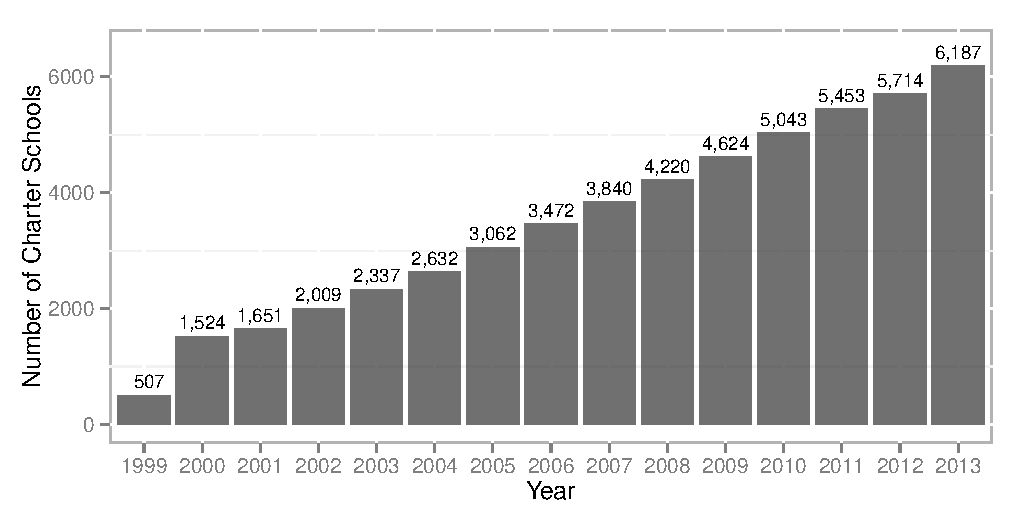
\includegraphics[width=\textwidth]{../Figures/CharterSchoolGrowth.pdf}
\caption{Charter School Growth 1999-2008}
\label{fig:charterSchoolGrowth}
\end{figure}

Clearly charter schools have become a popular vehicle for educational reform among parents as well. The \citeA{cersurvey} reports that 59\% of charter schools have waiting lists averaging 198 students. Charter schools provide an apparent choice to parents and are copacetic to the United State's individualistic \cite<see e.g.,>{hofstede2004,maccall1847,swart1962} culture. Moreover, like so many other fields, school reform has further emphasized marketization and privatization \cite{wells2002}. The influence of capitalism on education is not new. A major contributor to the expanded role of education during the industrial revolution is capitalism itself. That is, education expanded its initial purpose of providing a minimally informed electorate to providing an educated work force, not to mention keeping children off the streets as child labor laws came into existence. However, the shift of capitalistic principles from being the inspiration of educational reform to being the educational reform has profound implications.

Proponents of charter schools argue that public schools have been bogged down by bureaucracy and union contracts. Freeing schools of these requirements then allows teachers and schools to innovate, which in theory leads to increased student performance. The principled argument is the ``market metaphor" \cite{wells2002}. That is, if schools were forced to compete for ``customers" (i.e. students), then the differentiating factor between schools would be the quality of education. 

Opponents on the other hand have questioned the accountability, equity, effectiveness, and sustainability of charter schools. Several studies have shown that charter schools are not only failing to increase student performance, in many instances they are performing well under their traditional public school counterparts \cite<see e.g.,>{credo,braun06hlm,aft2004}. Others still argue whether charter schools may be a solution in search of a problem. \citeA{carnoy2005} in summarizing the controversy that ensued after the \citeA{aft2004} study argue that:

\begin{quote}
If, however, charter schools are not improving the achievement of disadvantages children, it may be that the cause of low student performance is not bureaucratic rules but something else. When a treatment is based on a diagnosis, and the treatment doesn't work, it is prudent to examine not only whether the treatment should be improved, but also whether the diagnosis might be flawed. \cite{carnoy2005}
\end{quote}

\subsection{Issues with Charter School Research}
The issues surrounding charter schools are immense. However, given the implications for the current and future generations of students, the issue must be explored using the best data and methods available. As \citeA{betts2006} point out, there are three major obstacles to addressing the question of ``whether students in charter schools are learning more or less than they would have learned in conventional schools" (p. 1), namely:

\begin{enumerate}
\item The issues of counterfactuals. That is, there are several barriers to determine the causal relationship between school choice and learning.
\item The variation in types of charter schools.
\item The nature of student achievement. Research has shown there are many other factors that contribute to student success including, but not limited to, social economic status, parents education, motivation, etc. The ability to decipher how school choice contributes to student learning in the context of all the other factors proves difficult.
\end{enumerate}

Though these issues are significant, they can to a large extent be reasonably addressed. We will not claim to fully account for these issues, however given the need for evidence to inform policy makers regarding charter school effectiveness, we will attempt to address these issues using the best data and methods available while clearly stating the limitations.

Issue one will be dealt with in more detail in chapter three. However, in short, the propensity score analysis (PSA) proposed for this study is arguably, assuming proper implementation, one of the best approaches to estimating causal inferences short of well designed randomized experiments. Of course in the context of an observational study the fundamental problem of causal inference \citeA{Holland1986} remains, but limitations of this will be addressed.

The issue of charter school variation is often cited in critiques of national or large scale charter school studies. Given that the charter school debate is a national debate that has implications at the Federal level, large scales studies are not only necessary, they are critical. If charter schools are to be offered wholly as an alternative to traditional public schools, then charter schools as a whole must be evaluated against public schools as a whole. More specifically, we wish not to evaluate whether a particular charter school, or type of charter school, is better, but whether the entire charter school concept is a better approach for educational reform.

Lastly, the environmental, social, community, and cultural factors that contribute to a student's academic achievement are often significantly underestimated. Often educational reform, as exemplified most recently by the No Child Left Behind Act, places the responsibility solely on the school without consideration of the context in which the school operates. We are encouraged by President Obama's remarks to his first Joint Session of Congress \cite{obama}:

\begin{quote}
These education policies will open the doors of opportunity for our children. But it is up to us to ensure they walk through them. In the end, there is no program or policy that can substitute for a mother or father who will attend those parent/teacher conferences, or help with homework after dinner, or turn off the TV, put away the video games, and read to their child. I speak to you not just as a President, but as a father when I say that \textit{responsibility for our children's education must begin at home} [emphasis added].
\end{quote}

\noindent Though we must be acutely aware and acknowledge the fact that schools are merely one factor of many that contribute to a students academic achievement, it does not preclude us from evaluating schools for their part. Similar to issue one, we argue that PSA provides an approach to best approximate the effects of school choice.

\subsection{Guiding Research Question}
Given that charter schools are being offered as a solution for the needed educational reform nationally, it is imperative that they be evaluated from a national perspective. This study proposes to compare the academic performance in two domains of charter schools and public schools using the National Assessment of Educational Progress and propensity score analysis. More specifically, this study proposes to address the question: Are there differences between charter and public schools? And if so, what is the nature and extent of those differences?



%==================== CHAPTER 2 ====================================================================
\cleardoublepage
\section{Chapter 2: Review of the Literature}

\subsection{History of Charter Schools}
Though Ray Budde is often credited with the current charter school movement \cite{kolderie05}, the term \textit{school choice} can be traced back to Adam Smith's \textit{Wealth of Nations}, Thomas Paine's \textit{Rights of Man}, and John Stuart Mill's \textit{On Liberty} \cite{herbst2006}. Prior to the Revolutionary War, given the religious diversity of colonial America, issues of education were left to local communities. However, after the war Revolutionary leaders argued that local schools were no longer sufficient for educating students for the emerging state and federal governments. It was Thomas Jefferson who, in 1779, introduced the first bill in Virginia that would establish a public school system. It was this, along with numerous other American intellects during the 1780s and 1790s, that established public schools throughout the young nation thereby relegating school choice to a choice between the public school and, predominately religious, private schools.

In the wake of the landmark report \textit{A Nation at Risk} \cite{nationatrisk}, \citeA{budde1988} authored a pivotal document that started the charter school movement in the United States. In this document, Budde argues that system-wide changes to the way schools are structured are required including: more rigorous curriculum and graduation standards; extended school days and year; more homework; teacher accountability for student results; termination of ``incompetent" teachers; and higher pay for teachers. To achieve these goals, he proposed a fundamental change to the ``internal organization of the school district... making substantial changes in the roles of teachers, principals, the superintedent, the school board, parents, and others in the community" (p. 16). More specifically, a framework for charter schools was proposed that includes five stages over a three year period (see Figure \ref{fig:timeline}). The five stages include: (1) generating ideas; (2) planning the charter; (3) preparing for teaching; (4) teaching under the educational charter; and (5) program monitoring and evaluation. For the first iteration of the cycle, stages one, two, and three occur prior to the opening of the school with stage one ideally beginning a full school year before. There are several features of this framework that deviate from traditional public school models, but most notably is the repetition of what may appear to be preparational stages. That is, the charter school must re-plan their school structure periodically (every three to five years according to Budde's framework) in a manner consistent to the initial charter school creation, thereby forcing a re-evaluation of the school bureaucracy.

\begin{figure}[tp]
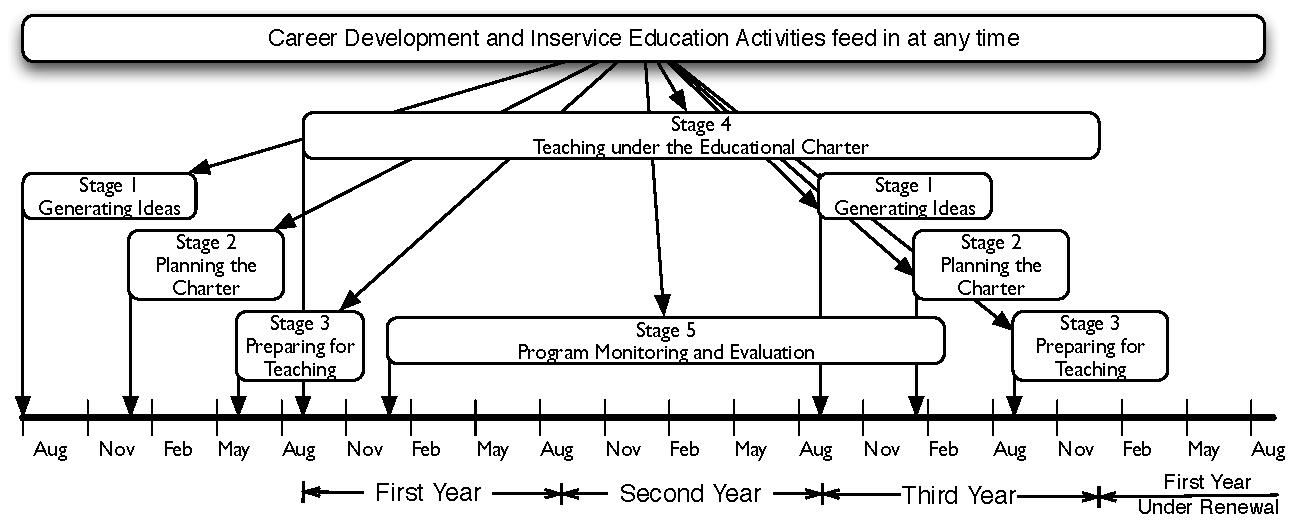
\includegraphics[width=\textwidth]{../Figures/Timeline.pdf}
\caption{Stages of a Charter School Life Cycle (adapted from Budde, 1988)}
\label{fig:timeline}
\end{figure}

Following the suggestions of Budde, Minnesota passed the first charter school law in 1991 with California being the second following in 1992. As of spring 2009, 40 states and the District of Columbia have charter school laws which comprise 1,407,421 students in 4,578 schools \cite{cernumbers}. According to \citeA{whatweknow}, there are currently over 200 studies that examine charter school achievement. 



\subsection{Empirical Evidence for Charter School Effectiveness}
Given that program evaluation and accountability are fundamental components of the philosophical foundations of charter schools, there are remarkably few \textit{high quality} empirical studies that address, at a national level, the academic effectiveness of charter schools \cite<c.f.>{whatweknow,betts2008}. That is not to say that there are not any studies that examine charter school achievement. The \citeA{whatweknow} provide a review of 140 studies selected on several criteria. Their review reveals significant gaps in the research with regard to states evaluated, research quality that addresses achievement, as well as timeliness of results. This is further exemplified by a meta-analysis conducted by \citeA{betts2008} that includes just 13 studies that represent nine states. In this section we will provide an overview of the current literature available vis-\`a-vis the published meta-analysis and literature reviews. We then focus on two recent studies that together provide the context for the study proposed here. More specifically, a hierarchical linear modeling analysis of the 2005 NAEP study \cite{braun06hlm} and a matching study comparing charter and public schools in 16 states \cite{credo}.

\subsubsection{Overview of Current Studies}
Research has shown that parents of students in charter schools are generally more satisfied with the charter school than the public school and will also tend to be more involved in their child's education \cite{teske2001,vanourek1998}. However, their satisfaction may simply be a rationalization \cite{hubbard2009}. Moreover, Fuller et al. \cite<1996, as cited in>{hubbard2009} suggest that parents that choose charter schools ``believe that the charter must therefore be superior to a conventional public school" (p. 177). This is collaborated by a study conducted by \citeA{cullen2005} that examines school choice in Chicago Public Schools whereby more than half of students elect to attend another Chicago Public School (e.g. career academy, high-achieving school) rather than their locally assigned school. Though students who opt out of their local school are more likely to graduate, \citeA{cullen2005} argue that ``those who opt out are superiour along unobservable dimensions such as their motivation level and parental involvement" (p. 755). 

The \citeA{whatweknow} provides perhaps the most comprehensive review of available research on charter school performance. The current report, \textit{Charter School Achievement: What We Know} is now in its fifth edition having been updated periodically to account for recent studies. In addition to covering published research reports, the review includes unpublished reports including conference presentations, dissertations, policy group and think tank reports, and state evaluations. Of the 210 studies identified, 140 are included in their review given that the study compares charter schools with traditional public schools, the study uses ``serious research methods" (p. 2), and ``examines a significant segment of the charter sector." The studies are then further categorized into one of three categories: (1) panel studies that are longitudinal and examine student growth over time; (2) cohort change studies that are longitudinal but use some other method than tracking individual students; and (3) snapshot studies that examine school performance at a single point in time (also known as observational studies).

Table \ref{charterAchievement} summarizes the findings of the 140 studies included first, by breaking out the year(s) the study's data is based upon, and second by the results reported. It should be noted that many of the pre-2001 studies were concentrated in a few states (Arizona, California, Florida, North Carolina, and Texas). This is expected given that these states are among the earliest to adopt charter school laws (see appendix A) as well as the substantial increase in the number of charter schools since 2000 (see figure \ref{fig:charterSchoolGrowth}). The National Alliance of Public Charter Schools conclude that:

\begin{quote}
[I]t becomes dramatically clear that studies examining public charter schools in more recent academic years show that charter schools produce more instances of larger achievement gains in both math and reading when compared to traditional public schools. (p. 3)
\end{quote}

\noindent However, this interpretation downplays the fact that approximately 30\% of charter schools performed worse than their traditional public school counterpart. These results are consistent with a recent by the \citeA{credo} that reported that 37\% of charter schools performed worse than their public school counterpart (this study is discussed in more detail below).



\begin{table}
\caption{Summary of studies on charter school achievement}
\label{charterAchievement}
\begin{center}
\begin{tabular}{lrrrrrrrrrr}
\thickline
            & \multicolumn{4}{c}{Pre 2001} & & \multicolumn{4}{c}{Post 2001}\\
            \cline{2-5} \cline{7-10}
            & Larger   & Similar   & Mixed    & Smaller    & & Larger    & Similar   & Mixed    & Smaller\\
            & Gains    & Gains     & Gains    & Gains      & & Gains     & Gains     & Gains    & Gains\\
\hline
Math        & 4      & 4      & 4      & 20     & & 17     & 17     & 1      & 14\\
            & (13\%) & (13\%) & (13\%) & (63\%) & & (35\%) & (35\%) &  (2\%) & (29\%)\\
Reading     & 7      & 10     & 3      & 14     & & 18     & 12     & 1      & 14\\
            & (21\%) & (29\%) &  (9\%) & (41\%) & & (40\%) & (27\%) &  (2\%) & (31\%)\\
\thickline
\multicolumn{10}{l}{Source: National Alliance of Public Charter Schools, 2009}\\
\end{tabular}
\end{center}
\end{table}

\citeA{betts2008} employ more stringent selection criteria for including studies in their meta-analysis. More specifically, only studies that used experimental student-level growth-based methods were included, resulting in a total of 14 studies published between 2001 and 2007 utilizing data ranging from 1998 through 2005. Similarly to \citeA{whatweknow}, studies included a limited number of locations including Arizona, California (three of which from San Diego specifically), Chicago, Delaware, Florida, Idaho, North Carolina, and Texas with one additional anonymous location. Overall, their analysis of the available studies provide very mixed results. However, some patterns to charter and public school differences emerge, specifically that charter schools generally outperform traditional public schools in elementary school reading and middle school math, though effect sizes for the latter are small. However, for high school reading and math charter schools are generally underperforming traditional public schools, but it should be noted that studies examining these grade levels is relatively small \cite<see also,>{whatweknow}.


\subsubsection{Two NAEP Studies Using HLM}
An increasingly used statistical method that allows for the analysis of studies where observations are not independent is hierarchical linear modeling (HLM), or multi-level analysis. In the context of the charter school question, comparing students in charter schools to public school counterparts with, say ordinary least squares or ANOVA, is inappropriate since these statistical models do not account for the school effects. HLM provides a model for which school effects can be partitioned from student effects thereby providing adjustments for the lack of independence of observations \cite<see e.g.,>{bryk1992,gelman2006}.

Braun, Jenkins, and Grigg have published two research reports utilizing NAEP and HLM that look at how public school students compare to private school students \citeyear{braun2006private} and charter schools students \citeyear{braun06hlm}. Note that the former study used the 2005 administering of NAEP whereas the latter used the 2003 administering of NAEP. A key advantage of using NAEP is that many student (see appendix C) and school level variables are available. Moreover, as of 2003 charter schools have been oversampled to ensure sufficient sample sizes for appropriate comparisons to be made. 

\paragraph{Comparing Private and Public Schools}
For the private school study \cite{braun2006private}, results found that students in private schools scored significantly higher than public school students in both mathematics and reading at grades 4 and 8. Differences ranged from 8 points for grade 4 mathematics to 18 points for grade 8 reading. Adjusting for student characteristics with HLM resulted in reductions in all four comparisons of approximately 11 to 14 points. After adjustment, private school students still scored significantly higher than public school students in grade 8 reading, but public schools scored significantly better in grade 4 mathematics. There was no significant difference for grade 4 reading and grade 8 mathematics.

\paragraph{Comparing Charter and Private Schools}
For the charter school study \cite{braun06hlm} analysis was conducted in three phases for both reading and mathematics. In phase one, all charter schools were compared to all public schools. Results found that, when student characteristics were adjusted for, charter schools performed on average 4.2 points lower than publics schools in reading (corresponding effect size is 0.11 standard deviations) and 4.7 points lower in mathematics (corresponding effect size is 0.17 standard deviations). 

Phase two separated charter schools into two groups: charter schools that are associated with a public school district (PSD) and those that are not. Separate analysis were performed for each charter school type with public schools. For reading, there was no significant difference between charter schools affiliated with a PSD and public schools. However, for schools not affiliated with a PSD, charter school students scored significantly lower than public school students with an adjusted difference of 0.17 standard deviations. Similarly for mathematics, there was no difference between charter schools affiliated with a PSD and public schools but charter schools not affiliated with PSD scored significantly lower with an adjusted difference of 0.23 standard deviations.

Lastly, phase three compared only charter and publics schools located in a central city and serving a high-minority population. For reading, there was no significant difference between charter and public schools for any model. For mathematics however, charter schools not affiliated with a PSD scored significantly lower than public school students with an adjusted difference of 0.17 standard differences. There was no difference for schools affiliated with a PSD.


\subsubsection{The CREDO Study}
The \citeA{credo} conducted a study of more than 1.7 million records from 2400 charter within 16 states. The methodology involves creating a Virtual Control Record (VCR) for each charter school student \cite<see also,>{abadie2007,nea} which is used to find matching student from an eligible traditional public school. Students within a traditional public school become available in a pool of potential matches when at least one student is identified as transferring to a charter school. Once the ``feeder schools" are identified, all students from feeder schools are pooled and serve as the source to select matches to the charter school students. Students are then matched on the following factors: grade-level, gender\footnote{Gender was not available in Florida}, race/ethnicity, free or reduced price lunch status, English language learner status, special education status, and prior test score on state achievement tests. This procedure, which is similar to propensity matching, resulted in 83.7\% and 84.4\% of charter school students being matched to a public school student for reading and math, respectively.

Once matches were determined, ordinary least squares regression was utilized to analyze both math and reading scores, separately, across the charter school students and matched public school students. Moreover, controls for student characteristics used above, excluding gender, along with state indicators and scores affected by Hurricane Katrina, were added to the basic model. Overall results show that charter school students performed, on average, 0.01 and 0.03 standard deviations below public school students for reading and math, respectively. Both results are significant at \textit{p} $\leq$ 0.01.

Though the magnitude of the overall effects may not necessarily suggest charter schools are performing substantially lower than their public school counterparts, further analysis by \citeA{credo} reveal more nuanced understanding of the differences. More specifically, the effectiveness of charter schools varied considerably by state. Five states (Arkansas, Colorado, Illinois, Louisiana, \& Missouri) were found to have higher learning gains for charter schools. Six states (Arizona, Florida, Minnesota, New Mexico, Ohio, \& Texas) were found to have lower learning gains for charter schools. The remaining four states (California, District of Columbia, Georgia, \& North Carolina) had either mixed results or no difference in academic gains. 

Lastly, the \citeA{credo} found variation of charter school effectiveness across school characteristics. That is, schools that focused on elementary or middle grades separately, tended to perform as well or better than their public school counterparts. However, for charter schools that focused on high grades or multi-level grades performed anywhere from .02 to .08 standard deviations below public schools. Moreover, school level comparisons find that only 17\% of charter schools perform better than public schools while 46\% perform no differently and 37\% perform significantly worse.

%\paragraph{Criticisms of the CREDO Study}




%==================== CHAPTER 3 ====================================================================
\cleardoublepage
\section{Chapter 3: Method}
This chapter will outline the methods that will be utilized to describe and analyze the data in order to address the research questions central to this study. Given the strong political interests in the question of charter school effectiveness and the implications for educational policy both at the state and national level, obtaining good empirical evidence, preferably with strong causal inferences, is most desirable. The \textit{gold standard} of inferential research is the randomized experiment. A research design that addresses the charter school question proposed here would require that students be randomly assigned, possibly with blocking on key covariates, to either a charter or public school. The theoretical justification for such a scheme is that any systematic differences between the two groups would be balanced through the randomization processes. However, in practice, especially in education, such randomization is neither feasible nor ethical. The result of the lack of randomization is a phenomenon called selection bias. That is, any comparisons of the two groups will be biased given the fact that the units of study, students in this study, self-selected to be in their respected group. Propensity score analysis \cite{rosenbaum83} is a statistical approach whereby the differences between the two groups are balanced by the careful analysis of covariate information. This procedure lends itself well to secondary analysis of observational data.

\subsection{Overview of NAEP}
The source of the data that will be utilized in this study is provided by the National Center for Educational Statistics (NCES) which is within the U.S. Department of Education's Institute of Education Sciences (IES). The National Assessment of Educational Progress (NAEP) was started in 1971 and has provided national measures of student achievement in many subjects including mathematics, reading, science, writing, history, civics, and the arts. In 2003 NAEP began assessing charter schools as well as private and public schools. This study will utilize the 2007 administering of the NAEP assessments in mathematics and reading within grades four and eight. The 2007 assessment included over 6,000 public schools and over 200 charter schools comprising of over 145,000 and 3,000 students, respectively. Given this relatively large, nationally representative sample, analysis of NAEP assessments utilizing propensity score analysis may prove to provide valuable insights into the academic differences between charter and public schools.

More than simply providing large samples, another key advantage of NAEP is the fact that it is not designed to assess individual students or schools, but instead is designed to inform subject-matter achievement, instructional experiences, and school environments (Braun, Jenkins, \& Grigg, 2006). To achieve this goal, NAEP utilizes a complex item-sampling design such that individual students are presented a subset of the total items, thereby reducing the burden on participants. Though not appropriate for assessing individual student achievement, in aggregate the NAEP measures provide a robust and accurate estimate of student achievement.

In addition to subject area measures, NAEP includes student, teacher, and school questionnaires that provide contextual information about the students' environment. Given that PSA relies on adjusting for selection bias by adjusting for known covariates, it are the answers to these questionnaires that will serve as the basis for determining a students propensity score, or likelihood of being in the treatment (i.e. charter school in the context of this study). In addition to typical demographic items such as gender and race, students are asked about computers, books, magazines, and encyclopedias in the home; parents education level; and the level of interaction with academics within the home (see appendix C for complete list of items).

The responsibility for developing the assessment objectives and test specifications lies with the National Assessment Governing Board which was created by Congress in 1988. Traditionally they are the states that have provided the legal guidance for school governance including accountability measures. Given the varied standards across states, it is this governing board that is to determine nationally what are appropriate achievement goals for each age and grade. The following two sections will provide the framework for mathematics and reading assessments.

\subsubsection{Mathematics}
Since 1990, the Council of Chief State School Officers (CCSSO) has been contracted to design a framework for the mathematics assessment \cite{naepmath}. The framework was most recently updated in 2000 to take into account state standards, the National Council of Teachers of Mathematics (NCTM) standards, the Trends International Mathematics and Science Study (TIMSS), the Achieve Project, and a 2001 report issued by the National research Council of the National Academy of Sciences. The result of their work was six recommendations for the mathematics assessment regarding content areas, mathematical complexity of items, distribution of items, item formats, manipulatives, and calculators. For the purposes of the study proposed, a composite score will be utilized that is comprised of five content areas, number properties and operations; measurement; geometry; data analysis and probability; and algebra. Table \ref{naepMathContent} provides details regarding the distribution of items comprising the composite score for the grade four and eight assessments.

\begin{table}
\caption{Distribution of Math Items by Grade and Content Area}
\label{naepMathContent}
\begin{center}
\begin{tabular}{lrr}
\thickline
Content Area                     & Grade 4 & Grade 8\\ \hline
Number Properties and Operations & 40\%    & 20\% \\
Measurement                      & 20\%    & 15\% \\
Geometry                         & 15\%    & 20\% \\
Data Analysis and Probability    & 10\%    & 15\% \\
Algebra                          & 15\%    & 30\% \\
\thickline
\end{tabular}
\end{center}
\end{table}


\subsubsection{Reading}
The NAEP Reading Framework (2006) provides guidelines and a theoretical basis for reading assessment. This framework is designed with the input of individuals and organizations involved in reading education including researchers, policymakers, teachers, and business representatives. However, a particular emphasis is placed on the work of the National Institute for Child Health and Human Development (NICHID). More specifically, the NICHID summarizes how the research describes a reader as:

\begin{quote}
In the cognitive research, reading is purposeful and active. According to this view, a reader reads a text to understand what is read, to construct memory representations of what is understood, and to put this understanding to use. \cite<p. 4, NICHD, 2000, as cited in>{naepreading}
\end{quote}

\noindent Moreover, reading is considered to be a complex process rather than a simple set of skills. As such, the NAEP reading assessment is designed such that comprehension is defined as:

\begin{quote}
``[I]ntentional thinking during which meaning is constructed through interactions between text and reader" (Harris \& Hodges, 1995). Thus, readers derive meaning from text when they engage in intentional, problem solving thinking processes. \cite<p. 14, NICHD, 2000, as cited in>{naepreading}
\end{quote}

\noindent Given this framework, NAEP provides an excellent tool for evaluating overall reading achievement, but not to diagnosis specific individuals.

The NAEP reading assessment is designed to account for three reading contexts: reading for literacy experience, reading for information, and reading to perform a task. Within these contexts, four aspects of reading are considered: forming a general understanding, developing interpretation, making reader/text connections, and examining content and structure. The reading assessment is administered by supplying students with booklets that contain reading materials and comprehension questions. The questions consist of both multiple-choice and constructed-response question formats with at least half of the questions being of the constructed-response type. 


\subsection{Analysis}



\subsubsection{Phase I}
Propensity score analysis \cite<PSA;>{rosenbaum83} is a statistical method or approach that attempts to adjust for selection bias in observational studies and has become increasingly popular in medical research \cite{Austin2008} and in the social sciences \cite{ThoemmesKim2011}. 

Most of the studies conducted using PSA involve analysis in two phases where phase one involves the the calculation of propensity scores or matching for both treatment and control units of analysis; and phase two involves the comparison of those two groups. However, in situations where data is multilevel, or clustered, special consideration is necessary both at phase I and II. For the NAEP data, the state variable will be used as the level 2 identifier. The algorithm in the \texttt{multilevelPSA} package \citeA{Bryer2011} will facilitate the multilevel PSA analysis. Specifically, for phase I, three approaches will be used for stratifying students for comparison, namely conditional inference trees \citeA{HorthornHornikZeileis2010}, logistic regression, and matching. For each approach, the stratification procedure will be performed separately for each state so that direct comparisons between students in phase II do not occur between states. That is, students within a stratification or two students being matched must reside in the same state.

\subsubsection{Phase II}
The second phase of the propensity score analysis involves comparing dependent variables of students with similar propensity scores using standard \textit{t}-tests and reporting corresponding confidence intervals and effect sizes. However, for multilevel data analysis occurs in two states. First, comparisons are made for each state. The results from each state can then be aggregated to provide an overall difference and effect size. 

\subsubsection{Graphical Representation}
Given the large amount of data that needs to be summarized, the use of graphics will be emphasized. The \texttt{multilevelPSA} package provides a number of graphing functions that extend the framework introduced by Helmreich and Pruzek for multilevel PSA. Figure \ref{fig:g8math:circ} represents a multilevel PSA assessment plot. In this graphic, the x-axis corresponds public school grade 8 NAEP scores and the y-axis corresponds to charter school grade 8 NAEP scores. Each colored circle is a state with its size corresponding the number of students within each state. The distribution of differences between charter and public schools across states are represented as tick marks along the diagonal line in the bottom left of the graphic. Differences are aggregated (and weighted by size) across states. For grade 8 math, the overall adjusted mean for charter school students is 281 and the overall adjusted mean for public school student is 278. The dashed blue line parallel to the unit line corresponds to the overall adjusted mean difference and likewise, the dashed green lines correspond to the confidence interval.

\begin{figure}[tp]
\begin{center}
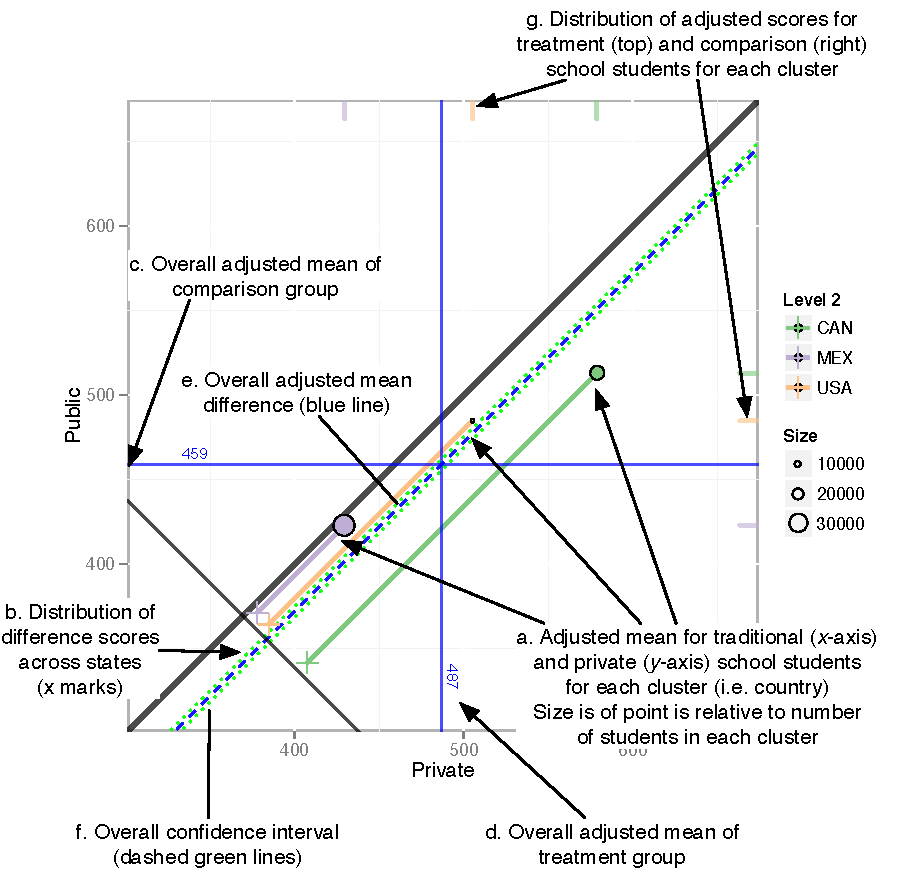
\includegraphics[width=\textwidth]{../Figures/AnnotatedCircPlot.pdf}
\caption{Multilevel PSA Assessment Plot: Grade 4 Math}
\label{fig:g8math:circ}
\end{center}
\end{figure}


Figure \ref{fig:g8math:diff} provides a more nuanced depiction of the differences both between and across states. Similar to the mutlielvel PSA assessment plot, each blue dot corresponds to a state and is sized relative to the number of students within each state. The light gray dots correspond to each of the strata within each state. The graphic also provides confidence intervals for each state as well as the overall adjusted mean difference and confidence interval.

\begin{figure}[tp]
\begin{center}
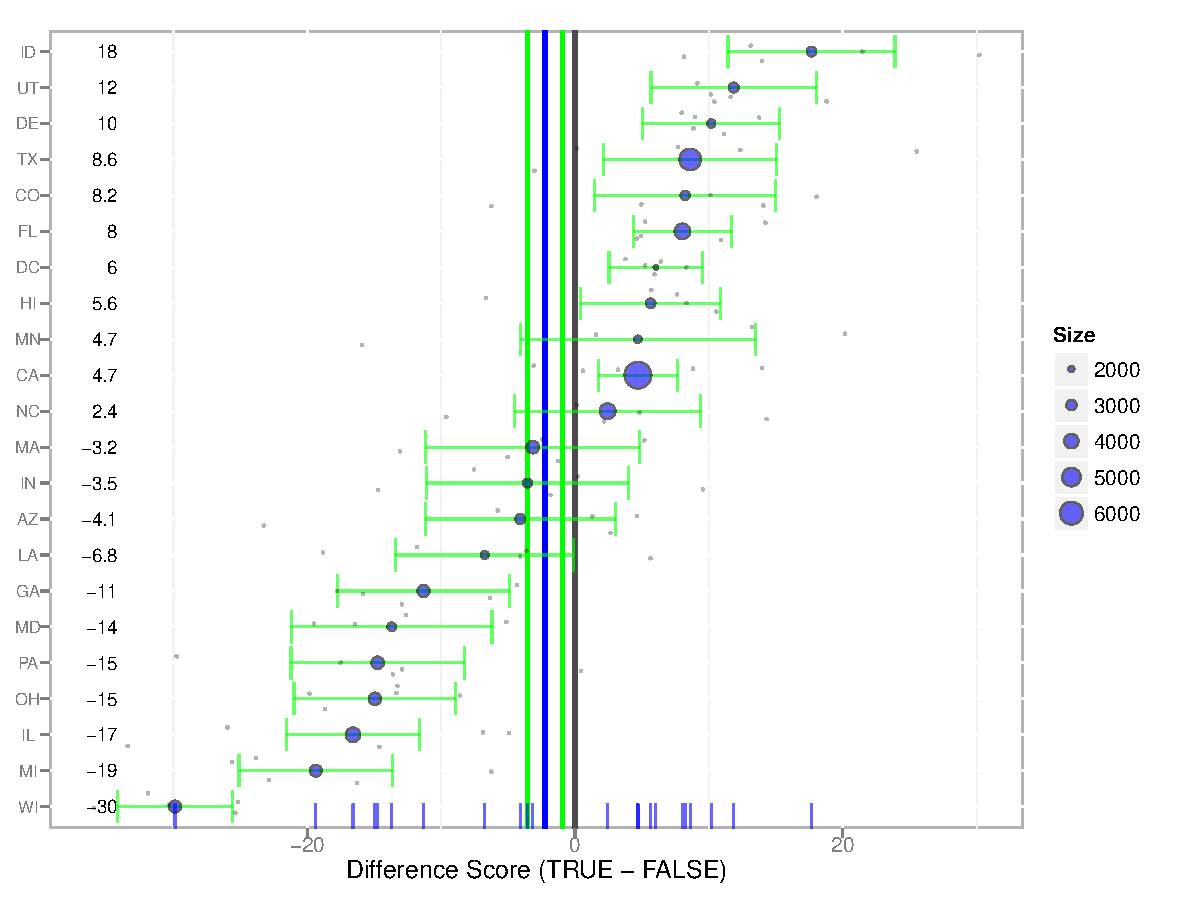
\includegraphics[height=\textwidth]{../Figures2009/g8math-mlpsa-lr-diff.pdf}
\caption{Multilevel PSA Difference Plot: Grade 8 Math}
\label{fig:g8math:diff}
\end{center}
\end{figure}


%==================== CHAPTER 4 ====================================================================
\cleardoublepage
\section{Chapter 4: Results}

In this chapter I will outline in detail the results of all the propensity score models described in chapter three. Since NAEP is organized such that each grade and subject combination is a separate dataset, this chapter will focus on the analysis of grade four math. The results for grade four reading, grade eight math, and grade eight reading are included in the appendices. The chapter begins with a discussion of data preparation, followed by details of the nine propensity score methods used, and concludes with a summary, including tables and figures, of the overall results across all grades and subjects.

All analysis was conducted using R \cite{redevelopment}\footnote{All R scripts are available from Github at \url{https://github.com/jbryer/Dissertation}. Due to the licensing agreement with NCES, data is not included. However, researchers with access to the 2009 restricted use data should be able to replicate the analysis outlined in this chapter.}. R provides a number of advantages over other applications including a framework for extending its core functionality through R packages. I have written and published two R packages primarily for conducting the analysis in this dissertation. The \texttt{naep} package provides functions to read and work with the National Assessment of Educational Progress (NAEP) data sets. Secondly, the \texttt{multilevelPSA} package provides functions to conduct multilevel propensity score analysis as described above. Both of these packages are available from the Comprehensive R Archive Network (CRAN). 

\textit{Formatting note}. Since the development of the R packages are in and of themselves a major component of this dissertation, I will make reference to some of the functions available. All references to R packages and functions will appear in a \texttt{fixed width font}.

\subsection{Data Preparation}


\subsubsection{Missing Data Imputation}
Stratification by logistic regression (using two approaches to covariate selection) and matching require a complete dataset to estimate the models. As such, missing data was imputed using multivariate imputation by chained equations \citeA{vanbuuren} vis-\`a-vis the MICE package \citeA{mice} in R.


% latex table generated in R 3.0.1 by xtable 1.7-1 package
% Tue Jun 11 07:43:51 2013
\begin{table}[ht]
\centering
\caption{Descriptive Statistics of Dependent Variables (Unadjusted)} 
\label{dependentDescriptives}
\begin{tabular}{lrr@{\extracolsep{.2cm}}rrrrr}
  \hline
   & \multicolumn{2}{c}{Charter} & \multicolumn{2}{c}{Public} & Mean & \multicolumn{2}{c}{Confidence} \\ \cline{2-3} \cline{4-5}  Subject & Mean & SD & Mean & SD & Difference & \multicolumn{2}{c}{Interval} \\  \hline
Grade 4 Math & 231.2 & 28.3 & 237.3 & 28.5 & -6.0 & -7.0 & -5.0 \\ 
  Grade 4 Reading & 212.9 & 33.0 & 217.1 & 34.5 & -4.2 & -5.3 & -3.1 \\ 
  Grade 8 Math & 271.8 & 35.5 & 279.4 & 35.8 & -7.5 & -8.7 & -6.4 \\ 
  Grade 8 Reading & 256.2 & 32.9 & 259.8 & 32.6 & -3.6 & -4.7 & -2.6 \\ 
   \hline
\end{tabular}
\end{table}


\begin{figure}[ht]
\begin{center}
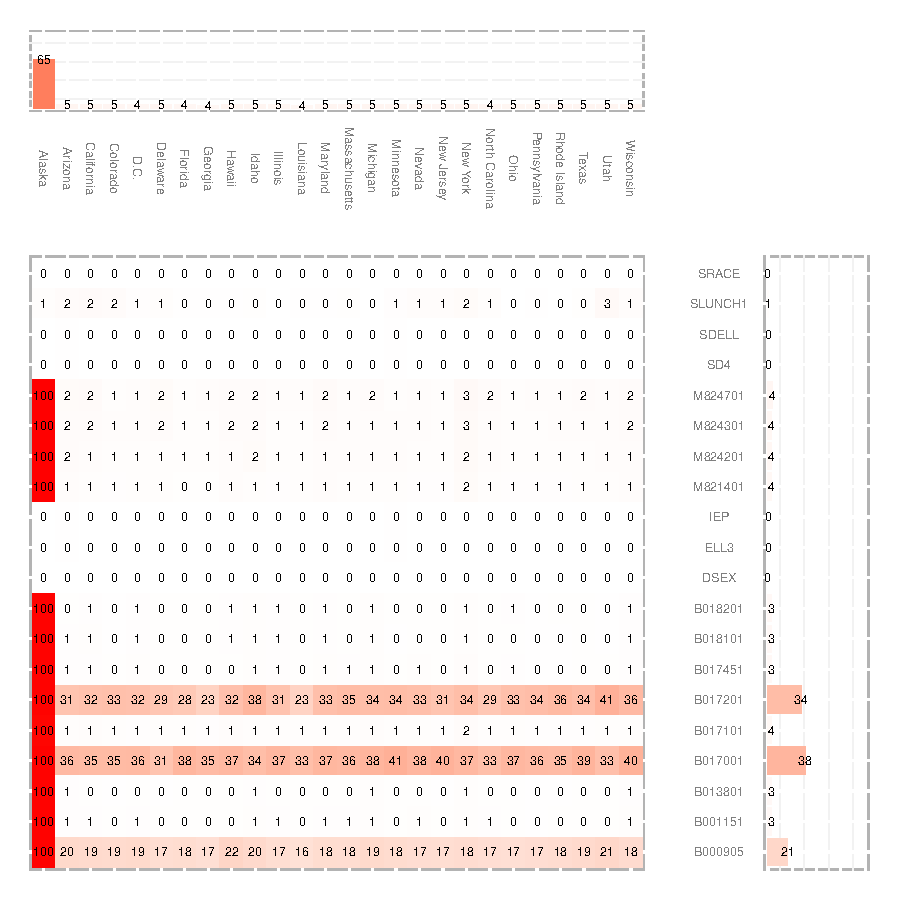
\includegraphics[width=\textwidth]{../Figures2009/g4math-missing.pdf}
\caption{Missing Data Plot: Grade 4 Math}
\label{fig:g4math:missing}
\end{center}
\end{figure}



\subsection{Propensity Score Analysis

\subsubsection{Propensity Score Analysis with Stratification}


\begin{figure}[ht]
\begin{center}
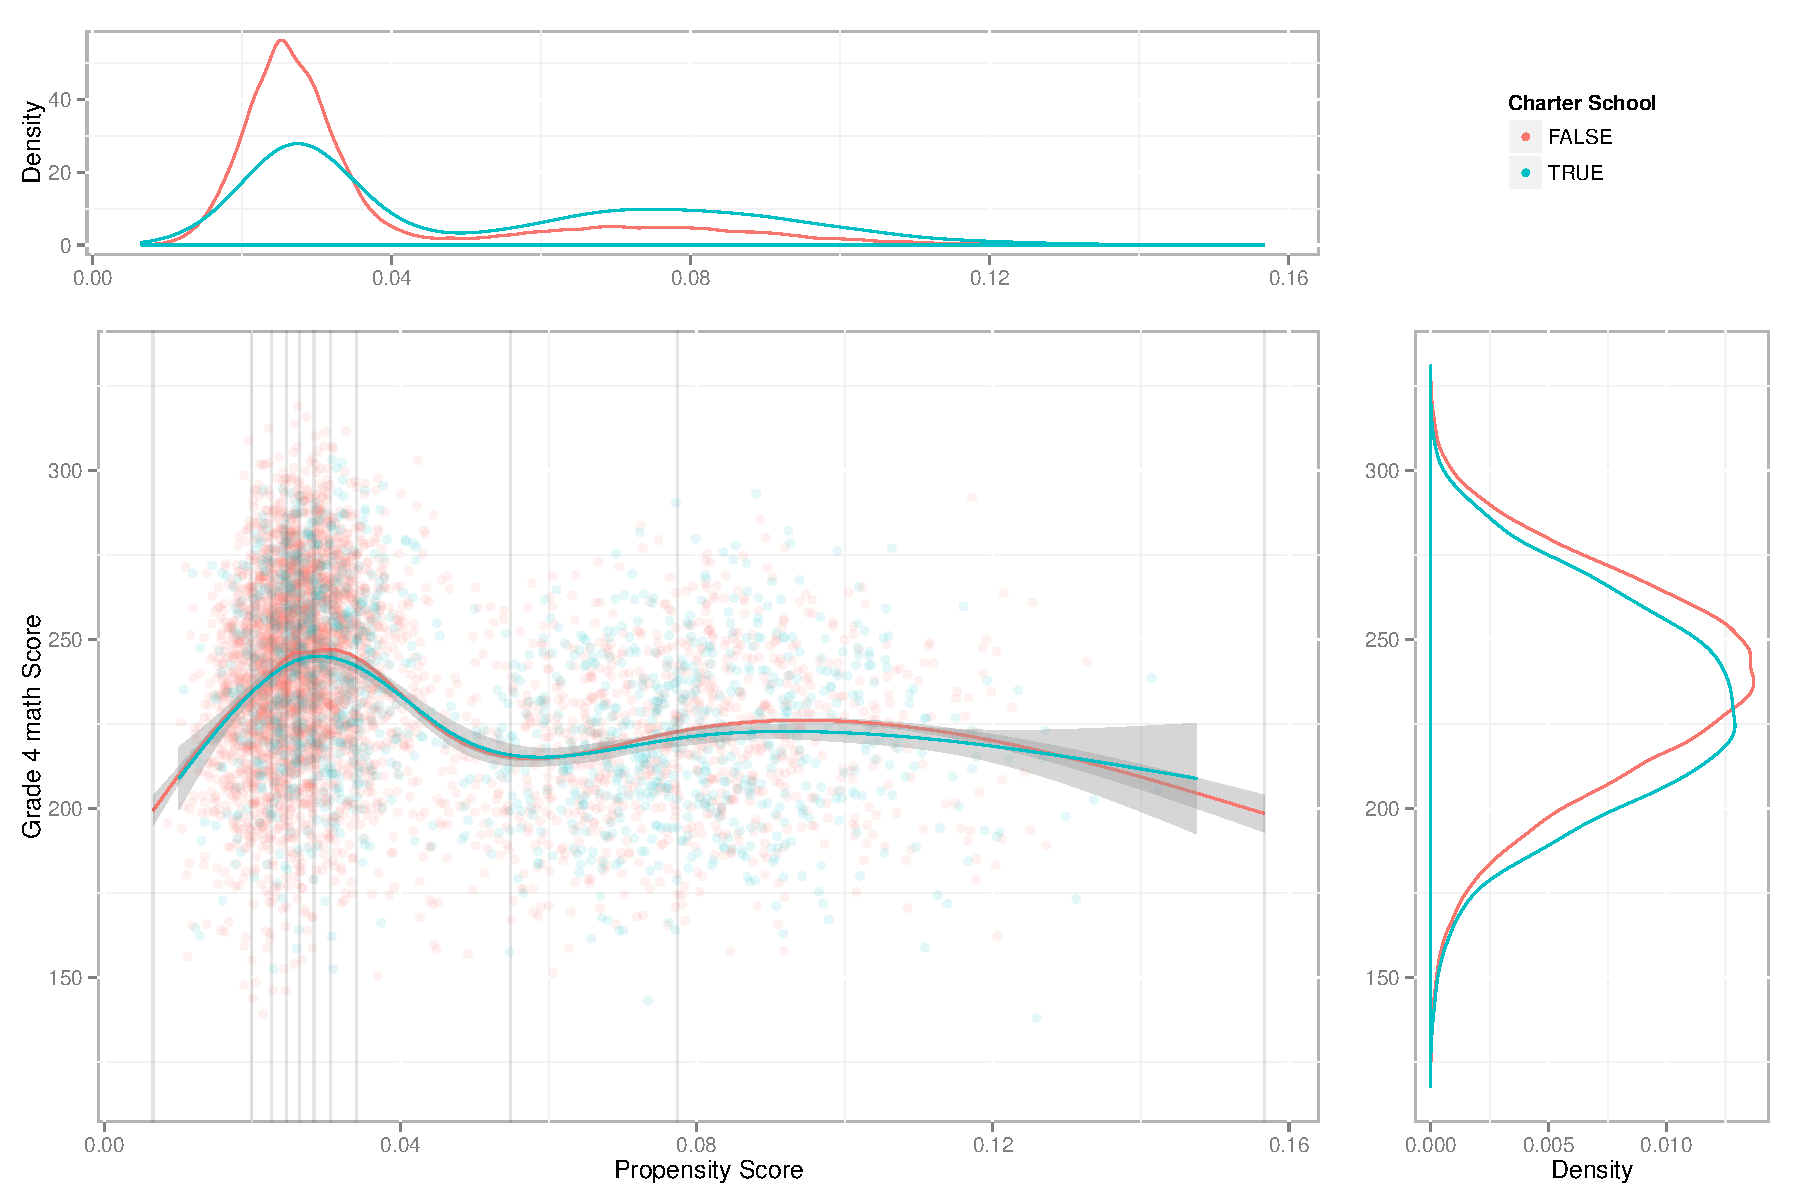
\includegraphics[width=\textwidth]{../Figures2009/g4math-loess.pdf}
\caption{Loess Regression Assessment Plot: Grade 4 Math}
\label{fig:g4math:loess}
\end{center}
\end{figure}

\begin{figure}[ht]
\begin{center}
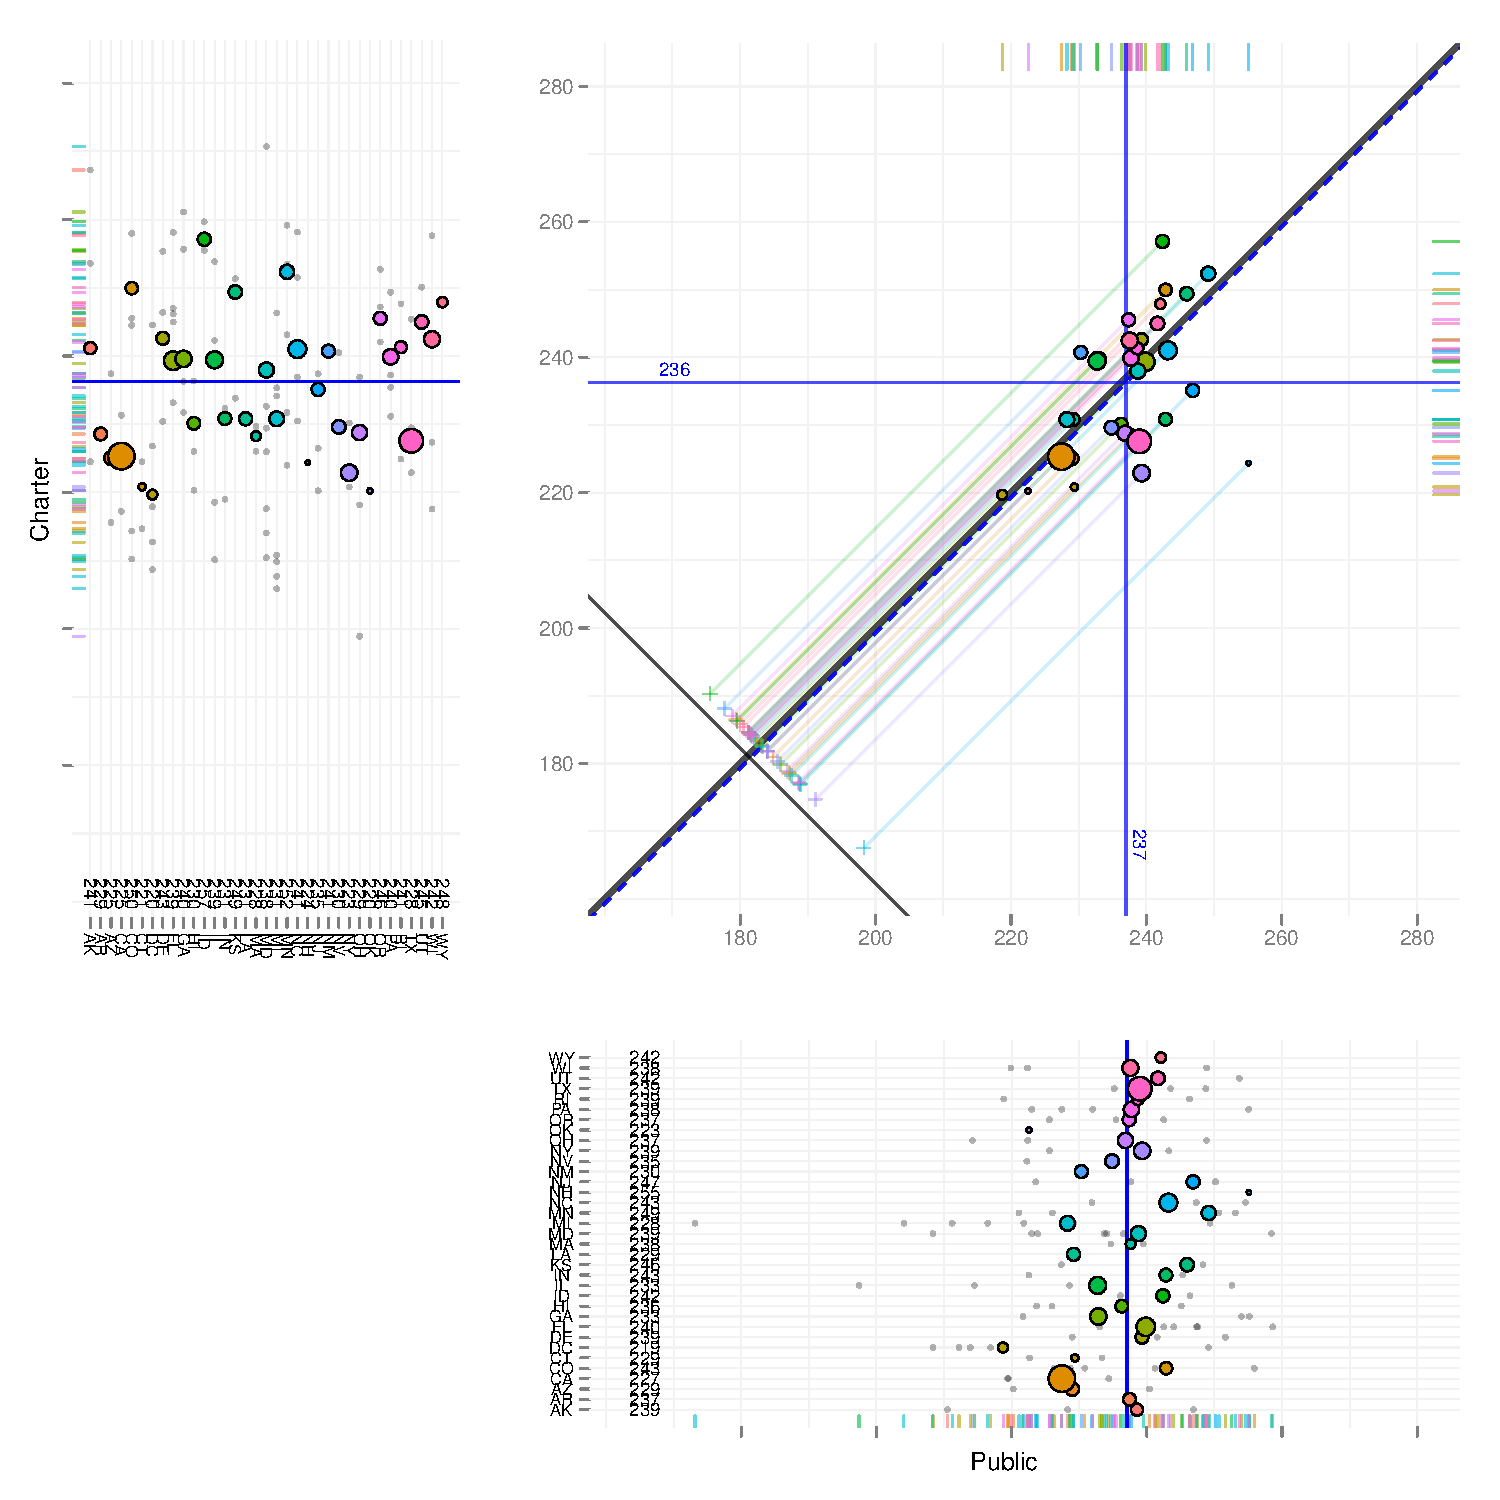
\includegraphics[width=\textwidth]{../Figures2009/g4math-mlpsa-ctree.pdf}
\caption{Multilevel PSA Assessment Plot: Grade 4 Math}
\label{fig:g4math-mlpsa-ctree}
\end{center}
\end{figure}

\begin{figure}[ht]
\begin{center}
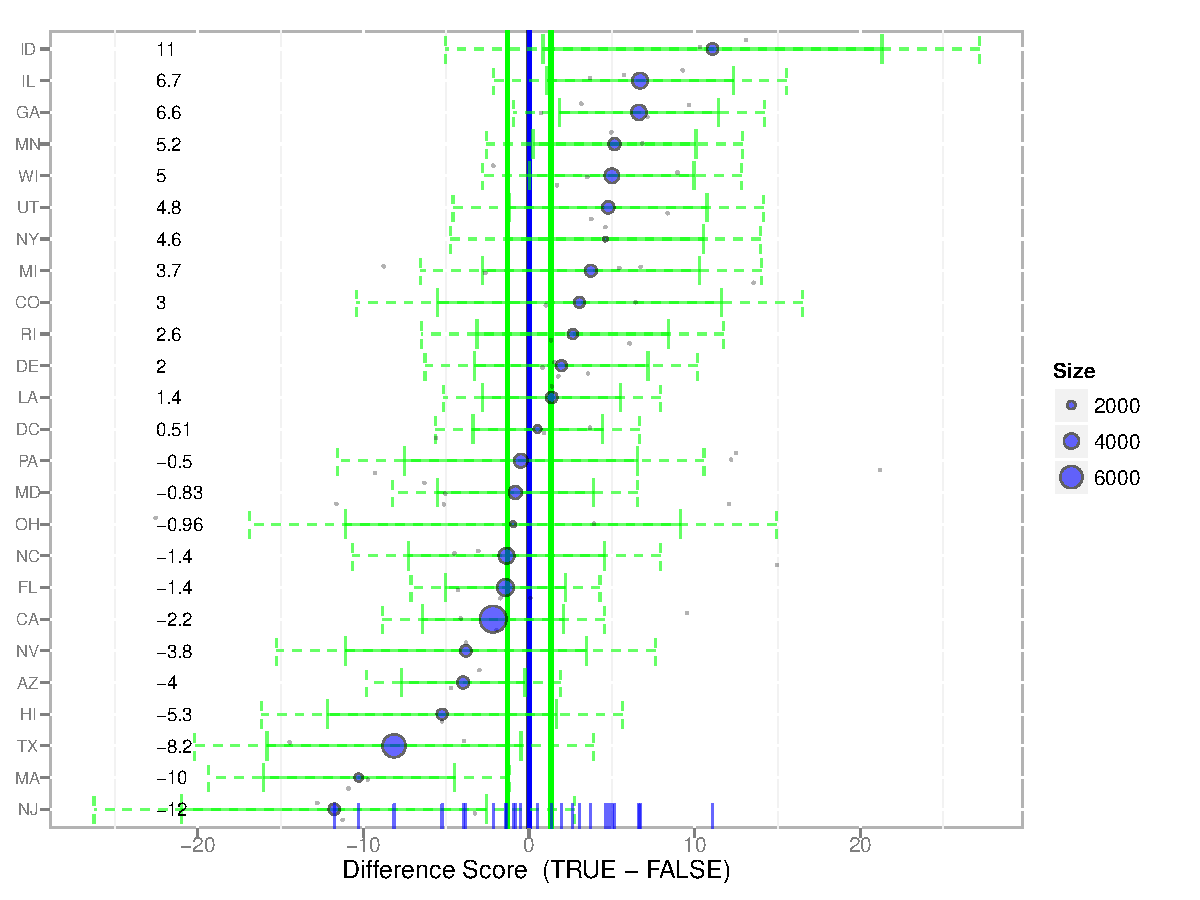
\includegraphics[width=\textwidth]{../Figures2009/g4math-mlpsa-ctree-diff.pdf}
\caption{Multilevel PSA Difference Plot: Grade 4 Math}
\label{fig:g4math-mlpsa-ctree-diff}
\end{center}
\end{figure}


%\begin{singlespace}
%% latex table generated in R 2.14.1 by xtable 1.6-0 package
% Wed Mar 14 20:50:46 2012
\begin{longtable}{lcrr@{\extracolsep{10pt}}rr@{\extracolsep{10pt}}r}
\caption{Level 1 Summary Grade 4 Math (CITs)} \\ 
   \thickline State & Strata & \multicolumn{2}{c}{Public} & \multicolumn{2}{c}{Charter} & Diff \\ \cline{3-4} \cline{5-6} & & Mean & n & Mean & n & \\ \hline\endfirsthead \multicolumn{7}{l}{...continued from previous page} \\ \thickline State & Strata & \multicolumn{2}{c}{Public} & \multicolumn{2}{c}{Charter} & Diff \\ \cline{3-4} \cline{5-6} & & Mean & n & Mean & n & \\ \hline \endhead \thickline \multicolumn{7}{r}{continued on next page...} \\ \endfoot \multicolumn{7}{c}{} \\ \endlastfoot AK & 2 & 228.3 & 1096 & 224.5 & 25 & -3.8 \\ 
  AK & 4 & 210.5 & 16 & 267.3 &  7 & 56.8 \\ 
  AK & 5 & 246.9 & 1384 & 253.6 & 70 & 6.7 \\ 
  AR & 1 & 237.4 & 2776 & 228.6 & 16 & -8.9 \\ 
  AZ & 2 & 240.4 & 1185 & 237.4 & 143 & -3.0 \\ 
  AZ & 3 & 220.2 & 1651 & 215.6 & 83 & -4.7 \\ 
  CA & 3 & 219.5 & 2802 & 217.2 & 79 & -2.3 \\ 
  CA & 4 & 234.4 & 3850 & 231.3 & 55 & -3.1 \\ 
  CA & 9 & 219.4 & 498 & 225.0 & 35 & 5.6 \\ 
  CO & 10 & 182.0 & 10 & 148.2 &  1 & -33.9 \\ 
  CO & 11 & 228.7 & 954 & 245.5 & 13 & 16.8 \\ 
  CO & 4 & 230.8 &  7 & 210.2 &  3 & -20.6 \\ 
  CO & 5 & 241.2 & 378 & 244.5 & 30 & 3.3 \\ 
  CO & 6 & 255.9 & 1127 & 258.0 & 81 & 2.1 \\ 
  CO & 9 & 226.3 & 74 & 214.3 &  4 & -11.9 \\ 
  CT & 3 & 233.4 & 572 & 224.5 &  7 & -8.9 \\ 
  CT & 5 & 222.7 & 327 & 214.7 & 19 & -8.0 \\ 
  DC & 3 & 216.9 & 31 & 226.8 & 12 & 9.9 \\ 
  DC & 4 & 249.1 & 263 & 244.6 & 36 & -4.6 \\ 
  DC & 7 & 212.2 & 546 & 212.7 & 208 & 0.5 \\ 
  DC & 8 & 208.4 & 112 & 208.7 & 22 & 0.3 \\ 
  DC & 9 & 213.9 & 330 & 217.9 & 234 & 4.0 \\ 
  DE & 2 & 229.0 & 929 & 230.4 & 107 & 1.4 \\ 
  DE & 4 & 251.6 & 615 & 255.3 & 56 & 3.7 \\ 
  DE & 5 & 241.5 & 1042 & 246.4 & 32 & 4.9 \\ 
  FL & 10 & 258.6 & 680 & 258.1 & 29 & -0.5 \\ 
  FL & 11 & 244.0 & 377 & 238.9 & 38 & -5.0 \\ 
  FL & 2 & 233.0 & 2780 & 233.1 & 69 & 0.1 \\ 
  FL & 4 & 247.4 & 483 & 245.0 & 16 & -2.4 \\ 
  FL & 6 & 242.5 & 191 & 246.2 & 11 & 3.7 \\ 
  FL & 9 & 247.5 & 20 & 247.0 &  3 & -0.5 \\ 
  GA & 2 & 221.7 & 2354 & 231.7 & 77 & 10.0 \\ 
  GA & 4 & 254.0 & 152 & 261.1 &  5 & 7.1 \\ 
  GA & 6 & 233.3 & 358 & 236.3 & 23 & 3.0 \\ 
  GA & 7 & 255.2 & 1001 & 255.7 & 59 & 0.5 \\ 
  HI & 2 & 245.1 & 1558 & 236.3 & 35 & -8.8 \\ 
  HI & 4 & 226.0 & 255 & 226.0 &  8 & 0.1 \\ 
  HI & 5 & 223.7 & 882 & 220.3 & 14 & -3.4 \\ 
  ID & 2 & 246.4 & 1746 & 255.5 & 52 & 9.1 \\ 
  ID & 4 & 212.7 & 139 & 231.0 &  2 & 18.3 \\ 
  ID & 5 & 236.1 & 1139 & 259.7 &  6 & 23.6 \\ 
  IL & 2 & 197.4 & 97 & 210.1 &  6 & 12.7 \\ 
  IL & 4 & 214.5 & 1041 & 218.6 & 37 & 4.1 \\ 
  IL & 6 & 252.6 & 1475 & 253.8 &  8 & 1.3 \\ 
  IL & 7 & 228.5 & 1446 & 242.3 & 27 & 13.7 \\ 
  IN & 2 & 222.6 & 296 & 219.0 &  8 & -3.6 \\ 
  IN & 3 & 245.3 & 2466 & 232.3 &  5 & -13.0 \\ 
  KS & 2 & 227.3 & 324 & 233.8 &  7 & 6.5 \\ 
  KS & 3 & 248.3 & 2616 & 251.3 & 21 & 3.0 \\ 
  LA & 1 & 229.2 & 2830 & 230.8 & 65 & 1.6 \\ 
  MA & 2 & 239.5 & 986 & 229.7 & 37 & -9.8 \\ 
  MA & 4 & 234.7 & 654 & 226.0 & 12 & -8.6 \\ 
  MA & 6 & 257.5 & 1952 & 234.0 &  2 & -23.5 \\ 
  MD & 11 & 234.1 & 364 & 226.0 &  8 & -8.1 \\ 
  MD & 12 & 236.5 & 168 & 232.6 & 10 & -3.9 \\ 
  MD & 13 & 258.5 & 1209 & 270.7 & 10 & 12.3 \\ 
  MD & 4 & 223.0 & 324 & 217.6 & 22 & -5.3 \\ 
  MD & 5 & 233.7 & 379 & 229.4 &  6 & -4.3 \\ 
  MD & 7 & 223.9 & 728 & 210.4 & 84 & -13.4 \\ 
  MD & 8 & 208.4 & 77 & 214.0 &  1 & 5.7 \\ 
  MI & 11 & 173.2 &  3 & 205.9 &  3 & 32.7 \\ 
  MI & 12 & 229.2 & 652 & 235.3 & 19 & 6.2 \\ 
  MI & 13 & 216.5 &  9 & 207.7 &  5 & -8.8 \\ 
  MI & 2 & 204.1 & 981 & 210.8 & 144 & 6.7 \\ 
  MI & 4 & 249.3 & 1384 & 246.3 & 18 & -3.0 \\ 
  MI & 7 & 211.2 & 97 & 209.9 &  5 & -1.4 \\ 
  MI & 8 & 221.8 & 78 & 234.2 & 21 & 12.4 \\ 
  MN & 10 & 250.7 & 2150 & 253.5 & 39 & 2.8 \\ 
  MN & 11 & 253.1 & 594 & 259.2 & 33 & 6.1 \\ 
  MN & 3 & 248.4 & 172 & 243.1 &  3 & -5.3 \\ 
  MN & 6 & 220.0 & 83 & 249.1 &  2 & 29.1 \\ 
  MN & 7 & 226.0 & 180 & 231.7 & 21 & 5.7 \\ 
  MN & 8 & 221.1 & 25 & 224.0 & 11 & 2.9 \\ 
  NC & 3 & 242.3 & 18 & 236.9 &  3 & -5.4 \\ 
  NC & 4 & 247.3 &  6 & 258.2 & 22 & 10.9 \\ 
  NC & 6 & 254.6 & 2115 & 251.5 & 58 & -3.1 \\ 
  NC & 7 & 231.9 & 2181 & 230.5 & 13 & -1.4 \\ 
  NH & 4 & 255.1 & 14 & 224.4 &  3 & -30.7 \\ 
  NJ & 3 & 223.6 & 223 & 220.3 & 54 & -3.3 \\ 
  NJ & 4 & 237.7 & 161 & 226.5 &  5 & -11.2 \\ 
  NJ & 5 & 250.2 & 2396 & 237.4 & 15 & -12.8 \\ 
  NM & 1 & 230.3 & 2783 & 240.7 & 44 & 10.4 \\ 
  NV & 2 & 222.3 & 24 & 240.5 & 10 & 18.2 \\ 
  NV & 3 & 235.0 & 2953 & 229.5 & 62 & -5.5 \\ 
  NY & 2 & 225.6 & 851 & 230.2 & 57 & 4.6 \\ 
  NY & 3 & 243.3 & 3146 & 220.8 &  3 & -22.5 \\ 
  OH & 2 & 214.2 & 901 & 218.2 & 112 & 4.0 \\ 
  OH & 4 & 222.4 & 231 & 198.9 &  6 & -23.5 \\ 
  OH & 5 & 248.8 & 2192 & 236.9 &  6 & -11.9 \\ 
  OK & 2 & 222.6 & 284 & 220.2 & 15 & -2.3 \\ 
  OR & 3 & 242.5 & 1330 & 242.1 & 26 & -0.4 \\ 
  OR & 4 & 225.6 & 405 & 252.7 &  7 & 27.1 \\ 
  OR & 5 & 235.4 & 1047 & 247.2 & 15 & 11.8 \\ 
  PA & 3 & 223.0 & 1449 & 231.2 & 17 & 8.2 \\ 
  PA & 4 & 227.4 & 393 & 237.2 & 17 & 9.8 \\ 
  PA & 6 & 255.1 & 1550 & 249.4 &  9 & -5.7 \\ 
  PA & 7 & 232.0 & 192 & 235.4 &  7 & 3.4 \\ 
  RI & 2 & 218.8 & 633 & 224.9 & 58 & 6.1 \\ 
  RI & 3 & 246.3 & 1771 & 247.6 & 21 & 1.3 \\ 
  TX & 2 & 248.7 & 242 & 245.4 & 15 & -3.3 \\ 
  TX & 4 & 243.5 & 2423 & 222.9 & 12 & -20.6 \\ 
  TX & 5 & 235.2 & 3528 & 229.5 & 64 & -5.7 \\ 
  UT & 3 & 221.0 & 321 & 241.4 &  2 & 20.4 \\ 
  UT & 4 & 241.2 & 2795 & 244.8 & 104 & 3.6 \\ 
  UT & 5 & 253.7 & 29 & 250.1 & 91 & -3.6 \\ 
  WI & 2 & 248.8 & 2283 & 257.6 & 31 & 8.8 \\ 
  WI & 4 & 222.4 & 238 & 227.4 & 38 & 5.0 \\ 
  WI & 5 & 219.9 & 1173 & 217.6 & 67 & -2.3 \\ 
  WY & 1 & 242.1 & 1986 & 247.9 &  6 & 5.8 \\ 
  \hline
\label{g4mathCIT1}
\end{longtable}

%% latex table generated in R 2.14.1 by xtable 1.6-0 package
% Tue Mar 13 21:25:02 2012
\begin{table}[ht]
\begin{center}
\begin{tabular}{lrr@{\extracolsep{10pt}}rr@{\extracolsep{10pt}}r}
  \hline
  State & \multicolumn{2}{c}{Public} & \multicolumn{2}{c}{Charter} & Diff \\ \cline{2-3} \cline{4-5} & Mean & n & Mean & n & \\ \hline
AK & 238.5 & 2496.0 & 241.2 & 102.0 & 2.6 \\ 
  AR & 237.4 & 2776.0 & 228.6 & 16.0 & -8.9 \\ 
  AZ & 229.0 & 2836.0 & 225.0 & 226.0 & -3.9 \\ 
  CA & 227.4 & 7150.0 & 225.3 & 169.0 & -2.1 \\ 
  CO & 242.6 & 2550.0 & 249.5 & 132.0 & 6.9 \\ 
  CT & 229.4 & 899.0 & 220.8 & 26.0 & -8.5 \\ 
  DC & 218.7 & 1282.0 & 219.7 & 512.0 & 1.0 \\ 
  DE & 239.3 & 2586.0 & 242.6 & 195.0 & 3.3 \\ 
  FL & 239.9 & 4531.0 & 239.3 & 166.0 & -0.5 \\ 
  GA & 232.8 & 3865.0 & 239.6 & 164.0 & 6.7 \\ 
  HI & 236.3 & 2695.0 & 230.1 & 57.0 & -6.2 \\ 
  ID & 241.0 & 3024.0 & 255.9 & 60.0 & 14.9 \\ 
  IL & 232.7 & 4059.0 & 239.4 & 78.0 & 6.7 \\ 
  IN & 242.8 & 2762.0 & 230.8 & 13.0 & -12.0 \\ 
  KS & 246.0 & 2940.0 & 249.4 & 28.0 & 3.4 \\ 
  LA & 229.2 & 2830.0 & 230.8 & 65.0 & 1.6 \\ 
  MA & 248.3 & 3592.0 & 231.4 & 51.0 & -16.9 \\ 
  MD & 238.8 & 3249.0 & 238.0 & 141.0 & -0.8 \\ 
  MI & 228.3 & 3204.0 & 230.8 & 215.0 & 2.5 \\ 
  MN & 248.4 & 3204.0 & 252.3 & 109.0 & 3.9 \\ 
  NC & 243.2 & 4320.0 & 241.0 & 96.0 & -2.2 \\ 
  NH & 255.1 & 14.0 & 224.4 & 3.0 & -30.7 \\ 
  NJ & 246.9 & 2780.0 & 235.1 & 74.0 & -11.8 \\ 
  NM & 230.3 & 2783.0 & 240.7 & 44.0 & 10.4 \\ 
  NV & 234.9 & 2977.0 & 229.6 & 72.0 & -5.2 \\ 
  NY & 239.3 & 3997.0 & 222.9 & 60.0 & -16.4 \\ 
  OH & 236.8 & 3324.0 & 228.8 & 124.0 & -8.1 \\ 
  OK & 222.6 & 284.0 & 220.2 & 15.0 & -2.3 \\ 
  OR & 237.4 & 2782.0 & 245.5 & 48.0 & 8.1 \\ 
  PA & 237.7 & 3584.0 & 239.9 & 50.0 & 2.1 \\ 
  RI & 238.7 & 2404.0 & 241.3 & 79.0 & 2.6 \\ 
  TX & 239.0 & 6193.0 & 227.6 & 91.0 & -11.4 \\ 
  UT & 239.7 & 3145.0 & 244.6 & 197.0 & 5.0 \\ 
  WI & 237.6 & 3694.0 & 242.5 & 136.0 & 4.9 \\ 
  WY & 242.1 & 1986.0 & 247.9 & 6.0 & 5.8 \\ 
   \hline
\end{tabular}
\caption{Level 2 Summary Grade 4 Math (CITs)}
\label{g4mathCIT2}
\end{center}
\end{table}

%% latex table generated in R 3.0.0 by xtable 1.7-1 package
% Fri May 31 14:30:34 2013
\begin{longtable}{lrr@{\extracolsep{10pt}}rr}
\caption{Grade 4 Math Descriptive Statistics} \\ 
   \thickline & \multicolumn{2}{c}{Traditional} & \multicolumn{2}{c}{Charter} \\  \endfirsthead \multicolumn{5}{l}{{...continued from previous page}}\\ \hline & \multicolumn{2}{c}{Charter} & \multicolumn{2}{c}{Traditional}  \\ \hline \endhead \thickline \multicolumn{5}{r}{continued on next page...} \\ \endfoot \multicolumn{5}{c}{} \\ \endlastfoot  \pagebreak[2] \hline \multicolumn{5}{c}{Race/ethnicity from school records (raw data)} \\ \cline{1-5} White & 92118 & 56\% & 1214 & 33\% \\ 
  Black & 28663 & 18\% & 1579 & 43\% \\ 
  Hispanic & 28887 & 18\% & 670 & 18\% \\ 
  Asian Amer/Pacif Is & 7837 & 5\% & 173 & 5\% \\ 
  Amer Ind/Alaska Nat & 3876 & 2\% &  36 & 1\% \\ 
  Other & 2224 & 1\% &  28 & 1\% \\ 
  Unknown &   0 & 0\% &   0 & 0\% \\ 
   \pagebreak[2] \hline \multicolumn{5}{c}{Natl School Lunch Prog eligibility (3 categories)} \\ \cline{1-5} Eligible & 82036 & 50\% & 2132 & 58\% \\ 
  Not eligible & 80629 & 49\% & 1397 & 38\% \\ 
  Info not available & 940 & 1\% & 171 & 5\% \\ 
  Unknown &   0 & 0\% &   0 & 0\% \\ 
   \pagebreak[2] \hline \multicolumn{5}{c}{Student has Individualized Education Plan} \\ \cline{1-5} Yes, IEP & 21630 & 13\% & 394 & 11\% \\ 
  Yes, 504 plan & 1453 & 1\% &  26 & 1\% \\ 
  Yes, 504 in process &   0 & 0\% &   0 & 0\% \\ 
  Not IEP & 140490 & 86\% & 3280 & 89\% \\ 
  Omitted &   0 & 0\% &   0 & 0\% \\ 
  Unknown &  32 & 0\% &   0 & 0\% \\ 
   \pagebreak[2] \hline \multicolumn{5}{c}{Student classified Eng Lang Learner (3 categories)} \\ \cline{1-5} Yes & 13887 & 8\% & 292 & 8\% \\ 
  No & 146473 & 90\% & 3331 & 90\% \\ 
  Formerly ELL & 3208 & 2\% &  77 & 2\% \\ 
  Omitted &   0 & 0\% &   0 & 0\% \\ 
  Unknown &  37 & 0\% &   0 & 0\% \\ 
   \pagebreak[2] \hline \multicolumn{5}{c}{Gender} \\ \cline{1-5} Male & 84276 & 52\% & 1841 & 50\% \\ 
  Female & 79329 & 48\% & 1859 & 50\% \\ 
  Unknown &   0 & 0\% &   0 & 0\% \\ 
   \pagebreak[2] \hline \multicolumn{5}{c}{Student classified as having a disability (504)} \\ \cline{1-5} Student with disabi & 23083 & 14\% & 420 & 11\% \\ 
  Not student with di & 140490 & 86\% & 3280 & 89\% \\ 
  Omitted &  32 & 0\% &   0 & 0\% \\ 
  Unknown &   0 & 0\% &   0 & 0\% \\ 
   \pagebreak[2] \hline \multicolumn{5}{c}{Student classified SD or ELL} \\ \cline{1-5} Student with disabi & 21229 & 13\% & 386 & 10\% \\ 
  English language le & 12033 & 7\% & 258 & 7\% \\ 
  Both SD and ELL & 1854 & 1\% &  34 & 1\% \\ 
  Neither SD nor ELL & 128441 & 79\% & 3022 & 82\% \\ 
  Unknown &  48 & 0\% &   0 & 0\% \\ 
   \pagebreak[2] \hline \multicolumn{5}{c}{Newspaper in home} \\ \cline{1-5} Yes & 44894 & 27\% & 966 & 26\% \\ 
  No & 55957 & 34\% & 1334 & 36\% \\ 
  I Don't Know & 55462 & 34\% & 1210 & 33\% \\ 
  Omitted & 3004 & 2\% & 115 & 3\% \\ 
  Multiple &  21 & 0\% &   0 & 0\% \\ 
  Unknown & 4267 & 3\% &  75 & 2\% \\ 
   \pagebreak[2] \hline \multicolumn{5}{c}{Magazines in home} \\ \cline{1-5} Yes & 89988 & 55\% & 1998 & 54\% \\ 
  No & 38593 & 24\% & 877 & 24\% \\ 
  I Don't Know & 27543 & 17\% & 627 & 17\% \\ 
  Omitted & 3190 & 2\% & 123 & 3\% \\ 
  Multiple &  24 & 0\% &   0 & 0\% \\ 
  Unknown & 4267 & 3\% &  75 & 2\% \\ 
   \pagebreak[2] \hline \multicolumn{5}{c}{Books in home} \\ \cline{1-5} 0-10 books & 19625 & 12\% & 423 & 11\% \\ 
  11-25 books & 33693 & 21\% & 825 & 22\% \\ 
  26-100 books & 52311 & 32\% & 1079 & 29\% \\ 
  More than 100 books & 50511 & 31\% & 1181 & 32\% \\ 
  Omitted & 3159 & 2\% & 117 & 3\% \\ 
  Multiple &  39 & 0\% &   0 & 0\% \\ 
  Unknown & 4267 & 3\% &  75 & 2\% \\ 
   \pagebreak[2] \hline \multicolumn{5}{c}{Computer in home} \\ \cline{1-5} Yes & 136033 & 83\% & 3078 & 83\% \\ 
  No & 19502 & 12\% & 413 & 11\% \\ 
  Omitted & 3787 & 2\% & 134 & 4\% \\ 
  Multiple &  16 & 0\% &   0 & 0\% \\ 
  Unknown & 4267 & 3\% &  75 & 2\% \\ 
   \pagebreak[2] \hline \multicolumn{5}{c}{Encyclopedia in home} \\ \cline{1-5} Yes & 80440 & 49\% & 1874 & 51\% \\ 
  No & 25501 & 16\% & 514 & 14\% \\ 
  I Don't Know & 50222 & 31\% & 1120 & 30\% \\ 
  Omitted & 3146 & 2\% & 114 & 3\% \\ 
  Multiple &  29 & 0\% &   3 & 0\% \\ 
  Unknown & 4267 & 3\% &  75 & 2\% \\ 
   \pagebreak[2] \hline \multicolumn{5}{c}{Pages read in school and for homework} \\ \cline{1-5} 5 or fewer & 33661 & 21\% & 819 & 22\% \\ 
  6-10 & 27785 & 17\% & 618 & 17\% \\ 
  11-15 & 20828 & 13\% & 442 & 12\% \\ 
  16-20 & 22687 & 14\% & 488 & 13\% \\ 
  More than 20 & 51046 & 31\% & 1134 & 31\% \\ 
  Omitted & 3259 & 2\% & 124 & 3\% \\ 
  Multiple &  72 & 0\% &   0 & 0\% \\ 
  Unknown & 4267 & 3\% &  75 & 2\% \\ 
   \pagebreak[2] \hline \multicolumn{5}{c}{Talk about studies at home} \\ \cline{1-5} Never or hardly eve & 29003 & 18\% & 578 & 16\% \\ 
  Every few weeks & 21264 & 13\% & 468 & 13\% \\ 
  About once a week & 18741 & 11\% & 400 & 11\% \\ 
  2-3 times a week & 31451 & 19\% & 680 & 18\% \\ 
  Every day & 55569 & 34\% & 1377 & 37\% \\ 
  Omitted & 3247 & 2\% & 121 & 3\% \\ 
  Multiple &  63 & 0\% &   1 & 0\% \\ 
  Unknown & 4267 & 3\% &  75 & 2\% \\ 
   \pagebreak[2] \hline \multicolumn{5}{c}{Days absent from school last month} \\ \cline{1-5} None & 79833 & 49\% & 1622 & 44\% \\ 
  1-2 days & 46548 & 28\% & 1111 & 30\% \\ 
  3-4 days & 18267 & 11\% & 434 & 12\% \\ 
  5-10 days & 7351 & 4\% & 207 & 6\% \\ 
  More than 10 days & 4078 & 2\% & 130 & 4\% \\ 
  Omitted & 3207 & 2\% & 120 & 3\% \\ 
  Multiple &  54 & 0\% &   1 & 0\% \\ 
  Unknown & 4267 & 3\% &  75 & 2\% \\ 
   \pagebreak[2] \hline \multicolumn{5}{c}{Language other than English spoken in home} \\ \cline{1-5} Never & 85236 & 52\% & 1679 & 45\% \\ 
  Once in a while & 33507 & 20\% & 833 & 23\% \\ 
  Half the time & 11284 & 7\% & 297 & 8\% \\ 
  All or most of time & 26049 & 16\% & 695 & 19\% \\ 
  Omitted & 3214 & 2\% & 121 & 3\% \\ 
  Multiple &  48 & 0\% &   0 & 0\% \\ 
  Unknown & 4267 & 3\% &  75 & 2\% \\ 
   \pagebreak[2] \hline \multicolumn{5}{c}{Do math at after-school or tutoring program} \\ \cline{1-5} Yes & 53627 & 33\% & 1532 & 41\% \\ 
  No & 101907 & 62\% & 1955 & 53\% \\ 
  Omitted & 3780 & 2\% & 137 & 4\% \\ 
  Multiple &  24 & 0\% &   1 & 0\% \\ 
  Unknown & 4267 & 3\% &  75 & 2\% \\ 
   \pagebreak[2] \hline \multicolumn{5}{c}{Math work is too hard} \\ \cline{1-5} Never or hardly eve & 46369 & 28\% & 1028 & 28\% \\ 
  Sometimes & 87164 & 53\% & 1964 & 53\% \\ 
  Often & 14112 & 9\% & 305 & 8\% \\ 
  Always or almost & 7374 & 5\% & 177 & 5\% \\ 
  Omitted & 4254 & 3\% & 151 & 4\% \\ 
  Multiple &  65 & 0\% &   0 & 0\% \\ 
  Unknown & 4267 & 3\% &  75 & 2\% \\ 
   \pagebreak[2] \hline \multicolumn{5}{c}{Math work is too easy} \\ \cline{1-5} Never or hardly eve & 21759 & 13\% & 518 & 14\% \\ 
  Sometimes & 77107 & 47\% & 1656 & 45\% \\ 
  Often & 31769 & 19\% & 634 & 17\% \\ 
  Always or almost & 24192 & 15\% & 648 & 18\% \\ 
  Omitted & 4467 & 3\% & 167 & 5\% \\ 
  Multiple &  44 & 0\% &   2 & 0\% \\ 
  Unknown & 4267 & 3\% &  75 & 2\% \\ 
   \pagebreak[2] \hline \multicolumn{5}{c}{Like math} \\ \cline{1-5} Never or hardly eve & 18905 & 12\% & 406 & 11\% \\ 
  Sometimes & 38466 & 24\% & 794 & 21\% \\ 
  Often & 33116 & 20\% & 680 & 18\% \\ 
  Always or almost & 64083 & 39\% & 1567 & 42\% \\ 
  Omitted & 4724 & 3\% & 177 & 5\% \\ 
  Multiple &  44 & 0\% &   1 & 0\% \\ 
  Unknown & 4267 & 3\% &  75 & 2\% \\ 
  \hline
\label{tab:g4Math-desc}
\end{longtable}

%\end{singlespace}

%% latex table generated in R 2.12.2 by xtable 1.5-6 package
% Sun Jun 26 09:06:41 2011
\begin{table}[ht]
\begin{center}
\caption{Summary Propensity Score Analysis using Stratification}
\label{overallresults}
\begin{tabular}{lrrrrrrr}
  \hline
  & \multicolumn{ 2}{c}{Adjusted Mean} &  & \multicolumn{1x}{c}{} &  &  & \multicolumn{1}{c}{} \\ \cline{2-3} & Public & Charter & Diff & ATE & \textit{n} & \multicolumn{2}{c}{95\% CI} \\ \hline  & \multicolumn{7}{c}{Grade 4 Math} \\ \cline{2-8} \hline
Logistic Regression & 237.95 & 237.38 & -0.57 & -0.57 & 146656.00 & -1.72 & 0.57 \\ 
  Logistic Regression Step AIC & 237.96 & 237.35 & -0.60 & -0.60 & 146656.00 & -1.73 & 0.52 \\ 
  Conditional Inference Trees & 237.93 & 238.27 & 0.34 & 0.34 & 146638.00 & -0.96 & 1.64 \\ 
    & \multicolumn{7}{c}{Grade 4 Reading} \\ \cline{2-8}Logistic Regression & 218.27 & 218.96 & 0.70 & 0.70 & 141352.00 & -0.71 & 2.11 \\ 
  Logistic Regression Step AIC & 218.26 & 219.22 & 0.96 & 0.96 & 141352.00 & -0.44 & 2.37 \\ 
  Conditional Inference Trees & 218.26 & 219.01 & 0.75 & 0.75 & 141340.00 & -0.62 & 2.12 \\ 
    & \multicolumn{7}{c}{Grade 8 Math} \\ \cline{2-8}Logistic Regression & 278.77 & 279.10 & 0.33 & 0.33 & 97563.00 & -1.40 & 2.06 \\ 
  Logistic Regression Step AIC & 278.77 & 279.54 & 0.77 & 0.77 & 97563.00 & -0.91 & 2.46 \\ 
  Conditional Inference Trees & 278.72 & 280.89 & 2.17 & 2.17 & 97521.00 & 0.36 & 3.98 \\ 
    & \multicolumn{7}{c}{Grade 8 Reading} \\ \cline{2-8}Logistic Regression & 259.80 & 262.82 & 3.02 & 3.02 & 105486.00 & 1.55 & 4.49 \\ 
  Logistic Regression Step AIC & 259.80 & 262.67 & 2.87 & 2.87 & 105486.00 & 1.36 & 4.38 \\ 
  Conditional Inference Trees & 259.75 & 265.39 & 5.65 & 5.65 & 105468.00 & 4.36 & 6.93 \\ 
   \hline
\end{tabular}
\end{center}
\end{table}



\clearpage
\subsubsection{Propensity Score Matching}

%% latex table generated in R 2.12.2 by xtable 1.5-6 package
% Sun Jun 26 10:05:22 2011
\begin{table}[ht]
\begin{center}
\caption{Summary of Propensity Score Matching}
\begin{tabular}{rrrr@{}lrrr}
  \hline
  M & Charter & Public & \multicolumn{2}{c}{Diff} & ES & \multicolumn{2}{c}{95\% CI} \\ \hline  & \multicolumn{7}{c}{Grade 4 Math} \\ \cline{2-8}  1 & 233.10 & 231.92 & 1.17 &  & 0.04 & -0.01 & 2.36 \\ 
    5 & 233.94 & 232.88 & 1.06 & *** & 0.04 & 0.53 & 1.60 \\ 
   10 & 235.58 & 234.40 & 1.18 & *** & 0.04 & 0.79 & 1.57 \\ 
    & \multicolumn{7}{c}{Grade 4 Reading} \\ \cline{2-8}  1 & 213.33 & 212.09 & 1.24 &  & 0.04 & -0.26 & 2.74 \\ 
    5 & 214.35 & 213.06 & 1.29 & *** & 0.04 & 0.60 & 1.99 \\ 
   10 & 215.89 & 214.45 & 1.44 & *** & 0.04 & 0.93 & 1.95 \\ 
    & \multicolumn{7}{c}{Grade 8 Math} \\ \cline{2-8}  1 & 273.64 & 269.94 & 3.70 & *** & 0.10 & 2.11 & 5.29 \\ 
    5 & 276.14 & 272.56 & 3.58 & *** & 0.10 & 2.83 & 4.34 \\ 
   10 & 277.42 & 274.11 & 3.31 & *** & 0.09 & 2.75 & 3.87 \\ 
    & \multicolumn{7}{c}{Grade 8 Reading} \\ \cline{2-8}  1 & 259.93 & 254.63 & 5.30 & *** & 0.16 & 3.92 & 6.68 \\ 
    5 & 261.50 & 255.63 & 5.87 & *** & 0.17 & 5.21 & 6.52 \\ 
   10 & 262.22 & 256.76 & 5.46 & *** & 0.16 & 4.97 & 5.94 \\ 
   \hline \multicolumn{8}{l}{*\textit{p} $<$ .05; **\textit{p} $<$ .01; ***\textit{p} $<$ .001} \\ \end{tabular}
\end{center}
\end{table}



%\clearpage
\subsubsection{Multilevel Propensity Score Analysis}

\subsubsection{Phase I}

\subsubsection{Phase II}

%\begin{table}[ht]
\caption{Summary of Multilevel PSA}
\begin{center}
\begin{tabular}{lrrrrrrrr}
\hline
 & \multicolumn{ 2}{c}{Adjusted Mean} &  & \multicolumn{1}{c}{} &  &  & \multicolumn{1}{c}{} \\ \cline{2-3}
 & Public & Charter & Diff & ATE & \textit{n} & \multicolumn{2}{c}{95\% CI} \\ \hline
 & \multicolumn{ 7}{c}{Grade 4 Math} \\ \cline{2-8}
Logistic Regression & 236.51 & 236.55 & 3.40 & 0.04 & 83241 & -1.50 & 1.58 \\ 
Logistic Regression Step AIC & 237.25 & 236.83 & 4.22 & -0.41 & 95290 & -2.05 & 1.23 \\ 
Conditional Inference Trees & 236.70 & 237.78 & 3.89 & 1.10 & 118812 & -0.26 & 2.54 \\
% Matching &  &  &  &  &  &  &  &  \\ 
 & \multicolumn{ 7}{c}{Grade 4 Reading} \\ \cline{2-8}
Logistic Regression & 217.14 & 216.87 & 4.65 & -0.27 & 80465 & -2.29 & 1.75 \\ 
Logistic Regression Step AIC & 217.05 & 217.46 & 4.71 & 0.41 & 86885 & -1.52 & 2.33 \\ 
Conditional Inference Trees & 216.09 & 220.92 & 5.99 & 4.83 & 108938 & 2.91 & 6.75 \\
% Matching &  &  &  &  &  &  &  &  \\
 & \multicolumn{ 7}{c}{Grade 8 Math} \\ \cline{2-8}
Logistic Regression & 278.13 & 277.90 & 5.31 & -0.23 & 61795 & -2.41 & 1.94 \\
Logistic Regression Step AIC & 278.62 & 280.52 & 6.07 & 1.90 & 69535 & -0.33 & 4.13 \\
Conditional Inference Trees & 277.61 & 281.11 & 5.28 & 3.50 & 80594 & 1.48 & 5.52 \\
%Matching &  &  &  &  &  &  &  & \multicolumn{1}{l}{} \\
 & \multicolumn{ 7}{c}{Grade 8 Reading} \\ \cline{2-8}
Logistic Regression & 258.97 & 263.19 & 4.14 & 4.22 & 71270 & 2.45 & 5.99 \\
Logistic Regression Step AIC & 259.25 & 263.61 & 4.25 & 4.36 & 77513 & 2.58 & 6.14 \\
Conditional Inference Trees & 258.10 & 264.97 & 4.37 & 6.87 & 84352 & 5.12 & 8.63 \\
%Matching &  &  &  &  &  &  &  & \multicolumn{1}{l}{} \\ 
\hline
\end{tabular}
\label{overallresults}
\end{center}
\end{table}


\subsubsection{Graphical Representations of Multilevel PSA}



\subsection{Summary and Overall Results}

\begin{figure}[ht]
\begin{center}
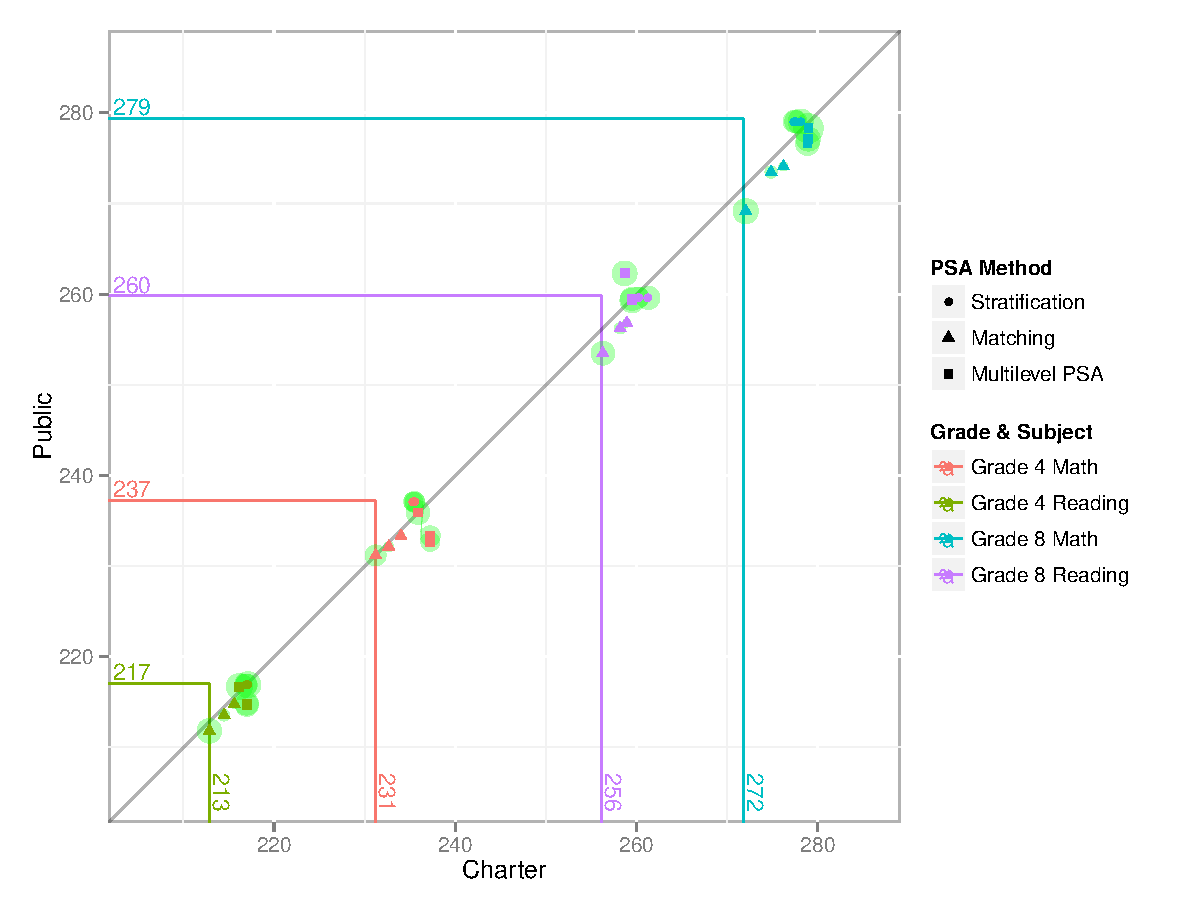
\includegraphics[width=\textwidth]{../Figures2009/OverallScatter.pdf}
\caption{PSA Circle Plot of Adjusted Means}
\label{fig:overallcirc}
\end{center}
\end{figure}



\begin{figure}[ht]
\begin{center}
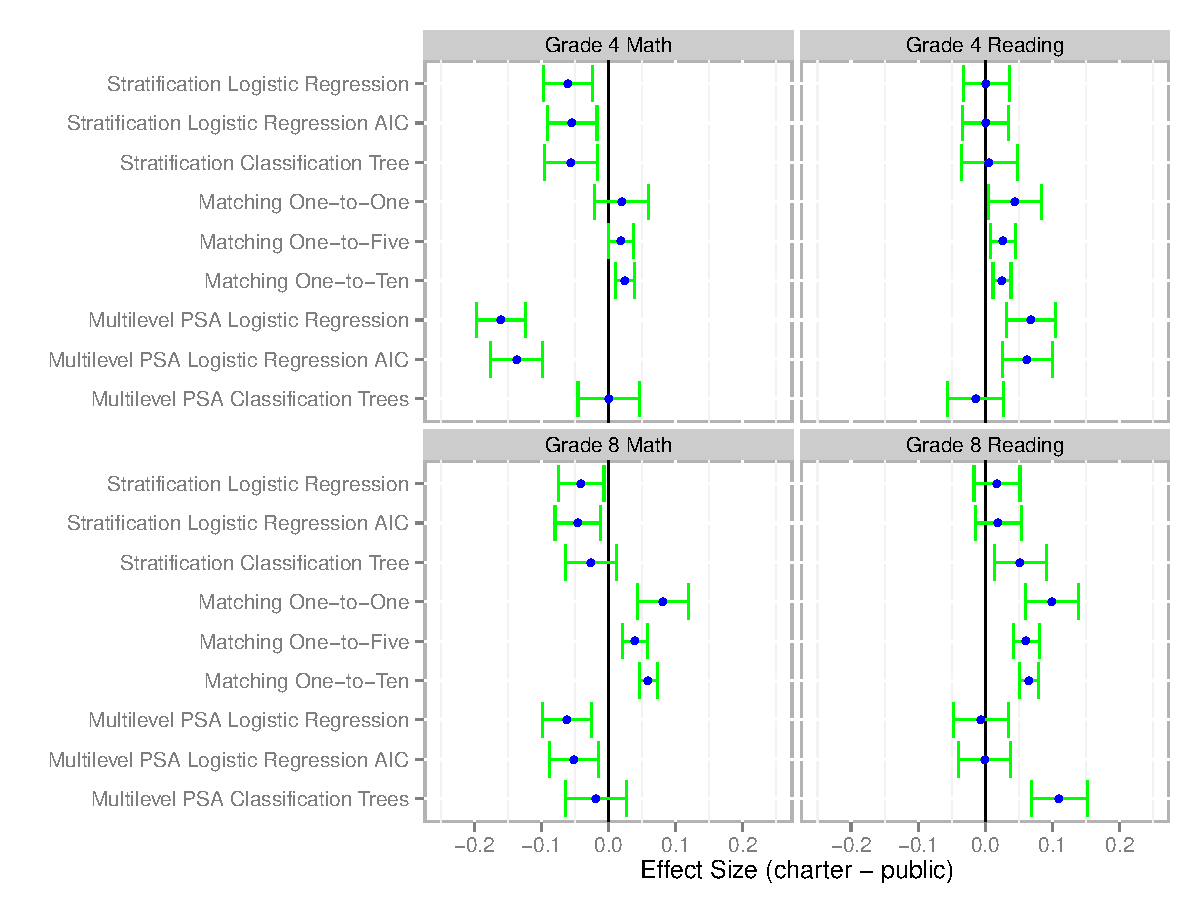
\includegraphics[width=\textwidth]{../Figures2009/Overall.pdf}
\caption{Overall Differences in Effect Size}
\label{fig:overalldiff}
\end{center}
\end{figure}


% latex table generated in R 3.0.1 by xtable 1.7-1 package
% Thu Jun 20 12:52:33 2013
\begin{table}[ht]
\centering
\caption{Summary of overall propensity score results} 
\begin{tabular}{lrrrrr}
  \hline Method & Charter & Public & ATE & \multicolumn{2}{c}{95\% CI} \\   \hline & \multicolumn{5}{c}{Grade 4 Math} \\ \cline{2-6} Stratification Logistic Regression & 235.37 & 237.09 & -0.06 & -2.77 & -0.68 \\ 
  Stratification Logistic Regression AIC & 235.55 & 237.09 & -0.05 & -2.59 & -0.49 \\ 
  Stratification Classification Tree & 235.48 & 237.09 & -0.06 & -2.74 & -0.47 \\ 
  Matching One-to-One & 231.22 & 231.18 & 0.00 & -1.12 & 1.20 \\ 
  Matching One-to-Five & 232.67 & 232.14 & 0.02 & -0.01 & 1.07 \\ 
  Matching One-to-Ten & 234.02 & 233.33 & 0.02 & 0.29 & 1.09 \\ 
  Multilevel PSA Logistic Regression & 237.24 & 232.67 & -0.16 & -3.53 & -5.60 \\ 
  Multilevel PSA Logistic Regression AIC & 237.24 & 233.33 & -0.14 & -2.80 & -5.01 \\ 
  Multilevel PSA Classification Trees & 235.90 & 235.91 & 0.00 & 1.32 & -1.30 \\ 
    \hline & \multicolumn{5}{c}{Grade 4 Reading} \\ \cline{2-6} Stratification Logistic Regression & 216.96 & 216.92 & 0.00 & -1.13 & 1.23 \\ 
  Stratification Logistic Regression AIC & 216.92 & 216.92 & 0.00 & -1.17 & 1.17 \\ 
  Stratification Classification Tree & 217.12 & 216.92 & 0.01 & -1.23 & 1.63 \\ 
  Matching One-to-One & 212.88 & 211.82 & 0.03 & -0.30 & 2.41 \\ 
  Matching One-to-Five & 214.51 & 213.54 & 0.03 & 0.33 & 1.60 \\ 
  Matching One-to-Ten & 215.63 & 214.75 & 0.03 & 0.42 & 1.35 \\ 
  Multilevel PSA Logistic Regression & 217.01 & 214.69 & -0.07 & -1.07 & -3.58 \\ 
  Multilevel PSA Logistic Regression AIC & 216.99 & 214.85 & -0.06 & -0.86 & -3.42 \\ 
  Multilevel PSA Classification Trees & 216.19 & 216.71 & 0.01 & 1.95 & -0.93 \\ 
    \hline & \multicolumn{5}{c}{Grade 8 Math} \\ \cline{2-6} Stratification Logistic Regression & 277.58 & 279.05 & -0.04 & -2.69 & -0.25 \\ 
  Stratification Logistic Regression AIC & 277.41 & 279.06 & -0.05 & -2.86 & -0.43 \\ 
  Stratification Classification Tree & 278.11 & 279.04 & -0.03 & -2.31 & 0.44 \\ 
  Matching One-to-One & 272.05 & 269.16 & 0.08 & 1.51 & 4.28 \\ 
  Matching One-to-Five & 274.85 & 273.46 & 0.04 & 0.72 & 2.06 \\ 
  Matching One-to-Ten & 276.21 & 274.08 & 0.06 & 1.63 & 2.62 \\ 
  Multilevel PSA Logistic Regression & 278.86 & 276.63 & -0.06 & -0.92 & -3.54 \\ 
  Multilevel PSA Logistic Regression AIC & 278.95 & 277.11 & -0.05 & -0.52 & -3.16 \\ 
  Multilevel PSA Classification Trees & 278.98 & 278.30 & -0.02 & 0.94 & -2.30 \\ 
    \hline & \multicolumn{5}{c}{Grade 8 Reading} \\ \cline{2-6} Stratification Logistic Regression & 260.20 & 259.63 & 0.02 & -0.55 & 1.69 \\ 
  Stratification Logistic Regression AIC & 260.25 & 259.63 & 0.02 & -0.49 & 1.74 \\ 
  Stratification Classification Tree & 261.30 & 259.60 & 0.05 & 0.43 & 2.97 \\ 
  Matching One-to-One & 256.29 & 253.48 & 0.09 & 1.51 & 4.12 \\ 
  Matching One-to-Five & 258.19 & 256.24 & 0.06 & 1.33 & 2.58 \\ 
  Matching One-to-Ten & 258.93 & 256.82 & 0.06 & 1.65 & 2.57 \\ 
  Multilevel PSA Logistic Regression & 259.51 & 259.30 & -0.01 & 1.13 & -1.55 \\ 
  Multilevel PSA Logistic Regression AIC & 259.52 & 259.49 & -0.00 & 1.24 & -1.31 \\ 
  Multilevel PSA Classification Trees & 258.70 & 262.29 & 0.11 & 4.96 & 2.23 \\ 
   \hline
\end{tabular}
\label{tab:overall}
\end{table}



%==================== CHAPTER 5 ====================================================================
\cleardoublepage
\section{Chapter 5: Discussion}


Given the significant difference in sample \textit{n}'s for charter and public schools (i.e. there are as much as three to four orders of magnitude more public schools students available in the NAEP data sets), it is expected that there would be public school students who would not have a counterpart from the charter school group. However, the relatively high percentage of public schools students who do not have a charter school counterpart (as much as 35\%) suggest that there may be imbalance between the two groups as a whole. That is, although reasonable balance was achieved with regard to the individual strata where comparisons are made, the overall sample imbalance, as evidenced by the unmatched public school students, suggests that public schools serve a more heterogeneous population.


%==================== REFERENCES ====================================================================
\cleardoublepage
\bibliographystyle{apacite}
\bibliography{Bibliography}

\newpage

%==================== Appendices ====================================================================
\cleardoublepage
\addcontentsline{toc}{section}{Appendices}
\appendix

%==================== Appendix A ====================================================================
\renewcommand{\thefootnote}{\fnsymbol{footnote}}% Change the footnote style to lowercase letters
\addcontentsline{toc}{subsection}{Appendix A: Charter School \& Student Enrollment by State}
\subsection*{Appendix A\\Charter Schools \& Student Enrollment by State}
\label{appendixCharterStats}
\begin{center} \begin{singlespace}
\begin{longtable}{lrrrrrrr}
\caption[Charter Schools \& Student Enrollment by State]{Charter Schools \& Student Enrollment by State} \\
\thickline
      & Law     & \multicolumn{3}{c}{Totals for Charter Schools\tabfnm{b}}              & & \multicolumn{2}{c}{NAEP Students}\\
\cline{3-5} \cline{7-8}
State & Enacted & Operating & Closed & Students & & Charters & Publics\\
\hline
\endfirsthead
\multicolumn{8}{l}{Charter Schools \& Student Enrollment by State (cont.)}\\
\hline
      & Law     & \multicolumn{3}{c}{Totals for Charter Schools\tabfnm{b}}              & & \multicolumn{2}{c}{NAEP Students}\\
\cline{3-5} \cline{7-8}
State & Enacted & Operating & Closed & Students & & Charters & Publics\\
\hline
\endhead
\hline 
\endfoot
\thickline
\endlastfoot
Alabama\tabfnm{a}       &      & 0   & 0   & 0       & &   0 & 2759\\
Alaska                  & 1995 & 26  & 5   & 5,198   & &  69 & 2517\\
Arizona                 & 1994 & 510 & 96  & 119,903 & &  99 & 2674\\
Arkansas                & 1995 & 25  & 6   & 6,750   & &  30 & 2407\\
California              & 1992 & 802 & 103 & 316,468 & & 417 & 7803\\
Colorado                & 1993 & 151 & 10  & 54,497  & & 108 & 2598\\
Connecticut             & 1996 & 21  & 5   & 3,932   & &   0 & 2531\\
Delaware                & 1995 & 21  & 2   & 8,740   & & 180 & 2641\\
Washington DC           & 1996 & 93  & 16  & 25,385  & & 652 & 1336\\
Florida                 & 1996 & 382 & 82  & 108,382 & & 175 & 3876\\
Georgia                 & 1993 & 83  & 5   & 40,807  & &  64 & 3465\\
Hawaii                  & 1994 & 32  & 0   & 7,317   & & 132 & 2605\\
Idaho                   & 1998 & 32  & 1   & 10,492  & &  59 & 2784\\
Illinois                & 1996 & 74  & 8   & 27,683  & &  33 & 4015\\
Indiana                 & 2001 & 50  & 2   & 12,631  & &  11 & 2720\\
Iowa                    & 2002 & 10  & 0   & 1,462   & &   0 & 2839\\
Kansas                  & 1994 & 40  & 10  & 3,361   & &  17 & 2726\\
Kentucky\tabfnm{a}      &      & 0   & 0   & 0       & &   0 & 2696\\
Louisiana               & 1995 & 66  & 10  & 23,634  & &  97 & 2264\\
Maine\tabfnm{a}         &      & 0   & 0   & 0       & &   0 & 2658\\
Maryland                & 2003 & 34  & 2   & 7,301   & &   6 & 2825\\
Massachusetts           & 1993 & 64  & 6   & 23,905  & &  56 & 3667\\
Michigan                & 1993 & 250 & 27  & 94,092  & & 134 & 2480\\
Minnesota               & 1991 & 159 & 29  & 28,371  & &  16 & 2875\\
Mississippi             & 1997 & 1   & 0   & 367     & &   0 & 2613\\
Missouri                & 1998 & 39  & 5   & 13,125  & &  38 & 2771\\
Montana\tabfnm{a}       &      & 0   & 0   & 0       & &   0 & 2581\\
Nebraska\tabfnm{a}      &      & 0   & 0   & 0       & &   0 & 2688\\
Nevada                  & 1997 & 26  & 7   & 7,295   & &   0 & 2662\\
New Hampshire           & 1995 & 11  & 2   & 1,212   & &   0 & 2803\\
New Jersey              & 1996 & 64  & 19  & 17,986  & &   0 & 2813\\
New Mexico              & 1993 & 70  & 3   & 11,426  & &  54 & 2722\\
New York                & 1998 & 118 & 10  & 32,602  & &  16 & 3745\\
North Carolina          & 1996 & 103 & 32  & 30,445  & &  72 & 4090\\
North Dakota\tabfnm{a}  &      & 0   & 0   & 0       & &   0 & 2307\\
Ohio                    & 1997 & 293 & 48  & 94,171  & &  45 & 3746\\
Oklahoma                & 1999 & 14  & 1   & 4,770   & &   0 & 2612\\
Oregon                  & 1999 & 93  & 8   & 13,612  & &  41 & 2626\\
Pennsylvania            & 1997 & 133 & 12  & 61,823  & &  64 & 2709\\
Rhode Island            & 1995 & 11  & 0   & 2,894   & &  30 & 2621\\
South Carolina          & 1996 & 36  & 10  & 8,705   & &  16 & 2697\\
South Dakota\tabfnm{a}  &      & 0   & 0   & 0       & &   0 & 2889\\
Tennessee               & 2002 & 14  & 1   & 2,585   & &  54 & 2815\\
Texas                   & 1995 & 331 & 33  & 108,541 & & 199 & 7070\\
Utah                    & 1998 & 68  & 1   & 23,233  & &  38 & 2722\\
Vermont\tabfnm{a}       &      & 0   & 0   & 0       & &   0 & 2003\\
Virginia                & 1998 & 4   & 3   & 275     & &   0 & 2848\\
Washington\tabfnm{a}    &      & 0   & 0   & 0       & &   0 & 2968\\
West Virginia\tabfnm{a} &      & 0   & 0   & 0       & &   0 & 2831\\
Wisconsin               & 1993 & 221 & 37  & 41,799  & & 114 & 2592\\
Wyoming                 & 1995 & 3   & 0   & 244     & &   0 & 1897\\
\hline
Total                   &      & 4,578 & 657 & 1,407,421 & & 3,164 & 156,963 \\
\end{longtable}
\tabfnt{a}{State currently does not have a charter school law.}
\tabfnt{b}{Source: \citeA{cernumbers}}
\end{singlespace} \end{center}
\renewcommand{\thefootnote}{\arabic{footnote}}% Reset the footnotes back to numbers


%==================== Appendix B ====================================================================
\newpage
\addcontentsline{toc}{subsection}{Appendix B: Thematic Map of Number of Charter Schools in the United States}
\subsection*{Appendix B\\Thematic Map of Number of Charter Schools by State in 2008}
\label{appendixMap}
\begin{figure}[h]
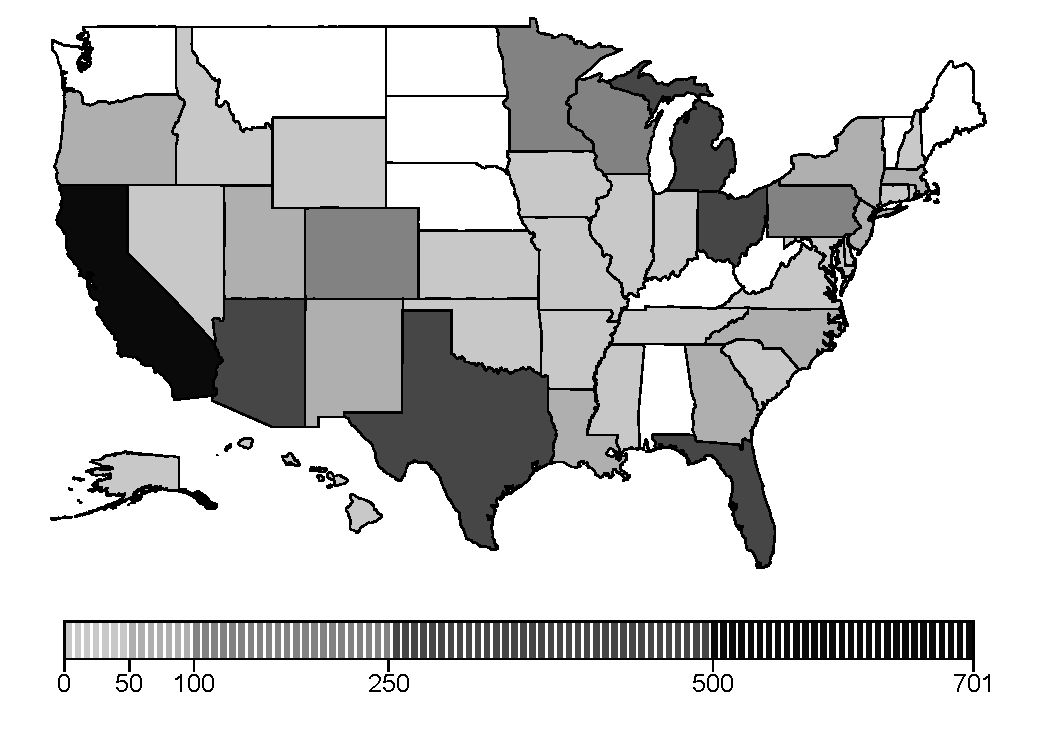
\includegraphics[width=\textwidth]{../Figures/CharterMap.pdf}
\caption{Thematic Map of Number of Charter Schools by State in 2008}
\label{fig:charterMap}
\end{figure}

%==================== Appendix C ====================================================================

%==================== Appendix D ====================================================================
\newpage
\addcontentsline{toc}{subsection}{Appendix D: Descriptive Statistics}
\subsection*{Appendix D\\Descriptive Statistics}
\label{appendixDescriptives}

\begin{singlespace}

\input{../Tables2009/g4Math-desc.tex} \clearpage
% latex table generated in R 3.0.0 by xtable 1.7-1 package
% Fri May 31 15:00:30 2013
\begin{sidewaystable}[ht]
\centering
\caption{Grade 4 Math Unadjusted NAEP Score} 
\label{tab:g4math-unadjscore}
\begin{tabular}{lrrrrrr@{\extracolsep{10pt}}rrrrrr}
  \hline & \multicolumn{6}{c}{Charter Schools} & \multicolumn{6}{c}{Public Schools} \\ \cline{2-7} \cline{8-13} & n & mean & sd & median & min & max & n & mean & sd & median & min & max \\ 
  \hline
Overall & 3625 & 231.93 & 28.19 & 232.18 & 136.95 & 310.45 & 159338 & 238.34 & 27.71 & 239.71 & 117.69 & 334.07 \\ 
  Alaska & 102 & 247.41 & 24.64 & 248.79 & 183.80 & 296.82 & 2496 & 238.50 & 28.87 & 240.91 & 133.70 & 314.90 \\ 
  Arkansas & 226 & 229.38 & 29.27 & 230.22 & 145.74 & 294.08 & 2836 & 228.66 & 29.47 & 229.71 & 142.09 & 324.86 \\ 
  Canal zone & 170 & 223.41 & 26.86 & 221.21 & 152.40 & 290.14 & 7241 & 227.05 & 30.42 & 227.52 & 127.08 & 330.95 \\ 
  Connecticut & 132 & 250.45 & 28.67 & 256.63 & 148.19 & 308.90 & 2550 & 242.34 & 28.39 & 244.89 & 130.83 & 317.99 \\ 
  D.C. & 512 & 217.48 & 26.97 & 215.26 & 146.95 & 306.62 & 1282 & 219.99 & 32.15 & 219.20 & 133.26 & 317.28 \\ 
  Florida & 195 & 240.20 & 26.34 & 238.76 & 168.45 & 294.30 & 2586 & 239.42 & 24.64 & 239.68 & 159.44 & 316.57 \\ 
  Idaho & 166 & 241.09 & 24.28 & 244.36 & 175.09 & 293.17 & 4531 & 239.76 & 24.97 & 240.17 & 147.51 & 324.61 \\ 
  Illinois & 164 & 241.86 & 25.56 & 244.89 & 183.18 & 310.45 & 3865 & 232.69 & 28.18 & 232.54 & 140.58 & 316.17 \\ 
  Iowa &  57 & 230.95 & 26.26 & 234.88 & 146.85 & 273.46 & 2695 & 236.28 & 31.24 & 239.72 & 127.32 & 314.05 \\ 
  Kansas &  60 & 255.08 & 20.79 & 255.56 & 183.42 & 300.83 & 3024 & 240.97 & 24.84 & 242.25 & 139.84 & 314.77 \\ 
  Kentucky &  78 & 229.74 & 27.71 & 231.49 & 147.64 & 295.55 & 4059 & 232.94 & 29.83 & 233.75 & 117.69 & 318.75 \\ 
  Michigan &  65 & 230.80 & 16.68 & 230.98 & 197.30 & 279.19 & 2830 & 229.16 & 24.90 & 229.32 & 144.26 & 308.71 \\ 
  Mississippi & 141 & 219.12 & 26.52 & 217.25 & 164.93 & 293.18 & 3249 & 239.22 & 27.40 & 238.06 & 148.45 & 318.09 \\ 
  Missouri &  52 & 229.29 & 22.62 & 226.30 & 179.65 & 284.75 & 3615 & 248.36 & 25.63 & 249.08 & 145.76 & 317.96 \\ 
  Montana & 215 & 218.06 & 29.43 & 216.04 & 136.95 & 288.98 & 3204 & 229.38 & 31.66 & 231.15 & 128.36 & 318.70 \\ 
  Nebraska & 109 & 247.68 & 26.51 & 248.08 & 188.30 & 302.32 & 3204 & 248.59 & 27.03 & 251.09 & 150.58 & 323.00 \\ 
  New York &  72 & 231.01 & 31.20 & 229.16 & 162.07 & 303.29 & 2977 & 234.90 & 25.81 & 236.10 & 137.78 & 303.75 \\ 
  North Dakota &  74 & 224.15 & 23.57 & 223.48 & 179.04 & 284.71 & 2780 & 247.30 & 26.13 & 249.06 & 155.28 & 325.63 \\ 
  Oklahoma &  60 & 229.73 & 21.88 & 230.70 & 189.84 & 269.90 & 3997 & 239.50 & 26.83 & 240.45 & 145.65 & 315.10 \\ 
  Oregon &  96 & 249.72 & 19.40 & 250.68 & 206.39 & 290.68 & 4320 & 243.07 & 26.92 & 243.12 & 130.47 & 323.33 \\ 
  Rhode Island & 124 & 218.15 & 22.02 & 217.22 & 159.99 & 269.17 & 3324 & 237.62 & 29.58 & 239.43 & 126.61 & 319.60 \\ 
  Utah &  79 & 230.94 & 23.07 & 227.57 & 185.38 & 297.38 & 2404 & 239.08 & 28.41 & 241.89 & 136.10 & 307.88 \\ 
  Washington &  91 & 231.23 & 20.75 & 229.44 & 166.83 & 278.23 & 6193 & 238.97 & 24.48 & 239.19 & 139.25 & 317.06 \\ 
  West Virginia & 197 & 247.20 & 25.79 & 250.06 & 164.01 & 305.53 & 3145 & 239.22 & 28.47 & 241.50 & 130.38 & 319.46 \\ 
  DoDEA/DDESS & 136 & 229.43 & 26.14 & 226.78 & 178.41 & 289.56 & 3694 & 237.95 & 29.14 & 239.24 & 134.42 & 320.51 \\ 
   \hline
\end{tabular}
\end{sidewaystable}
 \clearpage

% latex table generated in R 3.0.1 by xtable 1.7-1 package
% Wed Jun 19 20:22:03 2013
\begin{longtable}{lrr@{\extracolsep{10pt}}rr}
\caption{Grade 4 Reading Descriptive Statistics} \\ 
   \thickline & \multicolumn{2}{c}{Traditional} & \multicolumn{2}{c}{Charter} \\  \endfirsthead \multicolumn{5}{l}{{...continued from previous page}}\\ \hline & \multicolumn{2}{c}{Charter} & \multicolumn{2}{c}{Traditional}  \\ \hline \endhead \thickline \multicolumn{5}{r}{continued on next page...} \\ \endfoot \multicolumn{5}{c}{} \\ \endlastfoot  \pagebreak[2] \hline \multicolumn{5}{c}{Race/ethnicity from school records (raw data)} \\ \cline{1-5} White & 96992 & 58\% & 1343 & 34\% \\ 
  Black & 29127 & 17\% & 1636 & 42\% \\ 
  Hispanic & 28133 & 17\% & 705 & 18\% \\ 
  Asian Amer/Pacif Is & 8114 & 5\% & 162 & 4\% \\ 
  Amer Ind/Alaska Nat & 3898 & 2\% &  49 & 1\% \\ 
  Other & 2333 & 1\% &  41 & 1\% \\ 
  Unknown &   0 & 0\% &   0 & 0\% \\ 
   \pagebreak[2] \hline \multicolumn{5}{c}{Natl School Lunch Prog eligibility (3 categories)} \\ \cline{1-5} Eligible & 82354 & 49\% & 2223 & 56\% \\ 
  Not eligible & 85304 & 51\% & 1528 & 39\% \\ 
  Info not available & 939 & 1\% & 185 & 5\% \\ 
  Unknown &   0 & 0\% &   0 & 0\% \\ 
   \pagebreak[2] \hline \multicolumn{5}{c}{Student has Individualized Education Plan} \\ \cline{1-5} Yes, IEP & 16579 & 10\% & 307 & 8\% \\ 
  Yes, 504 plan & 1385 & 1\% &  29 & 1\% \\ 
  Yes, 504 in process &   0 & 0\% &   0 & 0\% \\ 
  Not IEP & 150596 & 89\% & 3600 & 91\% \\ 
  Omitted &   0 & 0\% &   0 & 0\% \\ 
  Unknown &  37 & 0\% &   0 & 0\% \\ 
   \pagebreak[2] \hline \multicolumn{5}{c}{Student classified Eng Lang Learner (3 categories)} \\ \cline{1-5} Yes & 12095 & 7\% & 285 & 7\% \\ 
  No & 153110 & 91\% & 3569 & 91\% \\ 
  Formerly ELL & 3357 & 2\% &  82 & 2\% \\ 
  Omitted &   0 & 0\% &   0 & 0\% \\ 
  Unknown &  35 & 0\% &   0 & 0\% \\ 
   \pagebreak[2] \hline \multicolumn{5}{c}{Gender} \\ \cline{1-5} Male & 85214 & 51\% & 1960 & 50\% \\ 
  Female & 83383 & 49\% & 1976 & 50\% \\ 
  Unknown &   0 & 0\% &   0 & 0\% \\ 
   \pagebreak[2] \hline \multicolumn{5}{c}{Student classified as having a disability (504)} \\ \cline{1-5} Student with disabi & 17964 & 11\% & 336 & 9\% \\ 
  Not student with di & 150596 & 89\% & 3600 & 91\% \\ 
  Omitted &  37 & 0\% &   0 & 0\% \\ 
  Unknown &   0 & 0\% &   0 & 0\% \\ 
   \pagebreak[2] \hline \multicolumn{5}{c}{Student classified SD or ELL} \\ \cline{1-5} Student with disabi & 16722 & 10\% & 314 & 8\% \\ 
  English language le & 10853 & 6\% & 263 & 7\% \\ 
  Both SD and ELL & 1242 & 1\% &  22 & 1\% \\ 
  Neither SD nor ELL & 139727 & 83\% & 3337 & 85\% \\ 
  Unknown &  53 & 0\% &   0 & 0\% \\ 
   \pagebreak[2] \hline \multicolumn{5}{c}{Newspaper in home} \\ \cline{1-5} Yes & 47839 & 28\% & 1141 & 29\% \\ 
  No & 59247 & 35\% & 1327 & 34\% \\ 
  I Don't Know & 58294 & 35\% & 1343 & 34\% \\ 
  Omitted & 3205 & 2\% & 125 & 3\% \\ 
  Multiple &  12 & 0\% &   0 & 0\% \\ 
  Unknown &   0 & 0\% &   0 & 0\% \\ 
   \pagebreak[2] \hline \multicolumn{5}{c}{Magazines in home} \\ \cline{1-5} Yes & 95695 & 57\% & 2225 & 57\% \\ 
  No & 40167 & 24\% & 911 & 23\% \\ 
  I Don't Know & 29309 & 17\% & 667 & 17\% \\ 
  Omitted & 3404 & 2\% & 133 & 3\% \\ 
  Multiple &  22 & 0\% &   0 & 0\% \\ 
  Unknown &   0 & 0\% &   0 & 0\% \\ 
   \pagebreak[2] \hline \multicolumn{5}{c}{Books in home} \\ \cline{1-5} 0-10 books & 19634 & 12\% & 434 & 11\% \\ 
  11-25 books & 35306 & 21\% & 901 & 23\% \\ 
  26-100 books & 56725 & 34\% & 1217 & 31\% \\ 
  More than 100 books & 53526 & 32\% & 1258 & 32\% \\ 
  Omitted & 3359 & 2\% & 126 & 3\% \\ 
  Multiple &  47 & 0\% &   0 & 0\% \\ 
  Unknown &   0 & 0\% &   0 & 0\% \\ 
   \pagebreak[2] \hline \multicolumn{5}{c}{Computer in home} \\ \cline{1-5} Yes & 144162 & 86\% & 3362 & 85\% \\ 
  No & 20419 & 12\% & 428 & 11\% \\ 
  Omitted & 3999 & 2\% & 146 & 4\% \\ 
  Multiple &  17 & 0\% &   0 & 0\% \\ 
  Unknown &   0 & 0\% &   0 & 0\% \\ 
   \pagebreak[2] \hline \multicolumn{5}{c}{Encyclopedia in home} \\ \cline{1-5} Yes & 85818 & 51\% & 2035 & 52\% \\ 
  No & 25320 & 15\% & 544 & 14\% \\ 
  I Don't Know & 54087 & 32\% & 1229 & 31\% \\ 
  Omitted & 3350 & 2\% & 128 & 3\% \\ 
  Multiple &  22 & 0\% &   0 & 0\% \\ 
  Unknown &   0 & 0\% &   0 & 0\% \\ 
   \pagebreak[2] \hline \multicolumn{5}{c}{Pages read in school and for homework} \\ \cline{1-5} 5 or fewer & 34944 & 21\% & 912 & 23\% \\ 
  6-10 & 30880 & 18\% & 746 & 19\% \\ 
  11-15 & 23139 & 14\% & 449 & 11\% \\ 
  16-20 & 23805 & 14\% & 529 & 13\% \\ 
  More than 20 & 52313 & 31\% & 1167 & 30\% \\ 
  Omitted & 3450 & 2\% & 129 & 3\% \\ 
  Multiple &  66 & 0\% &   4 & 0\% \\ 
  Unknown &   0 & 0\% &   0 & 0\% \\ 
   \pagebreak[2] \hline \multicolumn{5}{c}{Talk about studies at home} \\ \cline{1-5} Never or hardly eve & 29602 & 18\% & 648 & 16\% \\ 
  Every few weeks & 22498 & 13\% & 475 & 12\% \\ 
  About once a week & 19884 & 12\% & 429 & 11\% \\ 
  2-3 times a week & 33893 & 20\% & 687 & 17\% \\ 
  Every day & 59212 & 35\% & 1566 & 40\% \\ 
  Omitted & 3465 & 2\% & 129 & 3\% \\ 
  Multiple &  43 & 0\% &   2 & 0\% \\ 
  Unknown &   0 & 0\% &   0 & 0\% \\ 
   \pagebreak[2] \hline \multicolumn{5}{c}{Days absent from school last month} \\ \cline{1-5} None & 84418 & 50\% & 1838 & 47\% \\ 
  1-2 days & 49650 & 29\% & 1177 & 30\% \\ 
  3-4 days & 19327 & 11\% & 474 & 12\% \\ 
  5-10 days & 7608 & 5\% & 208 & 5\% \\ 
  More than 10 days & 4136 & 2\% & 109 & 3\% \\ 
  Omitted & 3396 & 2\% & 128 & 3\% \\ 
  Multiple &  62 & 0\% &   2 & 0\% \\ 
  Unknown &   0 & 0\% &   0 & 0\% \\ 
   \pagebreak[2] \hline \multicolumn{5}{c}{Language other than English spoken in home} \\ \cline{1-5} Never & 90390 & 54\% & 1798 & 46\% \\ 
  Once in a while & 36078 & 21\% & 901 & 23\% \\ 
  Half the time & 12161 & 7\% & 362 & 9\% \\ 
  All or most of time & 26507 & 16\% & 743 & 19\% \\ 
  Omitted & 3412 & 2\% & 129 & 3\% \\ 
  Multiple &  49 & 0\% &   3 & 0\% \\ 
  Unknown &   0 & 0\% &   0 & 0\% \\ 
   \pagebreak[2] \hline \multicolumn{5}{c}{Learn a lot when reading books} \\ \cline{1-5} Never or hardly eve & 8448 & 5\% & 185 & 5\% \\ 
  Sometimes & 59897 & 36\% & 1331 & 34\% \\ 
  Often & 50052 & 30\% & 1076 & 27\% \\ 
  Always or almost & 46493 & 28\% & 1201 & 31\% \\ 
  Omitted & 3687 & 2\% & 142 & 4\% \\ 
  Multiple &  20 & 0\% &   1 & 0\% \\ 
  Unknown &   0 & 0\% &   0 & 0\% \\ 
   \pagebreak[2] \hline \multicolumn{5}{c}{Reading is a favorite subject} \\ \cline{1-5} Never or hardly eve & 25581 & 15\% & 611 & 16\% \\ 
  Sometimes & 60476 & 36\% & 1409 & 36\% \\ 
  Often & 36703 & 22\% & 783 & 20\% \\ 
  Always or almost & 41959 & 25\% & 987 & 25\% \\ 
  Omitted & 3855 & 2\% & 146 & 4\% \\ 
  Multiple &  23 & 0\% &   0 & 0\% \\ 
  Unknown &   0 & 0\% &   0 & 0\% \\ 
   \pagebreak[2] \hline \multicolumn{5}{c}{Do reading at after-school or tutoring program} \\ \cline{1-5} Yes & 60364 & 36\% & 1718 & 44\% \\ 
  No & 102803 & 61\% & 2029 & 52\% \\ 
  Omitted & 5387 & 3\% & 189 & 5\% \\ 
  Multiple &  43 & 0\% &   0 & 0\% \\ 
  Unknown &   0 & 0\% &   0 & 0\% \\ 
   \pagebreak[2] \hline \multicolumn{5}{c}{Go to book clubs, competitions, fairs for reading} \\ \cline{1-5} Yes & 49006 & 29\% & 1255 & 32\% \\ 
  No & 113968 & 68\% & 2491 & 63\% \\ 
  Omitted & 5592 & 3\% & 189 & 5\% \\ 
  Multiple &  31 & 0\% &   1 & 0\% \\ 
  Unknown &   0 & 0\% &   0 & 0\% \\ 
   \pagebreak[2] \hline \multicolumn{5}{c}{Read for fun on own} \\ \cline{1-5} Never or hardly eve & 25028 & 15\% & 584 & 15\% \\ 
  Once or twice/month & 24696 & 15\% & 569 & 14\% \\ 
  1-2 times a week & 41186 & 24\% & 923 & 23\% \\ 
  Almost every day & 72670 & 43\% & 1677 & 43\% \\ 
  Omitted & 4984 & 3\% & 182 & 5\% \\ 
  Multiple &  33 & 0\% &   1 & 0\% \\ 
  Unknown &   0 & 0\% &   0 & 0\% \\ 
   \pagebreak[2] \hline \multicolumn{5}{c}{Talk with friends about what you read} \\ \cline{1-5} Never or hardly eve & 46333 & 27\% & 997 & 25\% \\ 
  Once or twice/month & 34554 & 20\% & 739 & 19\% \\ 
  1-2 times a week & 43383 & 26\% & 943 & 24\% \\ 
  Almost every day & 40113 & 24\% & 1106 & 28\% \\ 
  Omitted & 4180 & 2\% & 150 & 4\% \\ 
  Multiple &  34 & 0\% &   1 & 0\% \\ 
  Unknown &   0 & 0\% &   0 & 0\% \\ 
   \pagebreak[2] \hline \multicolumn{5}{c}{Read a book you chose yourself} \\ \cline{1-5} Never or hardly eve & 22712 & 13\% & 593 & 15\% \\ 
  Sometimes & 40804 & 24\% & 1009 & 26\% \\ 
  Often & 42467 & 25\% & 932 & 24\% \\ 
  Always or almost & 56171 & 33\% & 1196 & 30\% \\ 
  Omitted & 6413 & 4\% & 205 & 5\% \\ 
  Multiple &  30 & 0\% &   1 & 0\% \\ 
  Unknown &   0 & 0\% &   0 & 0\% \\ 
  \hline
\label{tab:g4Reading-desc}
\end{longtable}
 \clearpage
% latex table generated in R 3.0.0 by xtable 1.7-1 package
% Fri May 31 15:00:31 2013
\begin{sidewaystable}[ht]
\centering
\caption{Grade 4 Reading Unadjusted NAEP Score} 
\label{tab:g4read-unadjscore}
\begin{tabular}{lrrrrrr@{\extracolsep{10pt}}rrrrrr}
  \hline & \multicolumn{6}{c}{Charter Schools} & \multicolumn{6}{c}{Public Schools} \\ \cline{2-7} \cline{8-13} & n & mean & sd & median & min & max & n & mean & sd & median & min & max \\ 
  \hline
Overall & 3936 & 213.26 & 32.94 & 215.22 & 92.27 & 302.97 & 168597 & 218.76 & 33.66 & 221.79 & 14.71 & 330.96 \\ 
  Alaska & 117 & 226.06 & 33.86 & 233.08 & 101.93 & 278.72 & 2666 & 214.43 & 36.60 & 219.70 & 78.50 & 302.46 \\ 
  Arkansas & 242 & 213.15 & 34.22 & 216.30 & 105.63 & 294.52 & 2943 & 208.58 & 38.27 & 212.92 & 14.71 & 319.32 \\ 
  Canal zone & 183 & 196.96 & 35.30 & 194.82 & 92.27 & 286.62 & 7822 & 204.44 & 35.95 & 206.11 & 51.07 & 318.34 \\ 
  Connecticut & 143 & 229.69 & 33.61 & 235.33 & 124.55 & 291.85 & 2777 & 225.49 & 34.52 & 230.29 & 85.98 & 316.87 \\ 
  D.C. & 541 & 198.75 & 31.53 & 199.60 & 102.07 & 280.99 & 1307 & 204.14 & 37.69 & 203.42 & 71.14 & 330.96 \\ 
  Florida & 216 & 222.89 & 27.69 & 223.23 & 152.52 & 293.06 & 2649 & 225.96 & 27.61 & 227.81 & 113.17 & 309.18 \\ 
  Idaho & 185 & 227.25 & 24.58 & 228.11 & 141.86 & 288.14 & 4771 & 224.10 & 29.65 & 226.17 & 97.23 & 312.59 \\ 
  Illinois & 179 & 220.16 & 32.54 & 220.82 & 94.63 & 287.95 & 4056 & 215.07 & 33.27 & 216.54 & 89.20 & 321.26 \\ 
  Iowa &  78 & 215.14 & 36.63 & 222.41 & 96.15 & 289.85 & 2914 & 210.77 & 38.37 & 214.86 & 50.22 & 309.30 \\ 
  Kansas &  72 & 242.29 & 27.73 & 247.02 & 157.89 & 290.30 & 3169 & 220.49 & 31.59 & 224.11 & 73.45 & 294.68 \\ 
  Kentucky &  81 & 204.56 & 33.03 & 206.21 & 134.27 & 276.43 & 4314 & 213.09 & 36.59 & 216.16 & 82.70 & 322.40 \\ 
  Michigan &  73 & 200.08 & 24.97 & 197.83 & 158.07 & 269.88 & 3079 & 207.87 & 31.56 & 209.30 & 75.54 & 298.16 \\ 
  Mississippi & 152 & 207.05 & 28.29 & 208.95 & 142.04 & 274.30 & 3297 & 220.71 & 32.60 & 220.73 & 109.43 & 322.77 \\ 
  Missouri &  54 & 225.77 & 22.09 & 225.23 & 169.00 & 265.05 & 3894 & 229.30 & 30.48 & 231.56 & 95.48 & 309.48 \\ 
  Montana & 217 & 201.20 & 31.78 & 202.59 & 123.87 & 289.31 & 3487 & 212.74 & 34.23 & 215.29 & 75.67 & 302.63 \\ 
  Nebraska & 109 & 221.06 & 36.91 & 223.34 & 101.89 & 285.11 & 3506 & 222.79 & 34.75 & 227.05 & 58.17 & 316.17 \\ 
  New York &  75 & 215.17 & 29.94 & 216.60 & 134.65 & 278.63 & 3155 & 210.12 & 35.62 & 213.99 & 18.03 & 295.53 \\ 
  North Dakota &  80 & 213.75 & 21.85 & 212.65 & 153.51 & 263.03 & 2805 & 230.06 & 28.90 & 231.41 & 118.16 & 321.05 \\ 
  Oklahoma &  69 & 220.92 & 30.41 & 218.55 & 157.69 & 300.34 & 4162 & 221.95 & 32.22 & 224.25 & 99.34 & 306.82 \\ 
  Oregon & 104 & 226.53 & 26.97 & 227.31 & 148.58 & 287.27 & 4720 & 219.46 & 34.73 & 223.00 & 40.55 & 309.55 \\ 
  Rhode Island & 138 & 196.41 & 31.14 & 196.45 & 112.19 & 273.31 & 3464 & 218.63 & 32.97 & 220.65 & 101.22 & 305.91 \\ 
  South Dakota &  56 & 225.22 & 31.87 & 229.31 & 148.54 & 285.83 & 3027 & 217.79 & 35.12 & 221.68 & 44.79 & 306.49 \\ 
  Tennessee &  59 & 218.66 & 33.26 & 221.67 & 130.12 & 302.97 & 3846 & 216.38 & 36.39 & 218.94 & 45.75 & 316.07 \\ 
  Utah &  85 & 217.99 & 31.30 & 218.14 & 135.33 & 283.96 & 2566 & 222.83 & 34.75 & 226.45 & 49.36 & 310.49 \\ 
  Washington & 100 & 217.52 & 24.77 & 220.63 & 151.32 & 277.02 & 5854 & 216.69 & 30.85 & 216.91 & 91.15 & 318.03 \\ 
  West Virginia & 203 & 228.59 & 27.26 & 231.71 & 137.46 & 287.80 & 3290 & 218.54 & 32.67 & 222.79 & 46.89 & 303.80 \\ 
  DoDEA/DDESS & 153 & 200.04 & 32.60 & 198.92 & 123.03 & 273.93 & 3935 & 214.63 & 35.37 & 218.79 & 92.04 & 301.72 \\ 
   \hline
\end{tabular}
\end{sidewaystable}
 \clearpage

% latex table generated in R 3.0.1 by xtable 1.7-1 package
% Wed Jun 19 20:22:07 2013
{\normalsize
\begin{longtable}{lrr@{\extracolsep{10pt}}rr}
\caption{Grade 8 math descriptive statistics} \\ 
   \thickline & \multicolumn{2}{c}{Traditional} & \multicolumn{2}{c}{Charter} \\  \endfirsthead \multicolumn{5}{l}{{...continued from previous page}}\\ \hline & \multicolumn{2}{c}{Charter} & \multicolumn{2}{c}{Traditional}  \\ \hline \endhead \thickline \multicolumn{5}{r}{continued on next page...} \\ \endfoot \multicolumn{5}{c}{} \\ \endlastfoot  \pagebreak[2] \hline \multicolumn{5}{c}{Race/ethnicity from school records (raw data)} \\ \cline{1-5} White & 89701 & 59\% & 1114 & 27\% \\ 
  Black & 26613 & 18\% & 1711 & 41\% \\ 
  Hispanic & 23669 & 16\% & 974 & 24\% \\ 
  Asian Amer/Pacif Is & 7318 & 5\% & 230 & 6\% \\ 
  Amer Ind/Alaska Nat & 3250 & 2\% &  55 & 1\% \\ 
  Other & 1497 & 1\% &  46 & 1\% \\ 
  Unknown &   0 & 0\% &   0 & 0\% \\ 
   \pagebreak[2] \hline \multicolumn{5}{c}{Natl School Lunch Prog eligibility (3 categories)} \\ \cline{1-5} Eligible & 67525 & 44\% & 2358 & 57\% \\ 
  Not eligible & 83452 & 55\% & 1553 & 38\% \\ 
  Info not available & 1071 & 1\% & 219 & 5\% \\ 
  Unknown &   0 & 0\% &   0 & 0\% \\ 
   \pagebreak[2] \hline \multicolumn{5}{c}{Student has Individualized Education Plan} \\ \cline{1-5} Yes, IEP & 14792 & 10\% & 377 & 9\% \\ 
  Yes, 504 plan & 1308 & 1\% &  38 & 1\% \\ 
  Yes, 504 in process &   0 & 0\% &   0 & 0\% \\ 
  Not IEP & 135935 & 89\% & 3715 & 90\% \\ 
  Unknown &  13 & 0\% &   0 & 0\% \\ 
   \pagebreak[2] \hline \multicolumn{5}{c}{Student classified Eng Lang Learner (3 categories)} \\ \cline{1-5} Yes & 6615 & 4\% & 276 & 7\% \\ 
  No & 142006 & 93\% & 3712 & 90\% \\ 
  Formerly ELL & 3404 & 2\% & 140 & 3\% \\ 
  Unknown &  23 & 0\% &   2 & 0\% \\ 
   \pagebreak[2] \hline \multicolumn{5}{c}{Gender} \\ \cline{1-5} Male & 76976 & 51\% & 1996 & 48\% \\ 
  Female & 75072 & 49\% & 2134 & 52\% \\ 
  Unknown &   0 & 0\% &   0 & 0\% \\ 
   \pagebreak[2] \hline \multicolumn{5}{c}{Student classified as having a disability (504)} \\ \cline{1-5} Student with disabi & 16100 & 11\% & 415 & 10\% \\ 
  Not student with di & 135935 & 89\% & 3715 & 90\% \\ 
  Omitted &  13 & 0\% &   0 & 0\% \\ 
  Unknown &   0 & 0\% &   0 & 0\% \\ 
   \pagebreak[2] \hline \multicolumn{5}{c}{Student classified SD or ELL} \\ \cline{1-5} Student with disabi & 15250 & 10\% & 389 & 9\% \\ 
  English language le & 5765 & 4\% & 250 & 6\% \\ 
  Both SD and ELL & 850 & 1\% &  26 & 1\% \\ 
  Neither SD nor ELL & 130158 & 86\% & 3464 & 84\% \\ 
  Unknown &  25 & 0\% &   1 & 0\% \\ 
   \pagebreak[2] \hline \multicolumn{5}{c}{Newspaper in home} \\ \cline{1-5} Yes & 55041 & 36\% & 1501 & 36\% \\ 
  No & 62855 & 41\% & 1740 & 42\% \\ 
  I Don't Know & 31056 & 20\% & 862 & 21\% \\ 
  Omitted & 3068 & 2\% &  27 & 1\% \\ 
  Multiple &  28 & 0\% &   0 & 0\% \\ 
  Unknown &   0 & 0\% &   0 & 0\% \\ 
   \pagebreak[2] \hline \multicolumn{5}{c}{Magazines in home} \\ \cline{1-5} Yes & 92419 & 61\% & 2444 & 59\% \\ 
  No & 40632 & 27\% & 1198 & 29\% \\ 
  I Don't Know & 15801 & 10\% & 456 & 11\% \\ 
  Omitted & 3172 & 2\% &  32 & 1\% \\ 
  Multiple &  24 & 0\% &   0 & 0\% \\ 
  Unknown &   0 & 0\% &   0 & 0\% \\ 
   \pagebreak[2] \hline \multicolumn{5}{c}{Books in home} \\ \cline{1-5} 0-10 books & 21803 & 14\% & 578 & 14\% \\ 
  11-25 books & 32216 & 21\% & 966 & 23\% \\ 
  26-100 books & 51674 & 34\% & 1404 & 34\% \\ 
  More than 100 books & 42985 & 28\% & 1148 & 28\% \\ 
  Omitted & 3318 & 2\% &  34 & 1\% \\ 
  Multiple &  52 & 0\% &   0 & 0\% \\ 
  Unknown &   0 & 0\% &   0 & 0\% \\ 
   \pagebreak[2] \hline \multicolumn{5}{c}{Computer in home} \\ \cline{1-5} Yes & 133737 & 88\% & 3658 & 89\% \\ 
  No & 13012 & 9\% & 386 & 9\% \\ 
  Omitted & 5276 & 3\% &  86 & 2\% \\ 
  Multiple &  23 & 0\% &   0 & 0\% \\ 
  Unknown &   0 & 0\% &   0 & 0\% \\ 
   \pagebreak[2] \hline \multicolumn{5}{c}{Encyclopedia in home} \\ \cline{1-5} Yes & 106692 & 70\% & 3015 & 73\% \\ 
  No & 22181 & 15\% & 571 & 14\% \\ 
  I Don't Know & 19857 & 13\% & 509 & 12\% \\ 
  Omitted & 3290 & 2\% &  35 & 1\% \\ 
  Multiple &  28 & 0\% &   0 & 0\% \\ 
  Unknown &   0 & 0\% &   0 & 0\% \\ 
   \pagebreak[2] \hline \multicolumn{5}{c}{Pages read in school and for homework} \\ \cline{1-5} 5 or fewer & 44700 & 29\% & 1192 & 29\% \\ 
  6-10 & 32989 & 22\% & 928 & 22\% \\ 
  11-15 & 21654 & 14\% & 582 & 14\% \\ 
  16-20 & 17204 & 11\% & 512 & 12\% \\ 
  More than 20 & 31906 & 21\% & 865 & 21\% \\ 
  Omitted & 3486 & 2\% &  46 & 1\% \\ 
  Multiple & 109 & 0\% &   5 & 0\% \\ 
  Unknown &   0 & 0\% &   0 & 0\% \\ 
   \pagebreak[2] \hline \multicolumn{5}{c}{Talk about studies at home} \\ \cline{1-5} Never or hardly eve & 35140 & 23\% & 825 & 20\% \\ 
  Every few weeks & 28163 & 19\% & 776 & 19\% \\ 
  About once a week & 26142 & 17\% & 698 & 17\% \\ 
  2-3 times a week & 31254 & 21\% & 924 & 22\% \\ 
  Every day & 27771 & 18\% & 863 & 21\% \\ 
  Omitted & 3512 & 2\% &  44 & 1\% \\ 
  Multiple &  66 & 0\% &   0 & 0\% \\ 
  Unknown &   0 & 0\% &   0 & 0\% \\ 
   \pagebreak[2] \hline \multicolumn{5}{c}{Days absent from school last month} \\ \cline{1-5} None & 65078 & 43\% & 1692 & 41\% \\ 
  1-2 days & 52510 & 35\% & 1393 & 34\% \\ 
  3-4 days & 20084 & 13\% & 651 & 16\% \\ 
  5-10 days & 7792 & 5\% & 257 & 6\% \\ 
  More than 10 days & 3158 & 2\% & 101 & 2\% \\ 
  Omitted & 3369 & 2\% &  35 & 1\% \\ 
  Multiple &  57 & 0\% &   1 & 0\% \\ 
  Unknown &   0 & 0\% &   0 & 0\% \\ 
   \pagebreak[2] \hline \multicolumn{5}{c}{Mother's education level} \\ \cline{1-5} Did not finish h.s. & 15175 & 10\% & 444 & 11\% \\ 
  Graduated h.s. & 30320 & 20\% & 789 & 19\% \\ 
  Some ed after h.s. & 25294 & 17\% & 752 & 18\% \\ 
  Graduated college & 55231 & 36\% & 1396 & 34\% \\ 
  I Don't Know & 22091 & 15\% & 701 & 17\% \\ 
  Omitted & 3648 & 2\% &  44 & 1\% \\ 
  Multiple & 289 & 0\% &   4 & 0\% \\ 
  Unknown &   0 & 0\% &   0 & 0\% \\ 
   \pagebreak[2] \hline \multicolumn{5}{c}{Father's education level} \\ \cline{1-5} Did not finish h.s. & 15904 & 10\% & 457 & 11\% \\ 
  Graduated h.s. & 30398 & 20\% & 730 & 18\% \\ 
  Some ed after h.s. & 19878 & 13\% & 504 & 12\% \\ 
  Graduated college & 46634 & 31\% & 1115 & 27\% \\ 
  I Don't Know & 35054 & 23\% & 1267 & 31\% \\ 
  Omitted & 3955 & 3\% &  52 & 1\% \\ 
  Multiple & 225 & 0\% &   5 & 0\% \\ 
  Unknown &   0 & 0\% &   0 & 0\% \\ 
   \pagebreak[2] \hline \multicolumn{5}{c}{Language other than English spoken in home} \\ \cline{1-5} Never & 86942 & 57\% & 1938 & 47\% \\ 
  Once in a while & 28690 & 19\% & 860 & 21\% \\ 
  Half the time & 11236 & 7\% & 428 & 10\% \\ 
  All or most of time & 20361 & 13\% & 821 & 20\% \\ 
  Omitted & 4766 & 3\% &  80 & 2\% \\ 
  Multiple &  53 & 0\% &   3 & 0\% \\ 
  Unknown &   0 & 0\% &   0 & 0\% \\ 
   \pagebreak[2] \hline \multicolumn{5}{c}{Do math at after-school or tutoring program} \\ \cline{1-5} Yes & 25981 & 17\% & 1025 & 25\% \\ 
  No & 109053 & 72\% & 2712 & 66\% \\ 
  Omitted & 16955 & 11\% & 393 & 10\% \\ 
  Multiple &  59 & 0\% &   0 & 0\% \\ 
  Unknown &   0 & 0\% &   0 & 0\% \\ 
   \pagebreak[2] \hline \multicolumn{5}{c}{Math work is too easy} \\ \cline{1-5} Never or hardly eve & 25733 & 17\% & 667 & 16\% \\ 
  Sometimes & 79651 & 52\% & 2205 & 53\% \\ 
  Often & 29995 & 20\% & 800 & 19\% \\ 
  Always/almost alway & 11127 & 7\% & 339 & 8\% \\ 
  Omitted & 5343 & 4\% & 111 & 3\% \\ 
  Multiple & 199 & 0\% &   8 & 0\% \\ 
  Unknown &   0 & 0\% &   0 & 0\% \\ 
   \pagebreak[2] \hline \multicolumn{5}{c}{Math work is challenging} \\ \cline{1-5} Never or hardly eve & 17626 & 12\% & 418 & 10\% \\ 
  Sometimes & 64961 & 43\% & 1726 & 42\% \\ 
  Often & 44818 & 29\% & 1298 & 31\% \\ 
  Always/almost alway & 16629 & 11\% & 512 & 12\% \\ 
  Omitted & 7824 & 5\% & 174 & 4\% \\ 
  Multiple & 190 & 0\% &   2 & 0\% \\ 
  Unknown &   0 & 0\% &   0 & 0\% \\ 
   \pagebreak[2] \hline \multicolumn{5}{c}{Math work is engaging and interesting} \\ \cline{1-5} Never or hardly eve & 34020 & 22\% & 756 & 18\% \\ 
  Sometimes & 53378 & 35\% & 1415 & 34\% \\ 
  Often & 38173 & 25\% & 1054 & 26\% \\ 
  Always or almost & 19386 & 13\% & 732 & 18\% \\ 
  Omitted & 7027 & 5\% & 171 & 4\% \\ 
  Multiple &  64 & 0\% &   2 & 0\% \\ 
  Unknown &   0 & 0\% &   0 & 0\% \\ 
   \pagebreak[2] \hline \multicolumn{5}{c}{Math is fun} \\ \cline{1-5} Strongly disagree & 17997 & 12\% & 472 & 11\% \\ 
  Disagree & 49601 & 33\% & 1262 & 31\% \\ 
  Agree & 62324 & 41\% & 1685 & 41\% \\ 
  Strongly agree & 17723 & 12\% & 629 & 15\% \\ 
  Omitted & 4319 & 3\% &  80 & 2\% \\ 
  Multiple &  84 & 0\% &   2 & 0\% \\ 
  Unknown &   0 & 0\% &   0 & 0\% \\ 
   \pagebreak[2] \hline \multicolumn{5}{c}{Like math} \\ \cline{1-5} Strongly disagree & 17227 & 11\% & 428 & 10\% \\ 
  Disagree & 34661 & 23\% & 922 & 22\% \\ 
  Agree & 69362 & 46\% & 1827 & 44\% \\ 
  Strongly agree & 26051 & 17\% & 875 & 21\% \\ 
  Omitted & 4628 & 3\% &  74 & 2\% \\ 
  Multiple & 119 & 0\% &   4 & 0\% \\ 
  Unknown &   0 & 0\% &   0 & 0\% \\ 
   \pagebreak[2] \hline \multicolumn{5}{c}{Math is a favorite subject} \\ \cline{1-5} Strongly disagree & 31790 & 21\% & 863 & 21\% \\ 
  Disagree & 43981 & 29\% & 1133 & 27\% \\ 
  Agree & 40525 & 27\% & 1020 & 25\% \\ 
  Strongly agree & 30609 & 20\% & 1004 & 24\% \\ 
  Omitted & 5108 & 3\% & 109 & 3\% \\ 
  Multiple &  35 & 0\% &   1 & 0\% \\ 
  Unknown &   0 & 0\% &   0 & 0\% \\ 
  \hline
\label{tab:g8Math-desc}
\end{longtable}
}

 \clearpage
% latex table generated in R 3.0.1 by xtable 1.7-1 package
% Wed Jun 19 20:22:12 2013
\begin{sidewaystable}[ht]
\centering
\caption{Grade 8 Math Unadjusted NAEP Score} 
\label{tab:g8math-unadjscore}
\begin{tabular}{lrrrrrr@{\extracolsep{10pt}}rrrrrr}
  \hline & \multicolumn{6}{c}{Charter Schools} & \multicolumn{6}{c}{Public Schools} \\ \cline{2-7} \cline{8-13} & n & mean & sd & median & min & max & n & mean & sd & median & min & max \\ 
  \hline
Overall & 4130 & 272.20 & 35.28 & 271.11 & 169.36 & 393.58 & 152048 & 280.77 & 34.88 & 281.50 & 126.93 & 400.47 \\ 
  Arkansas & 105 & 273.39 & 34.78 & 265.78 & 169.36 & 343.91 & 2810 & 276.52 & 37.05 & 277.89 & 127.19 & 388.86 \\ 
  Canal zone & 525 & 270.52 & 32.62 & 271.64 & 179.08 & 355.79 & 6606 & 266.15 & 36.73 & 265.25 & 146.91 & 384.02 \\ 
  Connecticut & 125 & 294.37 & 39.89 & 294.63 & 184.51 & 393.58 & 2604 & 287.16 & 35.40 & 289.18 & 150.14 & 388.99 \\ 
  D.C. & 825 & 256.83 & 30.99 & 254.59 & 173.87 & 346.00 & 870 & 251.82 & 39.61 & 250.26 & 142.88 & 384.80 \\ 
  Florida & 201 & 294.07 & 34.66 & 294.89 & 204.19 & 374.46 & 2541 & 283.58 & 30.34 & 283.45 & 163.22 & 380.68 \\ 
  Idaho & 272 & 283.12 & 29.62 & 282.81 & 192.00 & 370.99 & 4055 & 275.81 & 33.28 & 276.45 & 155.34 & 374.40 \\ 
  Illinois &  90 & 262.43 & 29.52 & 262.06 & 193.38 & 330.81 & 3420 & 272.88 & 33.19 & 271.68 & 150.65 & 379.68 \\ 
  Iowa & 167 & 278.44 & 33.09 & 281.78 & 183.00 & 354.42 & 2652 & 273.38 & 35.74 & 276.02 & 141.25 & 387.09 \\ 
  Kansas &  90 & 302.88 & 29.24 & 303.84 & 198.35 & 377.42 & 2881 & 286.73 & 33.00 & 288.11 & 155.23 & 390.15 \\ 
  Kentucky & 110 & 262.54 & 28.28 & 263.47 & 186.53 & 346.25 & 3981 & 276.59 & 34.83 & 276.44 & 145.80 & 377.44 \\ 
  Louisiana &  77 & 283.53 & 31.97 & 290.89 & 206.16 & 341.36 & 2571 & 286.85 & 30.56 & 287.45 & 180.13 & 375.12 \\ 
  Michigan &  90 & 266.23 & 32.25 & 264.51 & 193.70 & 359.20 & 2498 & 272.22 & 31.66 & 270.90 & 144.33 & 379.44 \\ 
  Mississippi &  73 & 265.06 & 26.02 & 264.32 & 210.36 & 330.42 & 3132 & 280.86 & 37.37 & 279.87 & 165.91 & 380.51 \\ 
  Missouri &  61 & 291.78 & 28.81 & 294.00 & 227.58 & 353.68 & 3513 & 294.51 & 36.13 & 295.84 & 160.48 & 390.57 \\ 
  Montana & 160 & 250.50 & 32.19 & 248.72 & 182.79 & 361.40 & 3221 & 268.85 & 39.61 & 269.65 & 152.12 & 381.41 \\ 
  Nebraska &  80 & 296.78 & 37.39 & 299.59 & 186.61 & 371.70 & 2818 & 293.76 & 33.17 & 295.30 & 176.56 & 388.60 \\ 
  Oregon &  93 & 285.52 & 33.31 & 287.31 & 201.69 & 346.33 & 4347 & 281.90 & 36.25 & 282.12 & 138.57 & 399.87 \\ 
  Rhode Island &  94 & 264.65 & 29.71 & 260.31 & 205.85 & 355.42 & 3400 & 278.90 & 34.16 & 278.95 & 159.93 & 383.14 \\ 
  Tennessee & 112 & 266.91 & 31.22 & 268.06 & 185.07 & 329.18 & 3439 & 282.63 & 36.14 & 284.27 & 141.96 & 391.93 \\ 
  Washington & 134 & 291.15 & 37.59 & 291.27 & 199.06 & 372.41 & 5650 & 283.48 & 33.17 & 283.10 & 147.24 & 392.43 \\ 
  West Virginia & 118 & 294.04 & 32.96 & 298.47 & 221.08 & 366.48 & 2765 & 282.25 & 33.24 & 284.52 & 153.63 & 374.36 \\ 
  DoDEA/DDESS & 231 & 252.79 & 31.72 & 251.29 & 178.28 & 376.65 & 3243 & 282.00 & 34.97 & 284.13 & 143.51 & 372.36 \\ 
   \hline
\end{tabular}
\end{sidewaystable}
 \clearpage

% latex table generated in R 3.0.0 by xtable 1.7-1 package
% Fri May 31 14:30:48 2013
\begin{longtable}{lrr@{\extracolsep{10pt}}rr}
\caption{Grade 8 Reading Descriptive Statistics} \\ 
   \thickline & \multicolumn{2}{c}{Traditional} & \multicolumn{2}{c}{Charter} \\  \endfirsthead \multicolumn{5}{l}{{...continued from previous page}}\\ \hline & \multicolumn{2}{c}{Charter} & \multicolumn{2}{c}{Traditional}  \\ \hline \endhead \thickline \multicolumn{5}{r}{continued on next page...} \\ \endfoot \multicolumn{5}{c}{} \\ \endlastfoot  \pagebreak[2] \hline \multicolumn{5}{c}{Race/ethnicity from school records (raw data)} \\ \cline{1-5} White & 93246 & 59\% & 1179 & 27\% \\ 
  Black & 27986 & 18\% & 1757 & 41\% \\ 
  Hispanic & 25247 & 16\% & 1022 & 24\% \\ 
  Asian Amer/Pacif Is & 7602 & 5\% & 245 & 6\% \\ 
  Amer Ind/Alaska Nat & 3572 & 2\% &  52 & 1\% \\ 
  Other & 1566 & 1\% &  46 & 1\% \\ 
  Unknown &   0 & 0\% &   0 & 0\% \\ 
   \pagebreak[2] \hline \multicolumn{5}{c}{Natl School Lunch Prog eligibility (3 categories)} \\ \cline{1-5} Eligible & 71984 & 45\% & 2453 & 57\% \\ 
  Not eligible & 86053 & 54\% & 1626 & 38\% \\ 
  Info not available & 1182 & 1\% & 222 & 5\% \\ 
  Unknown &   0 & 0\% &   0 & 0\% \\ 
   \pagebreak[2] \hline \multicolumn{5}{c}{Student has Individualized Education Plan} \\ \cline{1-5} Yes, IEP & 20429 & 13\% & 522 & 12\% \\ 
  Yes, 504 plan & 1517 & 1\% &  39 & 1\% \\ 
  Yes, 504 in process &   0 & 0\% &   0 & 0\% \\ 
  Not IEP & 137260 & 86\% & 3738 & 87\% \\ 
  Unknown &  13 & 0\% &   2 & 0\% \\ 
   \pagebreak[2] \hline \multicolumn{5}{c}{Student classified Eng Lang Learner (3 categories)} \\ \cline{1-5} Yes & 7575 & 5\% & 324 & 8\% \\ 
  No & 148128 & 93\% & 3840 & 89\% \\ 
  Formerly ELL & 3503 & 2\% & 133 & 3\% \\ 
  Unknown &  13 & 0\% &   4 & 0\% \\ 
   \pagebreak[2] \hline \multicolumn{5}{c}{Gender} \\ \cline{1-5} Male & 81109 & 51\% & 2015 & 47\% \\ 
  Female & 78110 & 49\% & 2286 & 53\% \\ 
  Unknown &   0 & 0\% &   0 & 0\% \\ 
   \pagebreak[2] \hline \multicolumn{5}{c}{Student classified as having a disability (504)} \\ \cline{1-5} Student with disabi & 21946 & 14\% & 561 & 13\% \\ 
  Not student with di & 137260 & 86\% & 3738 & 87\% \\ 
  Omitted &  13 & 0\% &   2 & 0\% \\ 
  Unknown &   0 & 0\% &   0 & 0\% \\ 
   \pagebreak[2] \hline \multicolumn{5}{c}{Student classified SD or ELL} \\ \cline{1-5} Student with disabi & 20402 & 13\% & 510 & 12\% \\ 
  English language le & 6031 & 4\% & 273 & 6\% \\ 
  Both SD and ELL & 1544 & 1\% &  51 & 1\% \\ 
  Neither SD nor ELL & 131226 & 82\% & 3463 & 81\% \\ 
  Unknown &  16 & 0\% &   4 & 0\% \\ 
   \pagebreak[2] \hline \multicolumn{5}{c}{Newspaper in home} \\ \cline{1-5} Yes & 54117 & 34\% & 1450 & 34\% \\ 
  No & 63171 & 40\% & 1765 & 41\% \\ 
  I Don't Know & 31095 & 20\% & 843 & 20\% \\ 
  Omitted & 2963 & 2\% &  33 & 1\% \\ 
  Multiple &  24 & 0\% &   0 & 0\% \\ 
  Unknown & 7849 & 5\% & 210 & 5\% \\ 
   \pagebreak[2] \hline \multicolumn{5}{c}{Magazines in home} \\ \cline{1-5} Yes & 92579 & 58\% & 2407 & 56\% \\ 
  No & 39870 & 25\% & 1195 & 28\% \\ 
  I Don't Know & 15822 & 10\% & 455 & 11\% \\ 
  Omitted & 3080 & 2\% &  34 & 1\% \\ 
  Multiple &  19 & 0\% &   0 & 0\% \\ 
  Unknown & 7849 & 5\% & 210 & 5\% \\ 
   \pagebreak[2] \hline \multicolumn{5}{c}{Books in home} \\ \cline{1-5} 0-10 books & 20741 & 13\% & 567 & 13\% \\ 
  11-25 books & 31689 & 20\% & 963 & 22\% \\ 
  26-100 books & 52587 & 33\% & 1392 & 32\% \\ 
  More than 100 books & 43164 & 27\% & 1134 & 26\% \\ 
  Omitted & 3145 & 2\% &  35 & 1\% \\ 
  Multiple &  44 & 0\% &   0 & 0\% \\ 
  Unknown & 7849 & 5\% & 210 & 5\% \\ 
   \pagebreak[2] \hline \multicolumn{5}{c}{Computer in home} \\ \cline{1-5} Yes & 133403 & 84\% & 3642 & 85\% \\ 
  No & 12529 & 8\% & 351 & 8\% \\ 
  Omitted & 5411 & 3\% &  97 & 2\% \\ 
  Multiple &  27 & 0\% &   1 & 0\% \\ 
  Unknown & 7849 & 5\% & 210 & 5\% \\ 
   \pagebreak[2] \hline \multicolumn{5}{c}{Encyclopedia in home} \\ \cline{1-5} Yes & 105984 & 67\% & 2981 & 69\% \\ 
  No & 21853 & 14\% & 542 & 13\% \\ 
  I Don't Know & 20311 & 13\% & 528 & 12\% \\ 
  Omitted & 3197 & 2\% &  40 & 1\% \\ 
  Multiple &  25 & 0\% &   0 & 0\% \\ 
  Unknown & 7849 & 5\% & 210 & 5\% \\ 
   \pagebreak[2] \hline \multicolumn{5}{c}{Pages read in school and for homework} \\ \cline{1-5} 5 or fewer & 42599 & 27\% & 1103 & 26\% \\ 
  6-10 & 33729 & 21\% & 945 & 22\% \\ 
  11-15 & 22457 & 14\% & 609 & 14\% \\ 
  16-20 & 18018 & 11\% & 497 & 12\% \\ 
  More than 20 & 31109 & 20\% & 891 & 21\% \\ 
  Omitted & 3366 & 2\% &  44 & 1\% \\ 
  Multiple &  92 & 0\% &   2 & 0\% \\ 
  Unknown & 7849 & 5\% & 210 & 5\% \\ 
   \pagebreak[2] \hline \multicolumn{5}{c}{Talk about studies at home} \\ \cline{1-5} Never or hardly eve & 33610 & 21\% & 799 & 19\% \\ 
  Every few weeks & 27213 & 17\% & 725 & 17\% \\ 
  About once a week & 26136 & 16\% & 693 & 16\% \\ 
  2-3 times a week & 32650 & 21\% & 922 & 21\% \\ 
  Every day & 28312 & 18\% & 907 & 21\% \\ 
  Omitted & 3403 & 2\% &  43 & 1\% \\ 
  Multiple &  46 & 0\% &   2 & 0\% \\ 
  Unknown & 7849 & 5\% & 210 & 5\% \\ 
   \pagebreak[2] \hline \multicolumn{5}{c}{Days absent from school last month} \\ \cline{1-5} None & 64823 & 41\% & 1735 & 40\% \\ 
  1-2 days & 52946 & 33\% & 1413 & 33\% \\ 
  3-4 days & 19767 & 12\% & 580 & 13\% \\ 
  5-10 days & 7547 & 5\% & 239 & 6\% \\ 
  More than 10 days & 2960 & 2\% &  85 & 2\% \\ 
  Omitted & 3274 & 2\% &  37 & 1\% \\ 
  Multiple &  53 & 0\% &   2 & 0\% \\ 
  Unknown & 7849 & 5\% & 210 & 5\% \\ 
   \pagebreak[2] \hline \multicolumn{5}{c}{Mother's education level} \\ \cline{1-5} Did not finish h.s. & 14625 & 9\% & 404 & 9\% \\ 
  Graduated h.s. & 29695 & 19\% & 738 & 17\% \\ 
  Some ed after h.s. & 25719 & 16\% & 781 & 18\% \\ 
  Graduated college & 55754 & 35\% & 1440 & 33\% \\ 
  I Don't Know & 21775 & 14\% & 671 & 16\% \\ 
  Omitted & 3558 & 2\% &  46 & 1\% \\ 
  Multiple & 244 & 0\% &  11 & 0\% \\ 
  Unknown & 7849 & 5\% & 210 & 5\% \\ 
   \pagebreak[2] \hline \multicolumn{5}{c}{Father's education level} \\ \cline{1-5} Did not finish h.s. & 15344 & 10\% & 423 & 10\% \\ 
  Graduated h.s. & 30408 & 19\% & 711 & 17\% \\ 
  Some ed after h.s. & 20433 & 13\% & 545 & 13\% \\ 
  Graduated college & 46961 & 29\% & 1154 & 27\% \\ 
  I Don't Know & 34180 & 21\% & 1198 & 28\% \\ 
  Omitted & 3869 & 2\% &  53 & 1\% \\ 
  Multiple & 175 & 0\% &   7 & 0\% \\ 
  Unknown & 7849 & 5\% & 210 & 5\% \\ 
   \pagebreak[2] \hline \multicolumn{5}{c}{Language other than English spoken in home} \\ \cline{1-5} Never & 86818 & 55\% & 1896 & 44\% \\ 
  Once in a while & 28574 & 18\% & 922 & 21\% \\ 
  Half the time & 11235 & 7\% & 433 & 10\% \\ 
  All or most of time & 20237 & 13\% & 766 & 18\% \\ 
  Omitted & 4457 & 3\% &  72 & 2\% \\ 
  Multiple &  49 & 0\% &   2 & 0\% \\ 
  Unknown & 7849 & 5\% & 210 & 5\% \\ 
   \pagebreak[2] \hline \multicolumn{5}{c}{Reading is a favorite activity} \\ \cline{1-5} Strongly disagree & 37726 & 24\% & 831 & 19\% \\ 
  Disagree & 54278 & 34\% & 1469 & 34\% \\ 
  Agree & 33805 & 21\% & 1103 & 26\% \\ 
  Strongly agree & 19270 & 12\% & 579 & 13\% \\ 
  Omitted & 6241 & 4\% & 108 & 3\% \\ 
  Multiple &  50 & 0\% &   1 & 0\% \\ 
  Unknown & 7849 & 5\% & 210 & 5\% \\ 
   \pagebreak[2] \hline \multicolumn{5}{c}{Read for fun on own} \\ \cline{1-5} Never or hardly eve & 46486 & 29\% & 1033 & 24\% \\ 
  Once or twice/month & 33567 & 21\% & 1022 & 24\% \\ 
  1-2 times a week & 35532 & 22\% & 1056 & 25\% \\ 
  Almost every day & 30940 & 19\% & 902 & 21\% \\ 
  Omitted & 4771 & 3\% &  76 & 2\% \\ 
  Multiple &  74 & 0\% &   2 & 0\% \\ 
  Unknown & 7849 & 5\% & 210 & 5\% \\ 
   \pagebreak[2] \hline \multicolumn{5}{c}{Use school/public library for info for own use} \\ \cline{1-5} Never or hardly eve & 76892 & 48\% & 2102 & 49\% \\ 
  Once/twice a month & 44206 & 28\% & 1206 & 28\% \\ 
  Once or twice a wee & 20081 & 13\% & 558 & 13\% \\ 
  Every day or almost & 6141 & 4\% & 175 & 4\% \\ 
  Omitted & 4029 & 3\% &  50 & 1\% \\ 
  Multiple &  21 & 0\% &   0 & 0\% \\ 
  Unknown & 7849 & 5\% & 210 & 5\% \\ 
   \pagebreak[2] \hline \multicolumn{5}{c}{Do Eng/lang arts at after-school or tutoring prog} \\ \cline{1-5} Yes & 26624 & 17\% & 1100 & 26\% \\ 
  No & 120390 & 76\% & 2922 & 68\% \\ 
  Omitted & 4330 & 3\% &  67 & 2\% \\ 
  Multiple &  26 & 0\% &   2 & 0\% \\ 
  Unknown & 7849 & 5\% & 210 & 5\% \\ 
   \pagebreak[2] \hline \multicolumn{5}{c}{Go to book clubs, competitions, fairs for reading} \\ \cline{1-5} Yes & 33079 & 21\% & 1147 & 27\% \\ 
  No & 111736 & 70\% & 2821 & 66\% \\ 
  Omitted & 6527 & 4\% & 123 & 3\% \\ 
  Multiple &  28 & 0\% &   0 & 0\% \\ 
  Unknown & 7849 & 5\% & 210 & 5\% \\ 
  \hline
\label{tab:g8Reading-desc}
\end{longtable}
 \clearpage
% latex table generated in R 3.0.1 by xtable 1.7-1 package
% Tue Jun 11 07:42:49 2013
\begin{sidewaystable}[ht]
\centering
\caption{Grade 8 Reading Unadjusted NAEP Score} 
\label{tab:g8read-unadjscore}
\begin{tabular}{lrrrrrr@{\extracolsep{10pt}}rrrrrr}
  \hline & \multicolumn{6}{c}{Charter Schools} & \multicolumn{6}{c}{Public Schools} \\ \cline{2-7} \cline{8-13} & n & mean & sd & median & min & max & n & mean & sd & median & min & max \\ 
  \hline
Overall & 4088 & 256.27 & 32.94 & 258.06 & 122.77 & 350.97 & 151304 & 261.65 & 31.88 & 264.69 & 73.88 & 395.38 \\ 
  Arkansas &  96 & 256.04 & 41.63 & 256.14 & 122.77 & 339.36 & 2739 & 256.81 & 34.43 & 260.57 & 126.56 & 342.91 \\ 
  Canal zone & 500 & 248.96 & 35.63 & 252.66 & 126.10 & 345.55 & 6684 & 247.48 & 35.33 & 250.24 & 96.30 & 358.39 \\ 
  Connecticut & 148 & 276.04 & 28.27 & 283.61 & 163.67 & 341.03 & 2607 & 264.17 & 30.14 & 266.49 & 124.53 & 356.84 \\ 
  D.C. & 792 & 245.50 & 29.44 & 246.59 & 148.27 & 330.85 & 826 & 241.77 & 37.62 & 241.67 & 124.79 & 340.51 \\ 
  Florida & 195 & 273.34 & 30.08 & 275.57 & 190.41 & 340.18 & 2557 & 264.75 & 27.37 & 267.22 & 166.92 & 332.18 \\ 
  Idaho & 281 & 268.82 & 26.71 & 271.59 & 192.71 & 331.07 & 3928 & 262.15 & 31.40 & 264.16 & 133.45 & 349.50 \\ 
  Illinois &  86 & 247.23 & 31.37 & 250.03 & 159.75 & 307.27 & 3397 & 258.36 & 31.06 & 259.82 & 119.83 & 343.14 \\ 
  Iowa & 172 & 256.51 & 32.18 & 257.96 & 173.44 & 331.34 & 2693 & 254.25 & 31.71 & 257.49 & 133.60 & 337.56 \\ 
  Kansas &  86 & 284.32 & 25.90 & 289.36 & 194.44 & 341.67 & 2879 & 263.96 & 30.26 & 267.31 & 116.64 & 336.22 \\ 
  Kentucky & 107 & 248.44 & 23.29 & 250.67 & 198.59 & 300.52 & 3996 & 259.71 & 32.04 & 262.56 & 144.33 & 349.01 \\ 
  Louisiana &  77 & 253.69 & 20.75 & 256.41 & 207.58 & 294.13 & 2579 & 266.40 & 28.59 & 268.56 & 140.72 & 337.32 \\ 
  Michigan &  89 & 250.34 & 27.67 & 250.06 & 170.25 & 333.93 & 2514 & 253.14 & 31.67 & 255.03 & 111.28 & 348.55 \\ 
  Mississippi &  77 & 247.56 & 21.96 & 245.11 & 196.99 & 290.06 & 3095 & 262.49 & 32.50 & 263.18 & 115.34 & 352.86 \\ 
  Missouri &  56 & 276.37 & 29.72 & 272.99 & 182.71 & 343.64 & 3557 & 269.19 & 31.68 & 271.05 & 132.08 & 350.95 \\ 
  Montana & 162 & 244.84 & 30.73 & 244.12 & 154.60 & 319.40 & 3174 & 255.36 & 34.99 & 258.19 & 113.45 & 349.25 \\ 
  Nebraska &  78 & 272.22 & 39.25 & 280.31 & 174.13 & 350.97 & 2803 & 269.01 & 29.01 & 272.52 & 117.90 & 350.65 \\ 
  Oregon &  90 & 266.50 & 37.32 & 272.90 & 170.18 & 344.88 & 4374 & 257.97 & 34.14 & 261.08 & 98.30 & 357.58 \\ 
  Rhode Island &  87 & 253.08 & 28.29 & 255.80 & 193.19 & 304.42 & 3267 & 262.96 & 31.65 & 265.72 & 112.27 & 344.09 \\ 
  Tennessee & 118 & 255.62 & 30.19 & 254.58 & 191.20 & 320.67 & 3429 & 263.73 & 32.48 & 266.63 & 145.83 & 358.89 \\ 
  Washington & 131 & 265.94 & 34.58 & 271.95 & 147.12 & 335.37 & 5602 & 257.67 & 31.76 & 260.22 & 102.43 & 341.04 \\ 
  West Virginia & 118 & 275.83 & 27.11 & 277.67 & 189.22 & 326.77 & 2712 & 263.53 & 30.14 & 266.53 & 143.86 & 340.59 \\ 
  DoDEA/DDESS & 216 & 245.73 & 31.56 & 246.19 & 159.34 & 337.02 & 3181 & 262.14 & 32.15 & 266.18 & 119.62 & 339.34 \\ 
   \hline
\end{tabular}
\end{sidewaystable}
 \clearpage

\end{singlespace}

%==================== Appendix E ====================================================================
\clearpage
\addcontentsline{toc}{subsection}{Appendix E: Covariate Missingness}
\subsection*{Appendix E\\Covariate Missingness}
\label{appendixmissing}

\begin{figure}[h]
\begin{center}
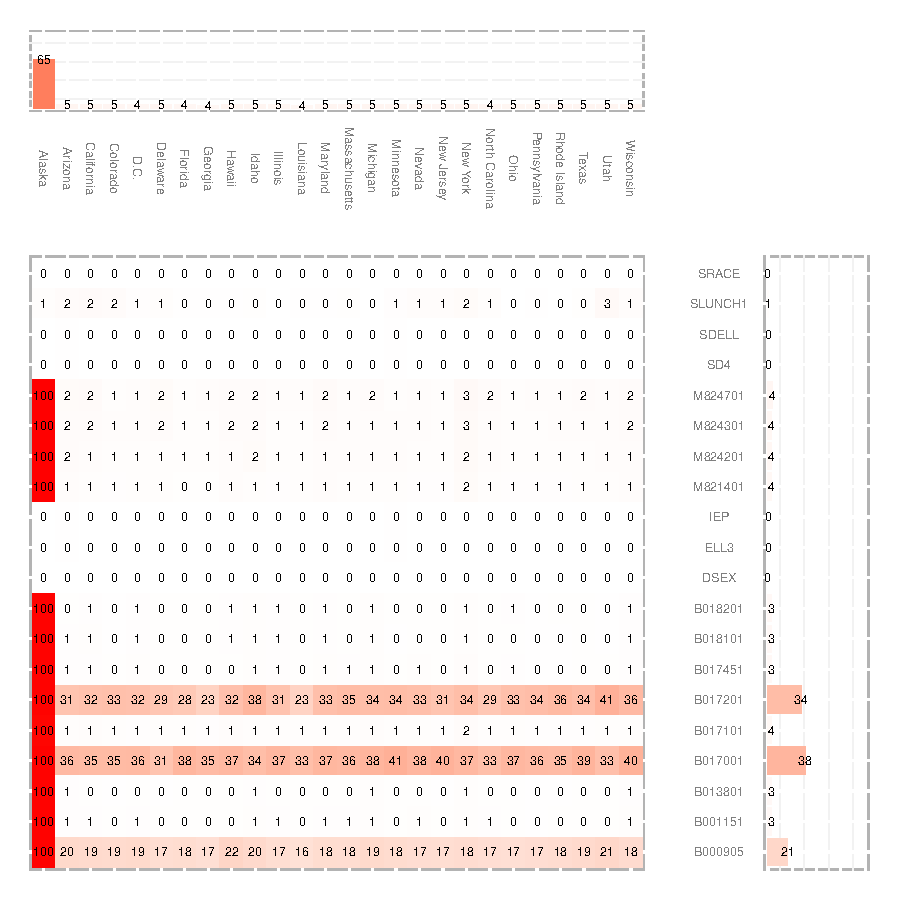
\includegraphics[width=\textwidth]{../Figures2009/g4math-missing.pdf}
\caption{Covariate Missingness for Grade 4 Math}
\label{fig:g4math:missing}
\end{center}
\end{figure}

\begin{figure}[h]
\begin{center}
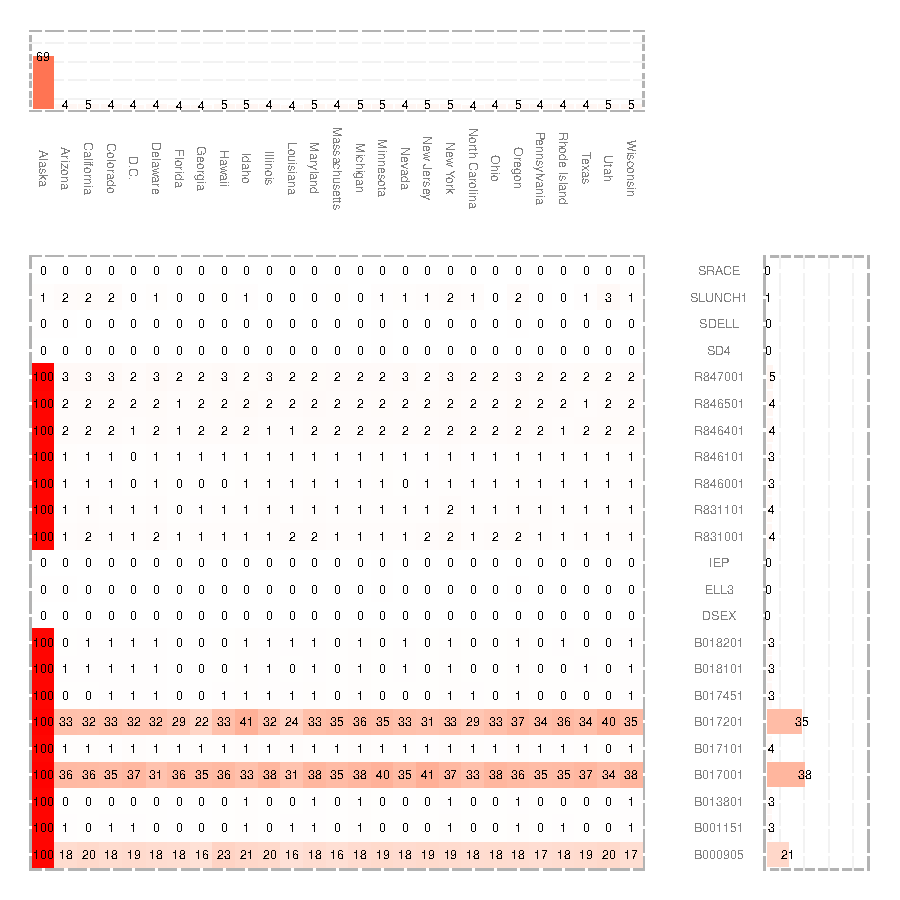
\includegraphics[width=\textwidth]{../Figures2009/g4read-missing.pdf}
\caption{Covariate Missingness for Grade 4 Reading}
\label{fig:g4reading:missing}
\end{center}
\end{figure}

\begin{figure}[h]
\begin{center}
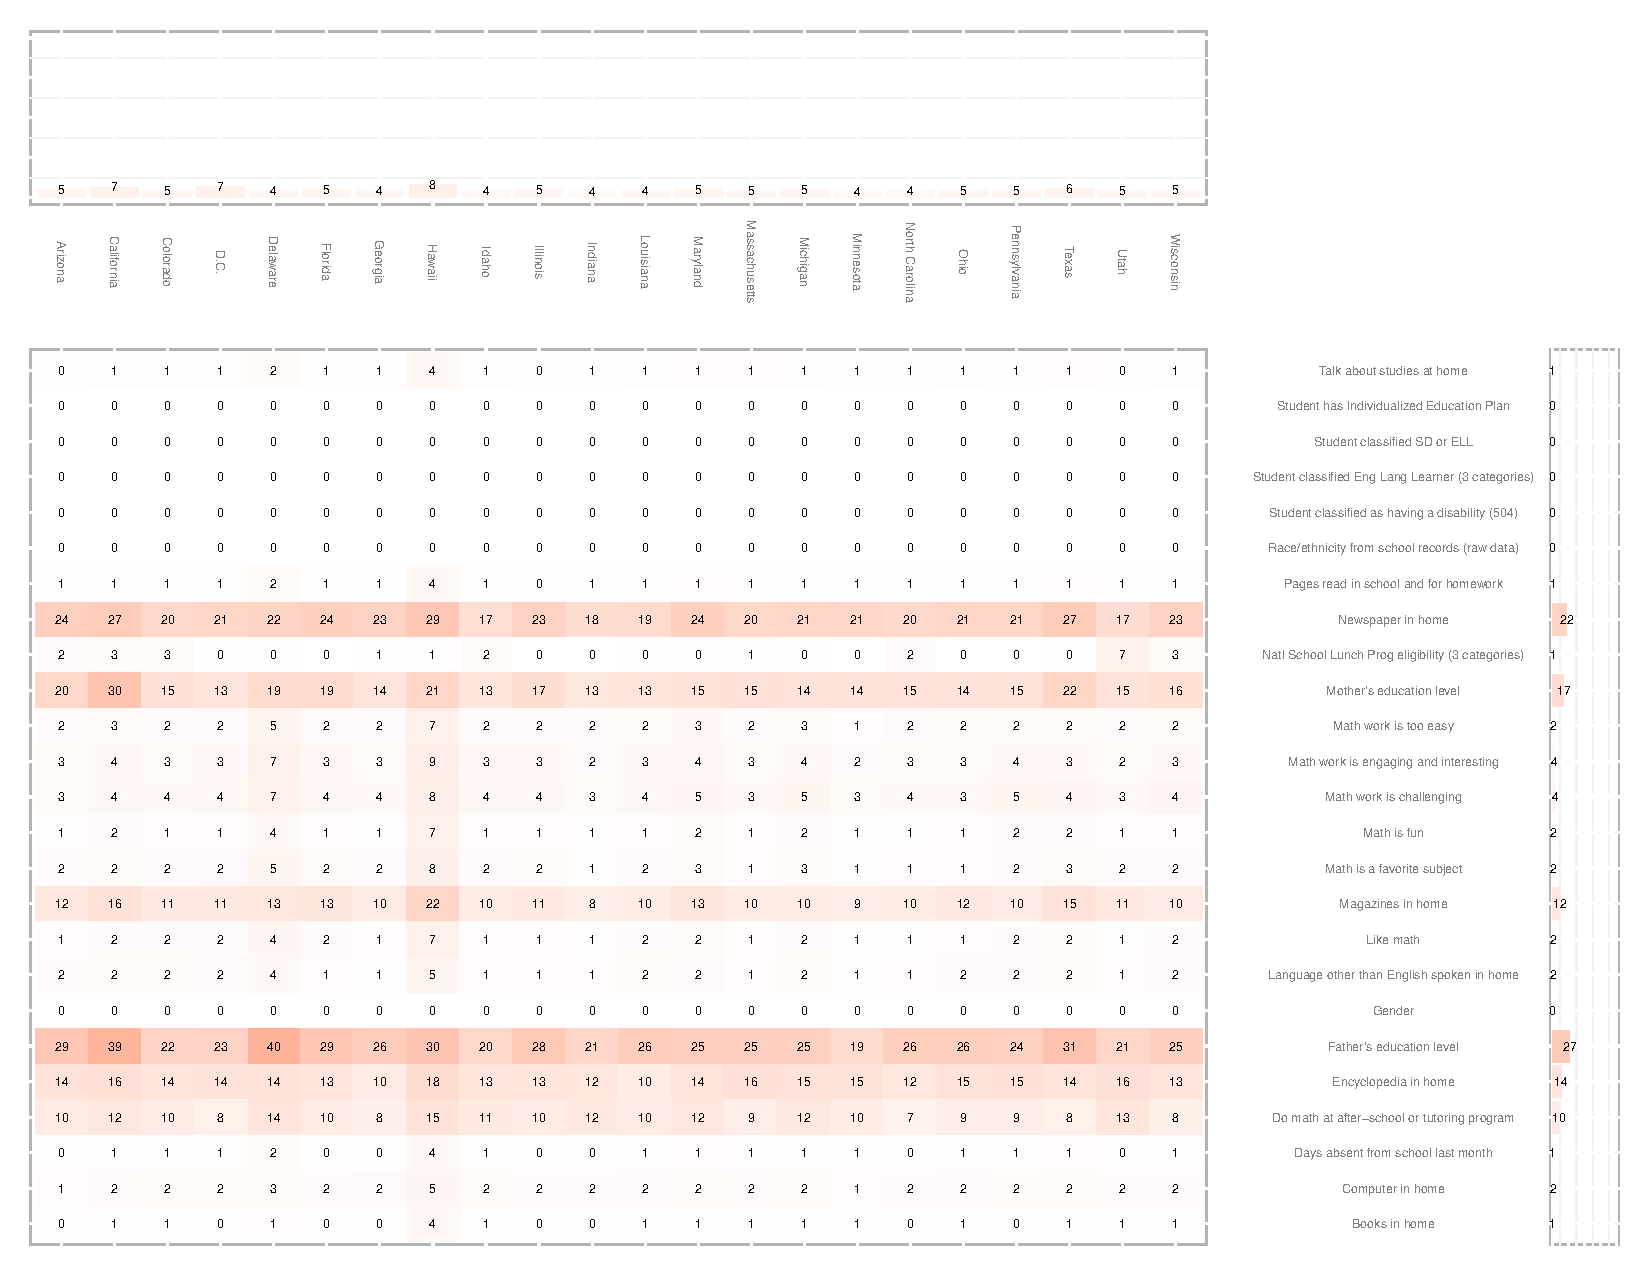
\includegraphics[width=\textwidth]{../Figures2009/g8math-missing.pdf}
\caption{Covariate Missingness for Grade 8 Math}
\label{fig:g8math:missing}
\end{center}
\end{figure}

\begin{figure}[h]
\begin{center}
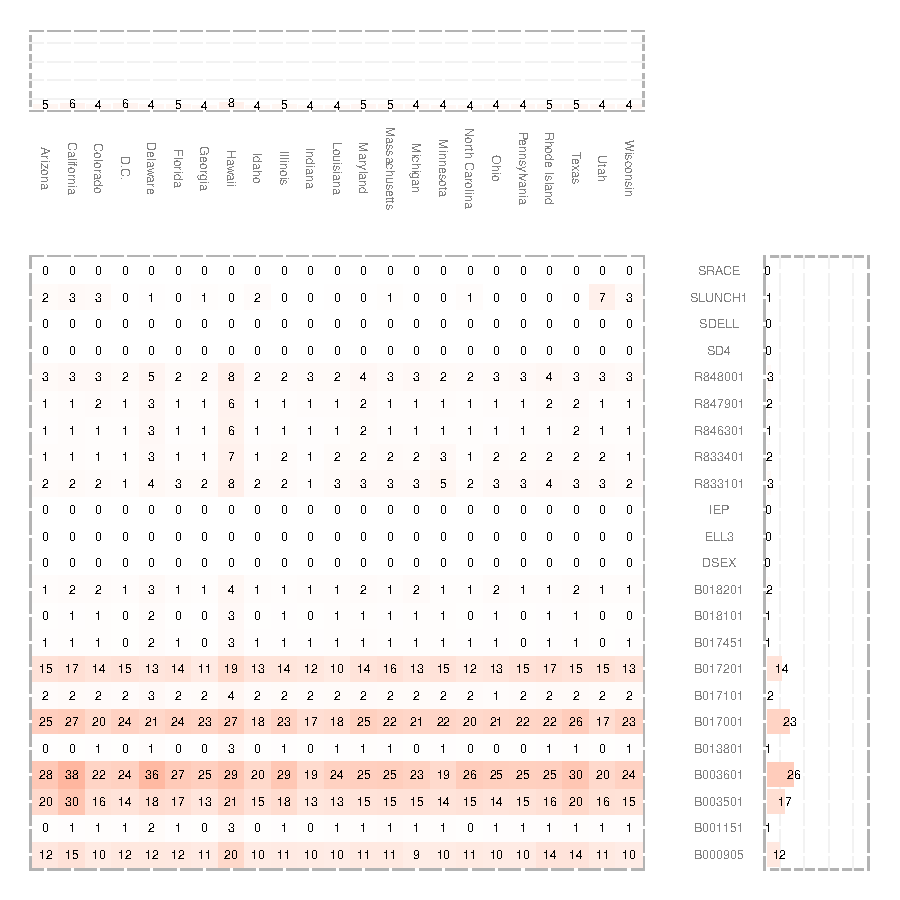
\includegraphics[width=\textwidth]{../Figures2009/g8read-missing.pdf}
\caption{Covariate Missingness for Grade 8 Reading}
\label{fig:g8reading:missing}
\end{center}
\end{figure}


%==================== Appendix F ====================================================================
\clearpage
\addcontentsline{toc}{subsection}{Appendix F: Logistic Regression Full Model Results}
\subsection*{Appendix F\\Logistic Regression Full Model}
\label{appendixlogistic}
%\begin{singlespace}
%% latex table generated in R 2.13.0 by xtable 1.5-6 package
% Sun Jun 26 16:53:32 2011
\begin{longtable}{lrrr@{\extracolsep{10pt}}rrrr}
\caption{Logistic Regression Level 1 Summary: Grade 4 math} \\ 
  \hline
  & \multicolumn{3}{c}{Charter Schools} & \multicolumn{3}{c}{Public Schools} & \\ \cline{2-4} \cline{5-7} State & n & Score & SE & n & Score & SE & Diff \\ \endfirsthead \multicolumn{8}{l}{{...continued from previous page}}\\ \hline & \multicolumn{3}{c}{Charter Schools} & \multicolumn{3}{c}{Public Schools} & \\ \cline{2-4} \cline{5-7} State & n & Score & SE & n & Score & SE & Diff \\ \hline \endhead \hline \endfoot \endlastfoot \hline
Alaska &   7 & 251.69 & 12.92 & 989 & 230.40 & 0.91 & 21.30 \\ 
  Alaska &  11 & 243.73 & 11.19 & 567 & 234.07 & 1.24 & 9.66 \\ 
  Alaska &  78 & 249.08 & 3.07 & 1096 & 251.09 & 0.73 & -2.01 \\ 
  Arizona &  20 & 218.25 & 4.99 & 794 & 224.32 & 1.17 & -6.07 \\ 
  Arizona & 222 & 234.86 & 1.94 & 2381 & 235.32 & 0.60 & -0.46 \\ 
  Arkansas &   4 & 241.24 & 15.43 & 433 & 253.39 & 0.94 & -12.15 \\ 
  Arkansas &   4 & 252.13 & 8.36 & 193 & 253.01 & 1.62 & -0.88 \\ 
  Arkansas &  12 & 245.50 & 5.87 & 133 & 249.91 & 2.13 & -4.41 \\ 
  California &  10 & 221.76 & 9.11 & 827 & 222.99 & 1.22 & -1.23 \\ 
  California & 165 & 227.95 & 2.39 & 6695 & 229.10 & 0.39 & -1.15 \\ 
  California & 101 & 225.82 & 2.69 & 2080 & 222.62 & 0.64 & 3.20 \\ 
  Colorado &  32 & 240.62 & 5.31 & 918 & 228.89 & 0.92 & 11.72 \\ 
  Colorado & 144 & 253.48 & 1.90 & 2150 & 245.43 & 0.58 & 8.05 \\ 
  Connecticut &   6 & 245.19 & 9.24 &  55 & 227.68 & 3.17 & 17.52 \\ 
  Delaware &  40 & 248.90 & 2.78 & 1165 & 248.66 & 0.65 & 0.24 \\ 
  Delaware & 145 & 233.93 & 1.69 & 1727 & 238.87 & 0.56 & -4.93 \\ 
  Dist. of Columbia & 376 & 214.20 & 1.44 & 1555 & 213.74 & 0.81 & 0.46 \\ 
  Florida &   6 & 229.13 & 5.84 & 695 & 226.66 & 0.97 & 2.47 \\ 
  Florida &  45 & 239.46 & 3.04 & 2031 & 239.53 & 0.55 & -0.07 \\ 
  Florida & 165 & 251.07 & 1.54 & 2241 & 248.32 & 0.47 & 2.75 \\ 
  Georgia &  19 & 235.92 & 7.36 & 2349 & 235.12 & 0.58 & 0.80 \\ 
  Georgia &  27 & 229.93 & 4.38 & 1317 & 229.37 & 0.72 & 0.56 \\ 
  Georgia &  35 & 225.07 & 3.38 & 539 & 225.12 & 1.08 & -0.05 \\ 
  Hawaii &   9 & 233.92 & 8.54 & 1254 & 229.08 & 0.82 & 4.84 \\ 
  Hawaii &  15 & 246.91 & 6.30 & 929 & 238.42 & 0.92 & 8.49 \\ 
  Hawaii &  54 & 243.32 & 2.26 & 757 & 247.66 & 0.99 & -4.34 \\ 
  Idaho &  28 & 256.70 & 4.19 & 1130 & 243.43 & 0.70 & 13.27 \\ 
  Idaho &  89 & 258.91 & 2.50 & 1275 & 249.12 & 0.64 & 9.79 \\ 
  Illinois &   6 & 221.80 & 8.61 & 604 & 220.57 & 1.20 & 1.22 \\ 
  Illinois &  24 & 219.03 & 4.76 & 1133 & 219.02 & 0.78 & 0.01 \\ 
  Illinois &  60 & 226.93 & 2.27 & 891 & 214.41 & 0.78 & 12.51 \\ 
  Indiana &   7 & 192.21 & 8.25 &  56 & 220.26 & 3.24 & -28.05 \\ 
  Iowa &   4 & 230.07 & 9.22 &  17 & 240.43 & 6.29 & -10.35 \\ 
  Louisiana &   5 & 247.46 & 10.87 & 589 & 235.04 & 0.96 & 12.41 \\ 
  Louisiana &  18 & 235.47 & 5.20 & 878 & 234.11 & 0.84 & 1.36 \\ 
  Louisiana & 134 & 236.57 & 2.27 & 1382 & 225.71 & 0.68 & 10.85 \\ 
  Maryland &   4 & 215.36 & 5.68 & 678 & 234.03 & 1.05 & -18.67 \\ 
  Maryland &   8 & 215.15 & 5.48 & 336 & 226.60 & 1.49 & -11.45 \\ 
  Maryland &   9 & 212.58 & 8.93 & 151 & 223.72 & 2.13 & -11.15 \\ 
  Massachusetts &   7 & 246.67 & 11.07 & 1325 & 247.03 & 0.73 & -0.37 \\ 
  Massachusetts &  10 & 225.57 & 7.55 & 392 & 235.81 & 1.29 & -10.24 \\ 
  Massachusetts &  39 & 231.15 & 2.64 & 392 & 234.89 & 1.05 & -3.75 \\ 
  Michigan &  14 & 249.97 & 7.42 & 520 & 248.99 & 1.00 & 0.98 \\ 
  Michigan & 328 & 224.79 & 1.56 & 2420 & 237.49 & 0.57 & -12.70 \\ 
  Minnesota &  11 & 253.55 & 8.34 & 1882 & 249.77 & 0.59 & 3.78 \\ 
  Minnesota &  13 & 250.22 & 7.21 & 482 & 244.53 & 1.25 & 5.69 \\ 
  Minnesota &   9 & 245.57 & 5.31 & 152 & 239.14 & 2.30 & 6.43 \\ 
  Missouri &  26 & 199.23 & 4.90 & 161 & 219.72 & 1.77 & -20.48 \\ 
  Nevada &   9 & 224.35 & 8.06 & 1709 & 230.26 & 0.70 & -5.90 \\ 
  Nevada &  12 & 226.30 & 10.06 & 457 & 234.81 & 1.26 & -8.51 \\ 
  Nevada &   6 & 236.05 & 9.83 & 117 & 230.32 & 2.64 & 5.72 \\ 
  New Jersey &   4 & 234.57 & 9.00 & 348 & 234.79 & 1.32 & -0.22 \\ 
  New Jersey &   7 & 229.02 & 9.25 & 419 & 236.38 & 1.18 & -7.36 \\ 
  New Jersey &  23 & 222.19 & 4.18 & 308 & 236.33 & 1.28 & -14.15 \\ 
  New York &   5 & 232.09 & 7.25 & 266 & 230.84 & 1.46 & 1.25 \\ 
  New York &  11 & 232.49 & 5.37 & 142 & 231.51 & 1.87 & 0.98 \\ 
  North Carolina &  13 & 245.21 & 7.59 & 1626 & 240.31 & 0.64 & 4.90 \\ 
  North Carolina &  14 & 256.95 & 6.68 & 965 & 255.17 & 0.77 & 1.78 \\ 
  North Carolina &  49 & 261.52 & 2.78 & 594 & 253.26 & 0.86 & 8.26 \\ 
  Ohio &  14 & 240.94 & 5.13 & 1636 & 250.50 & 0.58 & -9.56 \\ 
  Ohio &  27 & 232.63 & 4.05 & 1012 & 237.13 & 0.80 & -4.50 \\ 
  Ohio &  81 & 217.31 & 2.33 & 1011 & 217.09 & 0.81 & 0.22 \\ 
  Oregon &   7 & 228.47 & 13.59 &  54 & 230.51 & 3.66 & -2.05 \\ 
  Pennsylvania &   4 & 228.45 & 6.72 & 623 & 239.89 & 1.08 & -11.43 \\ 
  Pennsylvania &  48 & 245.15 & 4.33 & 1681 & 247.83 & 0.67 & -2.69 \\ 
  Pennsylvania &  46 & 245.44 & 4.45 & 840 & 242.79 & 0.97 & 2.65 \\ 
  Rhode Island &   9 & 243.08 & 9.24 & 1593 & 241.33 & 0.62 & 1.75 \\ 
  Rhode Island &   4 & 236.79 & 10.48 & 280 & 235.65 & 1.73 & 1.14 \\ 
  Rhode Island &  15 & 220.68 & 5.10 & 129 & 217.75 & 2.98 & 2.94 \\ 
  Tennessee &   4 & 206.64 & 8.92 &  74 & 219.33 & 3.04 & -12.70 \\ 
  Tennessee &   5 & 215.73 & 8.19 &  73 & 216.15 & 3.05 & -0.43 \\ 
  Texas &  19 & 225.34 & 5.12 & 3172 & 239.87 & 0.42 & -14.53 \\ 
  Texas &  37 & 229.58 & 3.86 & 1536 & 235.41 & 0.54 & -5.83 \\ 
  Texas &  70 & 214.56 & 2.47 & 1075 & 226.00 & 0.65 & -11.44 \\ 
  Utah &  12 & 249.95 & 7.67 & 977 & 239.68 & 0.81 & 10.26 \\ 
  Utah &  28 & 254.61 & 4.43 & 1618 & 243.56 & 0.61 & 11.05 \\ 
  Utah &  36 & 245.81 & 4.56 & 530 & 244.48 & 1.09 & 1.33 \\ 
  Wisconsin &  12 & 256.87 & 5.12 & 1952 & 251.29 & 0.53 & 5.58 \\ 
  Wisconsin &   6 & 242.42 & 11.78 & 290 & 235.29 & 1.69 & 7.13 \\ 
  Wisconsin &  38 & 206.92 & 3.54 & 297 & 219.07 & 1.61 & -12.16 \\ 
   \hline
\hline
\label{g4mathlrlevel1}
\end{longtable}
 \clearpage
%% latex table generated in R 2.13.0 by xtable 1.5-6 package
% Sun Jun 26 16:53:32 2011
\begin{table}[ht]
\begin{center}
\caption{Logistic RegressionLevel 2 Summary: Grade 4 math}
\label{g4mathlrlevel2}
\begin{tabular}{lrrrrrr}
  \hline
  State & n & Public & Charter & Diff & \multicolumn{2}{c}{Confidence Interval} \\ \hline
Alaska & 2748 & 240.01 & 248.90 & 8.89 & -2.52 & 20.29 \\ 
  Arizona & 3417 & 232.70 & 230.91 & -1.79 & -7.20 & 3.61 \\ 
  Arkansas & 779 & 252.65 & 244.79 & -7.86 & -20.11 & 4.39 \\ 
  California & 9878 & 227.15 & 226.96 & -0.20 & -6.67 & 6.27 \\ 
  Colorado & 3244 & 240.59 & 249.71 & 9.12 & 3.49 & 14.76 \\ 
  Connecticut &  61 & 227.68 & 245.19 & 17.52 & -2.04 & 37.07 \\ 
  Delaware & 3077 & 242.70 & 239.80 & -2.91 & -6.20 & 0.39 \\ 
  Dist. of Columbia & 1931 & 213.74 & 214.20 & 0.46 & -2.78 & 3.70 \\ 
  Florida & 5183 & 241.87 & 243.45 & 1.58 & -2.90 & 6.07 \\ 
  Georgia & 4286 & 231.98 & 232.59 & 0.61 & -5.48 & 6.70 \\ 
  Hawaii & 3018 & 236.99 & 240.51 & 3.52 & -3.65 & 10.68 \\ 
  Idaho & 2522 & 246.51 & 257.89 & 11.39 & 6.51 & 16.26 \\ 
  Illinois & 2718 & 217.76 & 222.41 & 4.65 & -2.03 & 11.34 \\ 
  Indiana &  63 & 220.26 & 192.21 & -28.05 & -45.77 & -10.33 \\ 
  Iowa &  21 & 240.43 & 230.07 & -10.35 & -33.72 & 13.01 \\ 
  Louisiana & 3006 & 230.06 & 238.39 & 8.33 & 0.26 & 16.40 \\ 
  Maryland & 1186 & 230.49 & 214.93 & -15.56 & -23.57 & -7.55 \\ 
  Massachusetts & 2165 & 242.53 & 239.66 & -2.87 & -11.88 & 6.13 \\ 
  Michigan & 3282 & 239.36 & 228.88 & -10.48 & -18.00 & -2.96 \\ 
  Minnesota & 2549 & 248.08 & 252.40 & 4.32 & -3.87 & 12.51 \\ 
  Missouri & 187 & 219.72 & 199.23 & -20.48 & -30.77 & -10.20 \\ 
  Nevada & 2310 & 231.19 & 225.37 & -5.81 & -16.59 & 4.97 \\ 
  New Jersey & 1109 & 235.86 & 228.74 & -7.12 & -16.11 & 1.87 \\ 
  New York & 424 & 231.08 & 232.23 & 1.15 & -8.02 & 10.32 \\ 
  North Carolina & 3261 & 247.33 & 251.95 & 4.63 & -2.28 & 11.54 \\ 
  Ohio & 3781 & 237.18 & 231.83 & -5.34 & -9.95 & -0.74 \\ 
  Oregon &  61 & 230.51 & 228.47 & -2.05 & -30.21 & 26.11 \\ 
  Pennsylvania & 3242 & 244.92 & 242.00 & -2.92 & -8.99 & 3.15 \\ 
  Rhode Island & 2030 & 238.86 & 240.61 & 1.75 & -8.24 & 11.74 \\ 
  Tennessee & 156 & 217.74 & 211.18 & -6.56 & -19.26 & 6.13 \\ 
  Texas & 5909 & 235.99 & 224.38 & -11.61 & -16.14 & -7.08 \\ 
  Utah & 3201 & 242.53 & 251.61 & 9.09 & 2.51 & 15.67 \\ 
  Wisconsin & 2595 & 245.31 & 248.77 & 3.47 & -5.38 & 12.31 \\ 
   \hline
\end{tabular}
\end{center}
\end{table}
 \clearpage
%% latex table generated in R 2.13.0 by xtable 1.5-6 package
% Sun Jun 26 16:58:36 2011
\begin{longtable}{lrrr@{\extracolsep{10pt}}rrrr}
\caption{Logistic Regression Level 1 Summary: Grade 4 reading} \\ 
  \hline
  & \multicolumn{3}{c}{Charter Schools} & \multicolumn{3}{c}{Public Schools} & \\ \cline{2-4} \cline{5-7} State & n & Score & SE & n & Score & SE & Diff \\ \endfirsthead \multicolumn{8}{l}{{...continued from previous page}}\\ \hline & \multicolumn{3}{c}{Charter Schools} & \multicolumn{3}{c}{Public Schools} & \\ \cline{2-4} \cline{5-7} State & n & Score & SE & n & Score & SE & Diff \\ \hline \endhead \hline \endfoot \endlastfoot \hline
Alaska &   6 & 211.91 & 17.00 & 669 & 204.26 & 1.34 & 7.66 \\ 
  Alaska &   9 & 215.07 & 12.58 & 581 & 219.01 & 1.25 & -3.94 \\ 
  Alaska &  75 & 236.33 & 3.52 & 1062 & 232.96 & 0.83 & 3.36 \\ 
  Arizona &  24 & 197.42 & 7.39 & 691 & 190.95 & 1.68 & 6.47 \\ 
  Arizona & 204 & 207.49 & 2.20 & 2467 & 215.74 & 0.70 & -8.24 \\ 
  Arkansas &  10 & 212.34 & 7.37 &  76 & 236.55 & 3.05 & -24.22 \\ 
  California &  11 & 217.22 & 12.35 & 1248 & 213.28 & 0.91 & 3.94 \\ 
  California & 141 & 207.05 & 3.64 & 5921 & 206.24 & 0.49 & 0.81 \\ 
  California & 113 & 198.92 & 3.20 & 2173 & 194.42 & 0.80 & 4.50 \\ 
  Colorado &  29 & 230.36 & 4.50 & 734 & 216.34 & 1.10 & 14.01 \\ 
  Colorado & 136 & 239.45 & 2.43 & 1865 & 233.00 & 0.69 & 6.45 \\ 
  Connecticut &   8 & 208.95 & 13.12 &  24 & 198.60 & 6.64 & 10.35 \\ 
  Delaware &   4 & 207.83 & 11.91 & 153 & 215.73 & 2.12 & -7.90 \\ 
  Delaware &  32 & 225.70 & 4.13 & 1046 & 232.45 & 0.75 & -6.75 \\ 
  Delaware & 144 & 211.25 & 2.18 & 1629 & 221.79 & 0.68 & -10.54 \\ 
  Dist. of Columbia & 362 & 194.70 & 1.73 & 1405 & 197.49 & 0.98 & -2.79 \\ 
  Florida &   9 & 209.58 & 10.86 & 991 & 208.43 & 1.00 & 1.14 \\ 
  Florida &  42 & 223.47 & 5.38 & 1787 & 225.73 & 0.72 & -2.26 \\ 
  Florida & 146 & 235.45 & 2.17 & 1841 & 230.69 & 0.61 & 4.76 \\ 
  Georgia &  16 & 230.82 & 8.80 & 2273 & 219.94 & 0.66 & 10.88 \\ 
  Georgia &  27 & 203.74 & 5.18 & 1203 & 208.40 & 0.86 & -4.66 \\ 
  Georgia &  38 & 224.64 & 3.99 & 627 & 210.49 & 1.14 & 14.14 \\ 
  Hawaii &  11 & 225.15 & 10.33 & 1434 & 206.68 & 0.87 & 18.47 \\ 
  Hawaii &  23 & 244.08 & 5.32 & 1100 & 218.20 & 1.04 & 25.88 \\ 
  Hawaii &  41 & 236.67 & 4.52 & 566 & 223.94 & 1.44 & 12.73 \\ 
  Idaho &   8 & 236.08 & 10.99 & 796 & 213.81 & 1.09 & 22.27 \\ 
  Idaho &  22 & 235.49 & 5.40 & 1076 & 225.73 & 0.86 & 9.77 \\ 
  Idaho &  83 & 240.83 & 3.10 & 1151 & 236.38 & 0.76 & 4.45 \\ 
  Illinois &   9 & 190.18 & 11.49 & 1117 & 208.34 & 1.09 & -18.15 \\ 
  Illinois &  20 & 202.58 & 5.54 & 814 & 201.39 & 1.16 & 1.19 \\ 
  Illinois &  70 & 200.47 & 3.66 & 938 & 199.48 & 1.00 & 0.98 \\ 
  Indiana &   6 & 177.07 & 11.35 &  35 & 198.62 & 4.43 & -21.55 \\ 
  Louisiana &   4 & 248.42 & 13.60 & 492 & 213.08 & 1.41 & 35.34 \\ 
  Louisiana &  19 & 230.81 & 8.92 & 996 & 213.56 & 1.07 & 17.25 \\ 
  Louisiana & 135 & 216.61 & 3.06 & 1348 & 201.64 & 0.90 & 14.97 \\ 
  Maryland &   4 & 195.92 & 12.26 & 198 & 206.70 & 2.40 & -10.78 \\ 
  Maryland &  11 & 193.14 & 9.27 & 113 & 204.20 & 2.94 & -11.06 \\ 
  Massachusetts &   5 & 200.33 & 14.67 & 813 & 220.62 & 1.21 & -20.29 \\ 
  Massachusetts &  13 & 213.37 & 9.48 & 460 & 206.55 & 1.46 & 6.82 \\ 
  Massachusetts &  42 & 210.66 & 3.97 & 488 & 211.53 & 1.22 & -0.88 \\ 
  Michigan &  16 & 221.85 & 7.89 & 452 & 229.02 & 1.47 & -7.17 \\ 
  Michigan & 317 & 205.34 & 1.98 & 2480 & 221.49 & 0.66 & -16.15 \\ 
  Minnesota &   5 & 221.95 & 12.20 & 1326 & 227.59 & 0.82 & -5.65 \\ 
  Minnesota &  15 & 218.25 & 7.68 & 594 & 223.00 & 1.29 & -4.75 \\ 
  Minnesota &  14 & 209.19 & 11.66 & 189 & 211.19 & 2.47 & -2.00 \\ 
  Missouri &  24 & 184.28 & 7.13 & 222 & 204.53 & 2.03 & -20.25 \\ 
  Nevada &  11 & 196.67 & 17.83 & 1689 & 213.78 & 0.88 & -17.11 \\ 
  Nevada &   5 & 235.20 & 11.36 & 344 & 214.72 & 1.82 & 20.48 \\ 
  Nevada &   6 & 205.52 & 13.08 &  79 & 212.85 & 4.20 & -7.33 \\ 
  New Jersey &   4 & 210.22 & 21.43 & 510 & 223.91 & 1.47 & -13.69 \\ 
  New Jersey &   8 & 218.06 & 8.86 & 352 & 217.21 & 1.58 & 0.86 \\ 
  New Jersey &  24 & 205.80 & 5.96 & 267 & 212.46 & 1.76 & -6.66 \\ 
  New York &  18 & 205.41 & 6.95 & 233 & 206.24 & 1.83 & -0.83 \\ 
  North Carolina &  12 & 221.78 & 9.34 & 1976 & 213.55 & 0.72 & 8.23 \\ 
  North Carolina &  30 & 243.72 & 5.56 & 1344 & 234.89 & 0.80 & 8.83 \\ 
  North Carolina &  40 & 240.38 & 3.97 & 605 & 229.58 & 1.27 & 10.79 \\ 
  Ohio &  12 & 237.76 & 9.23 & 1364 & 231.20 & 0.74 & 6.56 \\ 
  Ohio &  27 & 208.98 & 6.27 & 1280 & 219.92 & 0.85 & -10.93 \\ 
  Ohio &  69 & 205.92 & 3.32 & 923 & 200.65 & 0.99 & 5.27 \\ 
  Oregon &   7 & 237.49 & 4.44 & 1146 & 228.47 & 0.79 & 9.02 \\ 
  Oregon &   5 & 224.19 & 13.11 &  47 & 222.73 & 4.35 & 1.46 \\ 
  Pennsylvania &   5 & 187.37 & 14.07 & 629 & 214.15 & 1.31 & -26.77 \\ 
  Pennsylvania &  35 & 228.54 & 5.57 & 1531 & 229.87 & 0.87 & -1.33 \\ 
  Pennsylvania &  66 & 226.47 & 3.42 & 1088 & 231.98 & 1.05 & -5.51 \\ 
  Rhode Island &  11 & 223.91 & 9.42 & 1485 & 223.74 & 0.85 & 0.18 \\ 
  Rhode Island &  14 & 224.80 & 7.08 & 109 & 194.22 & 3.64 & 30.58 \\ 
  South Carolina &   4 & 151.84 & 13.52 &  31 & 212.34 & 5.09 & -60.51 \\ 
  Tennessee &   8 & 208.04 & 6.23 &  87 & 196.10 & 3.68 & 11.94 \\ 
  Texas &  18 & 206.90 & 6.99 & 2857 & 225.56 & 0.59 & -18.66 \\ 
  Texas &  37 & 201.71 & 4.68 & 1922 & 211.31 & 0.61 & -9.60 \\ 
  Texas &  55 & 193.32 & 3.96 & 905 & 202.74 & 0.88 & -9.43 \\ 
  Utah &   7 & 220.76 & 10.13 & 879 & 221.48 & 0.98 & -0.72 \\ 
  Utah &  35 & 225.00 & 4.87 & 1649 & 230.03 & 0.72 & -5.03 \\ 
  Utah &  27 & 213.96 & 8.76 & 446 & 218.44 & 1.79 & -4.48 \\ 
  Wisconsin &  12 & 227.79 & 9.99 & 1691 & 227.42 & 0.75 & 0.36 \\ 
  Wisconsin &  43 & 166.48 & 5.68 & 272 & 197.61 & 2.25 & -31.13 \\ 
  Wyoming &   5 & 239.84 & 4.23 &  52 & 238.69 & 3.06 & 1.15 \\ 
   \hline
\hline
\label{g4readinglrlevel1}
\end{longtable}
 \clearpage
%% latex table generated in R 2.13.0 by xtable 1.5-6 package
% Sun Jun 26 16:58:36 2011
\begin{table}[ht]
\begin{center}
\caption{Logistic RegressionLevel 2 Summary: Grade 4 reading}
\label{g4readinglrlevel2}
\begin{tabular}{lrrrrrr}
  \hline
  State & n & Public & Charter & Diff & \multicolumn{2}{c}{Confidence Interval} \\ \hline
Alaska & 2402 & 221.47 & 224.24 & 2.77 & -11.30 & 16.85 \\ 
  Arizona & 3386 & 210.50 & 205.37 & -5.14 & -12.90 & 2.63 \\ 
  Arkansas &  86 & 236.55 & 212.34 & -24.22 & -40.08 & -8.35 \\ 
  California & 9607 & 204.35 & 206.45 & 2.10 & -6.61 & 10.81 \\ 
  Colorado & 2764 & 228.40 & 236.94 & 8.54 & 3.36 & 13.71 \\ 
  Connecticut &  32 & 198.60 & 208.95 & 10.35 & -19.68 & 40.38 \\ 
  Delaware & 3008 & 225.29 & 216.25 & -9.04 & -17.54 & -0.55 \\ 
  Dist. of Columbia & 1767 & 197.49 & 194.70 & -2.79 & -6.69 & 1.11 \\ 
  Florida & 4816 & 224.19 & 225.53 & 1.34 & -6.75 & 9.44 \\ 
  Georgia & 4184 & 215.05 & 221.87 & 6.83 & -0.41 & 14.06 \\ 
  Hawaii & 3175 & 214.06 & 234.05 & 19.99 & 11.74 & 28.24 \\ 
  Idaho & 3136 & 226.86 & 237.74 & 10.88 & 2.56 & 19.20 \\ 
  Illinois & 2968 & 203.38 & 197.16 & -6.22 & -14.98 & 2.54 \\ 
  Indiana &  41 & 198.62 & 177.07 & -21.55 & -46.20 & 3.10 \\ 
  Louisiana & 2994 & 207.58 & 226.70 & 19.12 & 8.22 & 30.01 \\ 
  Maryland & 326 & 205.75 & 194.86 & -10.89 & -26.46 & 4.69 \\ 
  Massachusetts & 1821 & 214.32 & 206.72 & -7.60 & -19.40 & 4.21 \\ 
  Michigan & 3265 & 222.57 & 207.71 & -14.86 & -22.99 & -6.73 \\ 
  Minnesota & 2143 & 224.73 & 219.69 & -5.05 & -17.31 & 7.22 \\ 
  Missouri & 246 & 204.53 & 184.28 & -20.25 & -34.85 & -5.64 \\ 
  Nevada & 2134 & 213.90 & 203.32 & -10.58 & -27.11 & 5.96 \\ 
  New Jersey & 1165 & 218.98 & 211.54 & -7.44 & -23.20 & 8.32 \\ 
  New York & 251 & 206.24 & 205.41 & -0.83 & -14.98 & 13.32 \\ 
  North Carolina & 4007 & 223.45 & 232.30 & 8.85 & 1.21 & 16.49 \\ 
  Ohio & 3675 & 218.94 & 218.93 & -0.01 & -7.68 & 7.66 \\ 
  Oregon & 1205 & 228.22 & 236.92 & 8.69 & -5.56 & 22.95 \\ 
  Pennsylvania & 3354 & 227.62 & 220.04 & -7.58 & -17.79 & 2.64 \\ 
  Rhode Island & 1619 & 221.50 & 223.98 & 2.49 & -9.64 & 14.62 \\ 
  South Carolina &  35 & 212.34 & 151.84 & -60.51 & -89.89 & -31.12 \\ 
  Tennessee &  95 & 196.10 & 208.04 & 11.94 & -2.43 & 26.30 \\ 
  Texas & 5794 & 216.96 & 202.89 & -14.07 & -20.20 & -7.94 \\ 
  Utah & 3043 & 225.74 & 222.05 & -3.69 & -13.11 & 5.74 \\ 
  Wisconsin & 2018 & 222.77 & 218.22 & -4.55 & -16.06 & 6.95 \\ 
  Wyoming &  57 & 238.69 & 239.84 & 1.15 & -9.31 & 11.61 \\ 
   \hline
\end{tabular}
\end{center}
\end{table}
 \clearpage
%% latex table generated in R 2.13.0 by xtable 1.5-6 package
% Sun Jun 26 17:04:11 2011
\begin{longtable}{lrrr@{\extracolsep{10pt}}rrrr}
\caption{Logistic Regression Level 1 Summary: Grade 8 math} \\ 
  \hline
  & \multicolumn{3}{c}{Charter Schools} & \multicolumn{3}{c}{Public Schools} & \\ \cline{2-4} \cline{5-7} State & n & Score & SE & n & Score & SE & Diff \\ \endfirsthead \multicolumn{8}{l}{{...continued from previous page}}\\ \hline & \multicolumn{3}{c}{Charter Schools} & \multicolumn{3}{c}{Public Schools} & \\ \cline{2-4} \cline{5-7} State & n & Score & SE & n & Score & SE & Diff \\ \hline \endhead \hline \endfoot \endlastfoot \hline
Alaska &   8 & 282.23 & 13.07 & 566 & 289.08 & 1.28 & -6.86 \\ 
  Alaska &  28 & 296.83 & 5.08 & 866 & 288.67 & 1.02 & 8.17 \\ 
  Alaska &  31 & 285.36 & 6.01 & 514 & 291.30 & 1.39 & -5.94 \\ 
  Arizona &   4 & 251.17 & 11.93 & 367 & 258.42 & 1.94 & -7.25 \\ 
  Arizona &   5 & 274.55 & 13.15 & 529 & 274.79 & 1.47 & -0.24 \\ 
  Arizona &  19 & 267.67 & 8.45 & 576 & 278.21 & 1.28 & -10.54 \\ 
  Arizona &  65 & 285.50 & 4.55 & 786 & 285.32 & 1.15 & 0.18 \\ 
  Arkansas &   7 & 278.36 & 13.96 & 563 & 280.66 & 1.44 & -2.31 \\ 
  Arkansas &   9 & 260.44 & 13.27 & 227 & 267.74 & 2.14 & -7.30 \\ 
  Arkansas &  10 & 263.32 & 15.01 & 126 & 266.82 & 2.59 & -3.50 \\ 
  California &   5 & 260.31 & 27.55 & 440 & 263.49 & 1.73 & -3.18 \\ 
  California &  91 & 274.37 & 4.25 & 2923 & 267.84 & 0.71 & 6.52 \\ 
  California & 247 & 276.20 & 2.34 & 3352 & 269.03 & 0.66 & 7.17 \\ 
  Colorado &   4 & 268.11 & 17.25 & 365 & 279.31 & 1.61 & -11.20 \\ 
  Colorado &  16 & 273.96 & 10.09 & 534 & 292.45 & 1.36 & -18.49 \\ 
  Colorado &  87 & 307.28 & 3.55 & 971 & 298.61 & 1.03 & 8.67 \\ 
  Delaware &  25 & 271.91 & 7.73 & 634 & 277.43 & 1.23 & -5.51 \\ 
  Delaware & 144 & 294.44 & 2.81 & 1707 & 286.23 & 0.73 & 8.21 \\ 
  Dist. of Columbia & 572 & 257.81 & 1.21 & 1135 & 241.65 & 0.98 & 16.16 \\ 
  Florida &  15 & 265.68 & 9.18 & 681 & 264.59 & 1.23 & 1.09 \\ 
  Florida &  36 & 273.70 & 4.83 & 1560 & 279.52 & 0.84 & -5.82 \\ 
  Florida & 117 & 277.58 & 2.95 & 1332 & 283.70 & 0.90 & -6.12 \\ 
  Georgia &   5 & 250.76 & 12.52 & 1188 & 282.04 & 0.93 & -31.29 \\ 
  Georgia &   8 & 251.32 & 9.63 & 889 & 266.68 & 1.11 & -15.36 \\ 
  Georgia &  25 & 268.60 & 6.30 & 820 & 260.04 & 1.06 & 8.56 \\ 
  Georgia &  26 & 278.36 & 8.87 & 377 & 266.51 & 1.56 & 11.84 \\ 
  Hawaii &  34 & 264.33 & 6.08 & 838 & 267.44 & 1.24 & -3.11 \\ 
  Hawaii &  95 & 267.73 & 3.67 & 1092 & 272.05 & 1.05 & -4.32 \\ 
  Idaho &   9 & 292.08 & 9.27 & 883 & 285.35 & 1.01 & 6.73 \\ 
  Idaho &  20 & 293.78 & 6.64 & 586 & 291.75 & 1.27 & 2.03 \\ 
  Idaho &  27 & 308.47 & 5.26 & 350 & 295.02 & 1.66 & 13.45 \\ 
  Illinois &   9 & 296.70 & 11.27 & 2370 & 275.28 & 0.75 & 21.42 \\ 
  Illinois &   6 & 286.57 & 13.01 & 837 & 271.99 & 1.20 & 14.59 \\ 
  Illinois &   5 & 292.64 & 12.22 & 308 & 266.56 & 1.71 & 26.08 \\ 
  Illinois &  13 & 262.10 & 7.01 & 126 & 261.99 & 2.56 & 0.11 \\ 
  Indiana &  10 & 228.33 & 6.73 &  65 & 259.22 & 3.60 & -30.89 \\ 
  Kansas &   7 & 298.62 & 13.04 & 399 & 294.59 & 1.40 & 4.03 \\ 
  Kansas &   6 & 288.01 & 14.73 &  71 & 289.80 & 3.10 & -1.79 \\ 
  Louisiana &  10 & 280.07 & 9.40 & 616 & 277.27 & 1.08 & 2.80 \\ 
  Louisiana &  15 & 271.46 & 10.16 & 628 & 274.75 & 1.17 & -3.29 \\ 
  Louisiana &  69 & 281.48 & 4.19 & 658 & 265.98 & 1.08 & 15.50 \\ 
  Maryland &   5 & 299.46 & 20.83 &  33 & 300.83 & 4.84 & -1.37 \\ 
  Massachusetts &   4 & 262.25 & 10.11 & 990 & 286.08 & 1.09 & -23.83 \\ 
  Massachusetts &  12 & 298.35 & 11.54 & 1159 & 298.46 & 0.98 & -0.11 \\ 
  Massachusetts &  18 & 301.00 & 8.97 & 696 & 297.72 & 1.25 & 3.28 \\ 
  Massachusetts &  20 & 291.97 & 7.48 & 259 & 292.84 & 2.12 & -0.86 \\ 
  Michigan &   8 & 261.74 & 17.09 & 576 & 279.93 & 1.36 & -18.20 \\ 
  Michigan &  30 & 273.00 & 6.87 & 1083 & 287.00 & 0.97 & -14.00 \\ 
  Michigan &  89 & 252.66 & 3.38 & 653 & 261.93 & 1.47 & -9.26 \\ 
  Minnesota &  13 & 278.28 & 7.76 &  84 & 278.70 & 4.24 & -0.42 \\ 
  Missouri &  30 & 236.28 & 3.73 & 240 & 251.91 & 1.57 & -15.63 \\ 
  New Mexico &   8 & 272.01 & 14.07 & 823 & 272.40 & 1.05 & -0.39 \\ 
  New Mexico &  24 & 278.42 & 6.07 & 570 & 273.49 & 1.22 & 4.93 \\ 
  New Mexico &  21 & 267.86 & 6.76 & 242 & 267.02 & 1.99 & 0.85 \\ 
  New York &   8 & 210.66 & 11.05 &  81 & 242.12 & 3.53 & -31.46 \\ 
  North Carolina &  22 & 276.52 & 7.49 & 1905 & 283.78 & 0.77 & -7.26 \\ 
  North Carolina &  25 & 291.37 & 6.72 & 935 & 286.40 & 1.18 & 4.96 \\ 
  North Carolina &  21 & 272.50 & 9.56 & 271 & 280.81 & 2.30 & -8.31 \\ 
  Ohio &   8 & 261.88 & 6.93 & 455 & 262.69 & 1.36 & -0.81 \\ 
  Ohio &   9 & 267.06 & 6.37 & 382 & 254.88 & 1.55 & 12.18 \\ 
  Ohio &  25 & 242.80 & 5.29 & 282 & 250.11 & 1.69 & -7.31 \\ 
  Oregon &   6 & 278.27 & 14.50 & 702 & 290.36 & 1.20 & -12.09 \\ 
  Oregon &  16 & 281.27 & 7.72 & 391 & 295.69 & 1.73 & -14.41 \\ 
  Oregon &  18 & 308.87 & 6.60 & 208 & 289.15 & 2.30 & 19.72 \\ 
  Pennsylvania &   7 & 287.97 & 9.58 & 1130 & 294.47 & 0.89 & -6.49 \\ 
  Pennsylvania &   5 & 267.26 & 13.32 & 670 & 291.59 & 1.22 & -24.32 \\ 
  Pennsylvania &  49 & 246.05 & 3.59 & 280 & 261.26 & 2.12 & -15.21 \\ 
  Rhode Island &   5 & 290.25 & 14.03 & 333 & 269.54 & 2.06 & 20.71 \\ 
  Rhode Island &   5 & 272.15 & 8.88 & 152 & 253.43 & 2.87 & 18.71 \\ 
  Rhode Island &  17 & 269.32 & 7.39 & 179 & 250.72 & 2.40 & 18.60 \\ 
  South Carolina &   9 & 310.20 & 9.47 &  66 & 297.73 & 4.17 & 12.47 \\ 
  Tennessee &  48 & 262.92 & 3.42 & 306 & 257.16 & 1.53 & 5.77 \\ 
  Texas &  26 & 276.56 & 7.45 & 2392 & 284.31 & 0.70 & -7.75 \\ 
  Texas &  68 & 286.28 & 4.38 & 2265 & 284.36 & 0.64 & 1.92 \\ 
  Texas &  87 & 295.35 & 3.41 & 1046 & 285.49 & 0.91 & 9.86 \\ 
  Utah &   8 & 270.09 & 4.48 & 773 & 290.62 & 1.03 & -20.52 \\ 
  Utah &  13 & 293.26 & 10.29 & 412 & 291.63 & 1.61 & 1.63 \\ 
  Utah &  14 & 281.80 & 12.31 & 175 & 277.36 & 3.00 & 4.44 \\ 
  Wisconsin &  10 & 290.78 & 8.70 & 1132 & 292.81 & 0.90 & -2.03 \\ 
  Wisconsin &  22 & 286.88 & 7.49 & 539 & 287.14 & 1.50 & -0.26 \\ 
  Wisconsin &  66 & 265.71 & 4.03 & 389 & 263.27 & 1.75 & 2.43 \\ 
   \hline
\hline
\label{g8mathlrlevel1}
\end{longtable}
 \clearpage
%% latex table generated in R 2.13.0 by xtable 1.5-6 package
% Sun Jun 26 17:04:11 2011
\begin{table}[ht]
\begin{center}
\caption{Logistic RegressionLevel 2 Summary: Grade 8 math}
\label{g8mathlrlevel2}
\begin{tabular}{lrrrrrr}
  \hline
  State & n & Public & Charter & Diff & \multicolumn{2}{c}{Confidence Interval} \\ \hline
Alaska & 2013 & 289.50 & 289.56 & 0.06 & -10.00 & 10.13 \\ 
  Arizona & 2351 & 276.88 & 273.08 & -3.80 & -13.80 & 6.20 \\ 
  Arkansas & 942 & 275.43 & 271.70 & -3.73 & -19.88 & 12.42 \\ 
  California & 7058 & 268.17 & 274.42 & 6.24 & -12.08 & 24.57 \\ 
  Colorado & 1977 & 293.29 & 290.70 & -2.60 & -15.95 & 10.76 \\ 
  Delaware & 2510 & 283.92 & 288.53 & 4.61 & -3.58 & 12.79 \\ 
  Dist. of Columbia & 1707 & 241.65 & 257.81 & 16.16 & 13.12 & 19.20 \\ 
  Florida & 3741 & 278.36 & 273.71 & -4.65 & -11.79 & 2.49 \\ 
  Georgia & 3338 & 270.47 & 258.76 & -11.71 & -21.19 & -2.24 \\ 
  Hawaii & 2059 & 270.10 & 266.29 & -3.81 & -10.95 & 3.33 \\ 
  Idaho & 1875 & 289.36 & 295.93 & 6.56 & -1.79 & 14.91 \\ 
  Illinois & 3674 & 273.28 & 292.72 & 19.44 & 8.42 & 30.47 \\ 
  Indiana &  75 & 259.22 & 228.33 & -30.89 & -46.10 & -15.69 \\ 
  Kansas & 483 & 293.82 & 296.92 & 3.10 & -16.52 & 22.72 \\ 
  Louisiana & 1996 & 272.34 & 277.81 & 5.47 & -4.07 & 15.00 \\ 
  Maryland &  38 & 300.83 & 299.46 & -1.37 & -44.74 & 42.00 \\ 
  Massachusetts & 3158 & 293.90 & 287.02 & -6.87 & -16.43 & 2.68 \\ 
  Michigan & 2439 & 277.68 & 264.12 & -13.56 & -25.89 & -1.24 \\ 
  Minnesota &  97 & 278.70 & 278.28 & -0.42 & -17.97 & 17.13 \\ 
  Missouri & 270 & 251.91 & 236.28 & -15.63 & -23.58 & -7.67 \\ 
  New Mexico & 1688 & 271.94 & 273.62 & 1.68 & -9.40 & 12.75 \\ 
  New York &  89 & 242.12 & 210.66 & -31.46 & -54.51 & -8.40 \\ 
  North Carolina & 3179 & 284.30 & 280.63 & -3.67 & -12.91 & 5.57 \\ 
  Ohio & 1161 & 256.73 & 258.58 & 1.85 & -5.43 & 9.12 \\ 
  Oregon & 1341 & 291.77 & 284.34 & -7.43 & -19.19 & 4.32 \\ 
  Pennsylvania & 2141 & 288.46 & 275.00 & -13.45 & -24.56 & -2.35 \\ 
  Rhode Island & 691 & 260.54 & 280.20 & 19.66 & 7.44 & 31.87 \\ 
  South Carolina &  75 & 297.73 & 310.20 & 12.47 & -8.15 & 33.09 \\ 
  Tennessee & 354 & 257.16 & 262.92 & 5.77 & -1.61 & 13.15 \\ 
  Texas & 5884 & 284.55 & 284.03 & -0.53 & -6.66 & 5.61 \\ 
  Utah & 1395 & 289.13 & 278.74 & -10.39 & -21.53 & 0.75 \\ 
  Wisconsin & 2158 & 285.11 & 284.48 & -0.63 & -8.75 & 7.49 \\ 
   \hline
\end{tabular}
\end{center}
\end{table}
 \clearpage
%% latex table generated in R 2.13.0 by xtable 1.5-6 package
% Sun Jun 26 17:09:25 2011
\begin{longtable}{lrrr@{\extracolsep{10pt}}rrrr}
\caption{Logistic Regression Level 1 Summary: Grade 8 reading} \\ 
  \hline
  & \multicolumn{3}{c}{Charter Schools} & \multicolumn{3}{c}{Public Schools} & \\ \cline{2-4} \cline{5-7} State & n & Score & SE & n & Score & SE & Diff \\ \endfirsthead \multicolumn{8}{l}{{...continued from previous page}}\\ \hline & \multicolumn{3}{c}{Charter Schools} & \multicolumn{3}{c}{Public Schools} & \\ \cline{2-4} \cline{5-7} State & n & Score & SE & n & Score & SE & Diff \\ \hline \endhead \hline \endfoot \endlastfoot \hline
Alaska &   8 & 258.76 & 11.10 & 738 & 260.30 & 1.16 & -1.53 \\ 
  Alaska &  29 & 265.06 & 4.34 & 843 & 264.70 & 1.02 & 0.36 \\ 
  Alaska &  34 & 275.81 & 4.82 & 524 & 262.60 & 1.37 & 13.20 \\ 
  Arizona &   6 & 228.21 & 11.03 & 567 & 243.42 & 1.33 & -15.21 \\ 
  Arizona &  17 & 238.54 & 9.40 & 795 & 254.43 & 1.22 & -15.89 \\ 
  Arizona &  82 & 267.59 & 3.53 & 950 & 265.91 & 1.00 & 1.68 \\ 
  Arkansas &   5 & 276.15 & 15.75 & 1503 & 261.69 & 0.78 & 14.46 \\ 
  Arkansas &   5 & 260.25 & 13.11 & 515 & 255.26 & 1.36 & 5.00 \\ 
  Arkansas &   7 & 246.50 & 10.73 & 217 & 245.83 & 2.33 & 0.67 \\ 
  Arkansas &  14 & 248.94 & 7.92 & 144 & 243.10 & 2.82 & 5.84 \\ 
  California &  95 & 246.86 & 4.37 & 3228 & 247.77 & 0.61 & -0.91 \\ 
  California & 254 & 253.00 & 2.56 & 3633 & 250.05 & 0.64 & 2.95 \\ 
  Colorado &   5 & 279.06 & 15.47 & 501 & 259.46 & 1.15 & 19.59 \\ 
  Colorado &  16 & 279.48 & 5.89 & 642 & 269.84 & 1.00 & 9.65 \\ 
  Colorado &  83 & 288.72 & 2.75 & 874 & 278.84 & 0.84 & 9.87 \\ 
  Delaware &   4 & 255.44 & 14.34 & 203 & 256.61 & 1.87 & -1.17 \\ 
  Delaware &  16 & 267.79 & 5.75 & 627 & 257.64 & 1.12 & 10.15 \\ 
  Delaware & 174 & 277.75 & 2.31 & 1683 & 268.15 & 0.66 & 9.60 \\ 
  Dist. of Columbia & 558 & 250.14 & 1.15 & 1125 & 234.51 & 0.93 & 15.62 \\ 
  Florida &   9 & 254.26 & 14.05 & 618 & 240.65 & 1.40 & 13.60 \\ 
  Florida &  42 & 262.65 & 3.38 & 1383 & 258.18 & 0.83 & 4.47 \\ 
  Florida & 144 & 271.86 & 2.24 & 1720 & 268.34 & 0.70 & 3.53 \\ 
  Georgia &   4 & 257.03 & 7.80 & 956 & 261.02 & 1.03 & -3.99 \\ 
  Georgia &  15 & 256.64 & 10.02 & 1164 & 256.48 & 0.95 & 0.16 \\ 
  Georgia &  15 & 246.95 & 6.44 & 710 & 249.26 & 1.09 & -2.31 \\ 
  Georgia &  29 & 259.81 & 4.73 & 402 & 252.65 & 1.42 & 7.16 \\ 
  Hawaii &   6 & 265.72 & 5.18 & 310 & 247.16 & 1.84 & 18.56 \\ 
  Hawaii &  25 & 255.19 & 6.10 & 1031 & 250.41 & 1.06 & 4.78 \\ 
  Hawaii & 110 & 259.36 & 2.66 & 1306 & 253.83 & 0.90 & 5.53 \\ 
  Idaho &  11 & 281.22 & 4.51 & 970 & 265.65 & 0.79 & 15.56 \\ 
  Idaho &  19 & 278.84 & 5.49 & 825 & 271.04 & 0.88 & 7.80 \\ 
  Idaho &  28 & 291.50 & 6.19 & 371 & 275.61 & 1.39 & 15.89 \\ 
  Illinois &   6 & 275.17 & 15.24 & 2192 & 260.96 & 0.69 & 14.21 \\ 
  Illinois &  11 & 252.37 & 7.90 & 933 & 254.58 & 1.06 & -2.20 \\ 
  Illinois &  11 & 257.48 & 7.44 & 407 & 251.51 & 1.46 & 5.96 \\ 
  Illinois &  14 & 262.89 & 3.86 & 188 & 249.32 & 2.05 & 13.57 \\ 
  Indiana &  11 & 243.69 & 6.88 &  66 & 246.23 & 3.64 & -2.55 \\ 
  Kansas &  11 & 270.13 & 7.80 & 583 & 272.02 & 1.00 & -1.89 \\ 
  Louisiana &   8 & 274.18 & 8.95 & 630 & 255.47 & 1.22 & 18.70 \\ 
  Louisiana &  20 & 254.76 & 6.67 & 673 & 256.99 & 1.11 & -2.24 \\ 
  Louisiana &  72 & 265.19 & 4.00 & 777 & 250.13 & 0.98 & 15.06 \\ 
  Massachusetts &   4 & 274.31 & 19.71 & 848 & 266.87 & 0.99 & 7.44 \\ 
  Massachusetts &  14 & 280.60 & 6.71 & 1462 & 270.44 & 0.77 & 10.16 \\ 
  Massachusetts &  25 & 277.04 & 6.76 & 855 & 272.34 & 1.07 & 4.70 \\ 
  Massachusetts &  14 & 282.61 & 10.82 & 216 & 273.21 & 2.35 & 9.40 \\ 
  Michigan &  18 & 262.75 & 10.06 & 994 & 261.63 & 0.93 & 1.11 \\ 
  Michigan &  20 & 271.51 & 5.38 & 949 & 271.48 & 0.90 & 0.03 \\ 
  Michigan &  93 & 252.18 & 2.55 & 487 & 238.57 & 1.53 & 13.61 \\ 
  Minnesota &  14 & 260.03 & 9.48 &  49 & 256.85 & 4.69 & 3.18 \\ 
  Missouri &  42 & 230.35 & 4.36 & 270 & 243.19 & 1.62 & -12.84 \\ 
  New Mexico &  13 & 250.75 & 5.88 & 983 & 249.78 & 0.98 & 0.97 \\ 
  New Mexico &  21 & 251.70 & 4.92 & 816 & 257.04 & 0.95 & -5.34 \\ 
  New Mexico &  23 & 260.34 & 4.93 & 295 & 256.57 & 1.50 & 3.77 \\ 
  New York &  12 & 212.04 & 6.02 &  55 & 229.16 & 4.50 & -17.12 \\ 
  North Carolina &  21 & 263.29 & 6.78 & 1976 & 257.59 & 0.73 & 5.70 \\ 
  North Carolina &  34 & 258.12 & 7.47 & 1211 & 260.62 & 1.04 & -2.50 \\ 
  North Carolina &  19 & 254.46 & 9.14 & 271 & 253.04 & 2.40 & 1.42 \\ 
  Ohio &   6 & 243.85 & 10.62 & 2272 & 270.60 & 0.59 & -26.74 \\ 
  Ohio &   6 & 228.90 & 8.28 & 513 & 246.61 & 1.20 & -17.71 \\ 
  Ohio &   6 & 257.02 & 10.31 & 338 & 245.86 & 1.41 & 11.16 \\ 
  Ohio &  27 & 241.83 & 7.11 & 281 & 242.85 & 1.82 & -1.03 \\ 
  Oregon &   7 & 285.89 & 6.81 & 1452 & 261.01 & 0.81 & 24.88 \\ 
  Oregon &   7 & 274.56 & 8.11 & 273 & 267.66 & 1.85 & 6.90 \\ 
  Oregon &  27 & 277.12 & 5.24 & 235 & 263.88 & 2.24 & 13.24 \\ 
  Pennsylvania &   4 & 282.73 & 12.73 & 1388 & 271.58 & 0.79 & 11.15 \\ 
  Pennsylvania &   6 & 273.72 & 5.35 & 789 & 270.87 & 1.02 & 2.85 \\ 
  Pennsylvania &   9 & 260.79 & 6.23 & 164 & 256.96 & 2.48 & 3.82 \\ 
  Pennsylvania &  45 & 250.54 & 3.75 & 304 & 249.05 & 1.85 & 1.49 \\ 
  Rhode Island &   6 & 250.82 & 7.18 & 154 & 244.12 & 2.22 & 6.70 \\ 
  Rhode Island &  19 & 261.40 & 5.01 & 178 & 246.32 & 2.07 & 15.07 \\ 
  South Carolina &   5 & 285.67 & 8.44 & 172 & 279.43 & 1.89 & 6.24 \\ 
  South Carolina &  11 & 283.16 & 5.48 & 132 & 275.90 & 2.10 & 7.26 \\ 
  Tennessee &   9 & 241.53 & 5.97 & 199 & 241.39 & 2.05 & 0.14 \\ 
  Tennessee &  38 & 251.34 & 4.16 & 360 & 241.93 & 1.42 & 9.41 \\ 
  Texas &  24 & 259.13 & 5.73 & 2160 & 254.46 & 0.73 & 4.66 \\ 
  Texas &  75 & 262.62 & 3.37 & 2638 & 263.25 & 0.58 & -0.63 \\ 
  Texas & 100 & 271.01 & 2.70 & 1367 & 261.66 & 0.77 & 9.35 \\ 
  Utah &   8 & 268.23 & 13.08 & 848 & 266.79 & 0.98 & 1.45 \\ 
  Utah &  13 & 278.88 & 10.26 & 459 & 269.11 & 1.34 & 9.77 \\ 
  Utah &  16 & 274.98 & 9.09 & 197 & 263.78 & 2.44 & 11.20 \\ 
  Wisconsin &  16 & 283.48 & 7.77 & 1427 & 272.65 & 0.75 & 10.83 \\ 
  Wisconsin &  16 & 253.22 & 8.24 & 484 & 261.35 & 1.34 & -8.12 \\ 
  Wisconsin &  77 & 239.03 & 4.48 & 385 & 242.29 & 1.69 & -3.27 \\ 
   \hline
\hline
\label{g8readinglrlevel1}
\end{longtable}
 \clearpage
%% latex table generated in R 2.13.0 by xtable 1.5-6 package
% Sun Jun 26 17:09:25 2011
\begin{table}[ht]
\begin{center}
\caption{Logistic RegressionLevel 2 Summary: Grade 8 reading}
\label{g8readinglrlevel2}
\begin{tabular}{lrrrrrr}
  \hline
  State & n & Public & Charter & Diff & \multicolumn{2}{c}{Confidence Interval} \\ \hline
Alaska & 2176 & 262.65 & 265.66 & 3.01 & -5.51 & 11.52 \\ 
  Arizona & 2417 & 256.72 & 248.49 & -8.23 & -18.07 & 1.61 \\ 
  Arkansas & 2410 & 257.61 & 268.18 & 10.57 & -1.58 & 22.72 \\ 
  California & 7210 & 249.00 & 250.17 & 1.17 & -3.87 & 6.21 \\ 
  Colorado & 2121 & 271.43 & 283.55 & 12.12 & 1.09 & 23.15 \\ 
  Delaware & 2707 & 264.77 & 273.67 & 8.90 & -1.42 & 19.23 \\ 
  Dist. of Columbia & 1683 & 234.51 & 250.14 & 15.62 & 12.72 & 18.53 \\ 
  Florida & 3916 & 260.21 & 265.69 & 5.48 & -4.14 & 15.11 \\ 
  Georgia & 3295 & 255.71 & 255.03 & -0.68 & -8.11 & 6.76 \\ 
  Hawaii & 2788 & 251.78 & 258.50 & 6.72 & 1.01 & 12.44 \\ 
  Idaho & 2224 & 269.48 & 282.16 & 12.68 & 6.40 & 18.95 \\ 
  Illinois & 3762 & 257.68 & 266.82 & 9.14 & -0.32 & 18.61 \\ 
  Indiana &  77 & 246.23 & 243.69 & -2.55 & -18.05 & 12.96 \\ 
  Kansas & 594 & 272.02 & 270.13 & -1.89 & -17.34 & 13.55 \\ 
  Louisiana & 2180 & 253.88 & 264.51 & 10.63 & 2.78 & 18.48 \\ 
  Massachusetts & 3438 & 270.22 & 278.27 & 8.04 & -4.01 & 20.09 \\ 
  Michigan & 2561 & 260.14 & 263.67 & 3.53 & -4.22 & 11.29 \\ 
  Minnesota &  63 & 256.85 & 260.03 & 3.18 & -17.97 & 24.33 \\ 
  Missouri & 312 & 243.19 & 230.35 & -12.84 & -22.00 & -3.68 \\ 
  New Mexico & 2151 & 253.61 & 252.54 & -1.07 & -7.18 & 5.03 \\ 
  New York &  67 & 229.16 & 212.04 & -17.12 & -32.14 & -2.11 \\ 
  North Carolina & 3532 & 258.29 & 260.74 & 2.45 & -6.61 & 11.52 \\ 
  Ohio & 3449 & 262.04 & 242.74 & -19.31 & -28.42 & -10.20 \\ 
  Oregon & 2001 & 262.32 & 283.15 & 20.84 & 12.86 & 28.81 \\ 
  Pennsylvania & 2709 & 267.53 & 274.54 & 7.00 & -0.82 & 14.83 \\ 
  Rhode Island & 357 & 245.33 & 256.66 & 11.32 & 2.21 & 20.43 \\ 
  South Carolina & 320 & 277.85 & 284.55 & 6.70 & -3.58 & 16.98 \\ 
  Tennessee & 606 & 241.74 & 247.97 & 6.23 & -1.33 & 13.78 \\ 
  Texas & 6364 & 259.87 & 263.35 & 3.49 & -1.27 & 8.24 \\ 
  Utah & 1541 & 267.08 & 272.43 & 5.34 & -7.19 & 17.88 \\ 
  Wisconsin & 2405 & 264.47 & 268.65 & 4.18 & -3.92 & 12.28 \\ 
   \hline
\end{tabular}
\end{center}
\end{table}
 \clearpage
%\end{singlespace}

%==================== Appendix G ====================================================================
\clearpage
\addcontentsline{toc}{subsection}{Appendix G: Logistic Regression Step AIC Model Results}
\subsection*{Appendix G\\Logistic Regression Step AIC Model}
\label{appendixlogisticaic}
%\begin{singlespace}
%% latex table generated in R 2.13.0 by xtable 1.5-6 package
% Sun Jun 26 16:55:46 2011
\begin{longtable}{lrrr@{\extracolsep{10pt}}rrrr}
\caption{Logistic Regression Step AIC Level 1 Summary: Grade 4 math} \\ 
  \hline
  & \multicolumn{3}{c}{Charter Schools} & \multicolumn{3}{c}{Public Schools} & \\ \cline{2-4} \cline{5-7} State & n & Score & SE & n & Score & SE & Diff \\ \endfirsthead \multicolumn{8}{l}{{...continued from previous page}}\\ \hline & \multicolumn{3}{c}{Charter Schools} & \multicolumn{3}{c}{Public Schools} & \\ \cline{2-4} \cline{5-7} State & n & Score & SE & n & Score & SE & Diff \\ \hline \endhead \hline \endfoot \endlastfoot \hline
Alaska &   7 & 272.74 & 6.82 & 906 & 234.25 & 0.89 & 38.49 \\ 
  Alaska &   9 & 215.63 & 8.08 & 307 & 217.35 & 1.83 & -1.72 \\ 
  Alaska &  80 & 250.27 & 3.00 & 1311 & 251.15 & 0.64 & -0.88 \\ 
  Arizona &  20 & 214.02 & 6.33 & 638 & 222.31 & 1.29 & -8.29 \\ 
  Arizona & 223 & 235.33 & 1.89 & 2532 & 235.25 & 0.59 & 0.08 \\ 
  Arkansas &   4 & 253.75 & 12.04 & 466 & 250.11 & 0.98 & 3.64 \\ 
  Arkansas &   6 & 244.60 & 10.07 & 213 & 251.55 & 1.62 & -6.95 \\ 
  Arkansas &  10 & 243.69 & 6.15 & 147 & 252.48 & 1.90 & -8.79 \\ 
  California &   4 & 227.02 & 16.18 & 359 & 228.60 & 1.81 & -1.58 \\ 
  California & 224 & 227.28 & 1.99 & 8466 & 228.05 & 0.34 & -0.77 \\ 
  California &  48 & 225.40 & 3.94 & 777 & 216.94 & 1.03 & 8.45 \\ 
  Colorado &  26 & 239.33 & 6.17 & 948 & 224.26 & 0.88 & 15.08 \\ 
  Colorado & 150 & 253.19 & 1.87 & 2247 & 245.87 & 0.57 & 7.32 \\ 
  Connecticut &   6 & 238.97 & 6.96 &  97 & 222.65 & 2.60 & 16.32 \\ 
  Delaware &  36 & 251.54 & 2.85 & 1160 & 250.66 & 0.63 & 0.88 \\ 
  Delaware & 147 & 233.80 & 1.64 & 1763 & 237.81 & 0.55 & -4.01 \\ 
  Dist. of Columbia & 376 & 214.20 & 1.44 & 1557 & 213.76 & 0.81 & 0.44 \\ 
  Florida &   9 & 228.77 & 5.94 & 709 & 224.87 & 0.95 & 3.90 \\ 
  Florida &  38 & 236.09 & 3.05 & 1657 & 236.34 & 0.56 & -0.25 \\ 
  Florida & 169 & 251.76 & 1.50 & 2596 & 249.75 & 0.45 & 2.00 \\ 
  Georgia &  27 & 241.13 & 4.46 & 2457 & 236.60 & 0.57 & 4.54 \\ 
  Georgia &  22 & 227.31 & 5.59 & 1178 & 226.90 & 0.72 & 0.41 \\ 
  Georgia &  32 & 220.53 & 3.52 & 434 & 221.05 & 1.20 & -0.52 \\ 
  Hawaii &  12 & 238.35 & 8.01 & 1541 & 231.32 & 0.72 & 7.03 \\ 
  Hawaii &  16 & 247.12 & 6.07 & 539 & 238.34 & 1.30 & 8.78 \\ 
  Hawaii &  50 & 242.00 & 2.32 & 892 & 243.98 & 0.94 & -1.98 \\ 
  Idaho &  26 & 252.70 & 4.39 & 1006 & 242.82 & 0.75 & 9.88 \\ 
  Idaho &  91 & 259.04 & 2.53 & 1483 & 248.78 & 0.59 & 10.26 \\ 
  Illinois &   9 & 223.68 & 7.69 & 567 & 221.76 & 1.22 & 1.92 \\ 
  Illinois &  23 & 226.56 & 3.84 & 985 & 222.21 & 0.83 & 4.34 \\ 
  Illinois &  58 & 223.78 & 2.60 & 1060 & 211.21 & 0.72 & 12.57 \\ 
  Indiana &   7 & 192.21 & 8.25 &  84 & 217.71 & 2.48 & -25.50 \\ 
  Iowa &   4 & 230.07 & 9.22 & 503 & 229.18 & 1.12 & 0.89 \\ 
  Louisiana &   8 & 244.00 & 9.31 & 701 & 234.77 & 0.89 & 9.23 \\ 
  Louisiana &   9 & 238.24 & 8.52 & 709 & 232.97 & 0.96 & 5.27 \\ 
  Louisiana & 140 & 236.28 & 2.18 & 1430 & 226.68 & 0.67 & 9.60 \\ 
  Maryland &  11 & 212.37 & 8.02 & 960 & 234.03 & 0.94 & -21.66 \\ 
  Maryland &   8 & 213.64 & 2.95 & 389 & 223.28 & 1.30 & -9.64 \\ 
  Massachusetts &   8 & 245.06 & 8.83 & 976 & 244.91 & 0.89 & 0.16 \\ 
  Massachusetts &   8 & 217.83 & 6.85 & 289 & 235.81 & 1.53 & -17.97 \\ 
  Massachusetts &  39 & 231.15 & 2.64 & 440 & 235.02 & 0.96 & -3.88 \\ 
  Michigan &   5 & 248.24 & 21.54 & 146 & 239.40 & 1.94 & 8.84 \\ 
  Michigan & 337 & 225.49 & 1.54 & 2795 & 239.54 & 0.53 & -14.06 \\ 
  Minnesota &  22 & 246.47 & 5.02 & 1983 & 246.18 & 0.61 & 0.29 \\ 
  Minnesota &   8 & 266.15 & 6.17 & 307 & 258.52 & 1.33 & 7.63 \\ 
  Missouri &  25 & 198.28 & 5.00 & 184 & 218.69 & 1.73 & -20.41 \\ 
  Nevada &  13 & 221.33 & 5.70 & 1689 & 230.16 & 0.69 & -8.83 \\ 
  Nevada &   8 & 232.84 & 15.32 & 382 & 241.49 & 1.29 & -8.65 \\ 
  Nevada &   4 & 234.37 & 13.46 &  46 & 228.53 & 4.03 & 5.84 \\ 
  New Hampshire &   5 & 244.07 & 5.47 & 3343 & 248.51 & 0.41 & -4.43 \\ 
  New Jersey &   6 & 233.94 & 11.01 & 364 & 236.87 & 1.27 & -2.93 \\ 
  New Jersey &   4 & 215.92 & 7.53 & 328 & 235.46 & 1.34 & -19.54 \\ 
  New Jersey &  24 & 224.35 & 4.02 & 400 & 235.30 & 1.14 & -10.95 \\ 
  New York &   7 & 234.88 & 6.92 & 617 & 231.26 & 0.96 & 3.61 \\ 
  New York &   4 & 233.02 & 7.09 & 304 & 226.21 & 1.46 & 6.81 \\ 
  New York &   9 & 232.20 & 6.15 & 183 & 224.58 & 1.72 & 7.62 \\ 
  North Carolina &   5 & 251.62 & 10.95 & 2200 & 230.28 & 0.52 & 21.34 \\ 
  North Carolina &   9 & 239.19 & 8.35 & 1507 & 242.31 & 0.69 & -3.11 \\ 
  North Carolina &  20 & 257.05 & 5.68 & 988 & 254.82 & 0.72 & 2.23 \\ 
  North Carolina &  44 & 262.53 & 2.82 & 559 & 250.06 & 0.95 & 12.47 \\ 
  Ohio &  15 & 242.33 & 4.97 & 1794 & 249.86 & 0.55 & -7.54 \\ 
  Ohio &  25 & 229.49 & 4.12 & 790 & 236.36 & 0.93 & -6.87 \\ 
  Ohio &  82 & 218.10 & 2.36 & 1059 & 217.59 & 0.79 & 0.50 \\ 
  Oregon &   6 & 247.15 & 10.97 & 1431 & 237.94 & 0.66 & 9.20 \\ 
  Oregon &   6 & 221.30 & 13.66 &  50 & 223.67 & 4.01 & -2.37 \\ 
  Pennsylvania &   8 & 242.20 & 13.27 & 574 & 244.93 & 1.07 & -2.73 \\ 
  Pennsylvania &  53 & 247.42 & 3.65 & 1904 & 247.59 & 0.61 & -0.17 \\ 
  Pennsylvania &  37 & 241.08 & 5.30 & 671 & 237.16 & 1.20 & 3.92 \\ 
  Rhode Island &   9 & 233.66 & 11.11 & 1487 & 241.47 & 0.65 & -7.81 \\ 
  Rhode Island &  15 & 220.59 & 5.09 & 129 & 210.02 & 2.92 & 10.57 \\ 
  Tennessee &   5 & 214.32 & 9.31 & 208 & 219.68 & 1.60 & -5.36 \\ 
  Texas &   7 & 216.28 & 7.21 & 4304 & 243.17 & 0.40 & -26.89 \\ 
  Texas &  18 & 231.16 & 5.54 & 1984 & 243.33 & 0.48 & -12.17 \\ 
  Texas &  31 & 225.53 & 4.12 & 1302 & 235.24 & 0.58 & -9.71 \\ 
  Texas &  73 & 216.16 & 2.49 & 1156 & 225.47 & 0.64 & -9.30 \\ 
  Utah &  57 & 249.06 & 3.37 & 2596 & 243.25 & 0.49 & 5.80 \\ 
  Utah &  16 & 251.55 & 7.12 & 298 & 242.13 & 1.51 & 9.43 \\ 
  Wisconsin &  11 & 254.53 & 5.10 & 2001 & 252.46 & 0.52 & 2.07 \\ 
  Wisconsin &   4 & 252.19 & 13.46 & 352 & 238.03 & 1.34 & 14.16 \\ 
  Wisconsin &  39 & 206.80 & 3.45 & 303 & 218.11 & 1.65 & -11.31 \\ 
  Wyoming &   8 & 274.94 & 8.34 & 1188 & 250.35 & 0.62 & 24.59 \\ 
   \hline
\hline
\label{g4mathlraiclevel1}
\end{longtable}
 \clearpage
%% latex table generated in R 2.13.0 by xtable 1.5-6 package
% Sun Jun 26 16:55:47 2011
\begin{table}[ht]
\begin{center}
\caption{Logistic Regression Step AIC Level 2 Summary: Grade 4 math}
\label{g4mathlraiclevel2}
\begin{tabular}{lrrrrrr}
  \hline
  State & n & Public & Charter & Diff & \multicolumn{2}{c}{Confidence Interval} \\ \hline
Alaska & 2620 & 241.19 & 253.92 & 12.73 & 5.41 & 20.06 \\ 
  Arizona & 3413 & 232.76 & 231.22 & -1.54 & -8.16 & 5.09 \\ 
  Arkansas & 846 & 250.92 & 249.52 & -1.41 & -12.58 & 9.76 \\ 
  California & 9878 & 227.14 & 227.11 & -0.03 & -11.07 & 11.01 \\ 
  Colorado & 3371 & 239.62 & 249.18 & 9.56 & 3.16 & 15.96 \\ 
  Connecticut & 103 & 222.65 & 238.97 & 16.32 & 1.58 & 31.07 \\ 
  Delaware & 3106 & 242.76 & 240.63 & -2.13 & -5.45 & 1.20 \\ 
  Dist. of Columbia & 1933 & 213.76 & 214.20 & 0.44 & -2.80 & 3.67 \\ 
  Florida & 5178 & 241.91 & 243.44 & 1.53 & -3.01 & 6.07 \\ 
  Georgia & 4150 & 232.05 & 234.82 & 2.77 & -2.53 & 8.08 \\ 
  Hawaii & 3050 & 236.51 & 241.07 & 4.56 & -2.27 & 11.40 \\ 
  Idaho & 2606 & 246.42 & 256.53 & 10.11 & 5.05 & 15.16 \\ 
  Illinois & 2702 & 217.56 & 224.79 & 7.23 & 1.27 & 13.20 \\ 
  Indiana &  91 & 217.71 & 192.21 & -25.50 & -42.61 & -8.39 \\ 
  Iowa & 507 & 229.18 & 230.07 & 0.89 & -17.36 & 19.14 \\ 
  Louisiana & 2997 & 230.10 & 238.57 & 8.47 & 0.05 & 16.90 \\ 
  Maryland & 1368 & 230.91 & 212.74 & -18.17 & -26.70 & -9.64 \\ 
  Massachusetts & 1760 & 240.68 & 236.68 & -4.00 & -11.62 & 3.62 \\ 
  Michigan & 3283 & 239.54 & 226.53 & -13.00 & -34.27 & 8.26 \\ 
  Minnesota & 2320 & 247.86 & 249.14 & 1.29 & -6.64 & 9.21 \\ 
  Missouri & 209 & 218.69 & 198.28 & -20.41 & -30.85 & -9.97 \\ 
  Nevada & 2142 & 232.18 & 223.73 & -8.45 & -22.58 & 5.67 \\ 
  New Hampshire & 3348 & 248.51 & 244.07 & -4.43 & -15.18 & 6.32 \\ 
  New Jersey & 1126 & 235.86 & 225.01 & -10.85 & -20.07 & -1.62 \\ 
  New York & 1124 & 228.74 & 233.91 & 5.17 & -2.62 & 12.97 \\ 
  North Carolina & 5332 & 240.58 & 250.35 & 9.77 & 2.31 & 17.24 \\ 
  Ohio & 3765 & 237.16 & 232.21 & -4.95 & -9.53 & -0.38 \\ 
  Oregon & 1493 & 237.41 & 246.18 & 8.77 & -8.87 & 26.40 \\ 
  Pennsylvania & 3247 & 244.84 & 245.11 & 0.26 & -9.44 & 9.97 \\ 
  Rhode Island & 1640 & 238.71 & 232.52 & -6.20 & -18.53 & 6.14 \\ 
  Tennessee & 213 & 219.68 & 214.32 & -5.36 & -23.98 & 13.26 \\ 
  Texas & 8875 & 239.56 & 221.01 & -18.56 & -23.62 & -13.49 \\ 
  Utah & 2967 & 243.13 & 249.32 & 6.19 & -1.69 & 14.06 \\ 
  Wisconsin & 2710 & 246.23 & 248.20 & 1.97 & -7.81 & 11.75 \\ 
  Wyoming & 1196 & 250.35 & 274.94 & 24.59 & 8.18 & 41.00 \\ 
   \hline
\end{tabular}
\end{center}
\end{table}
 \clearpage
%% latex table generated in R 2.13.0 by xtable 1.5-6 package
% Sun Jun 26 17:01:07 2011
\begin{longtable}{lrrr@{\extracolsep{10pt}}rrrr}
\caption{Logistic Regression Step AIC Level 1 Summary: Grade 4 reading} \\ 
  \hline
  & \multicolumn{3}{c}{Charter Schools} & \multicolumn{3}{c}{Public Schools} & \\ \cline{2-4} \cline{5-7} State & n & Score & SE & n & Score & SE & Diff \\ \endfirsthead \multicolumn{8}{l}{{...continued from previous page}}\\ \hline & \multicolumn{3}{c}{Charter Schools} & \multicolumn{3}{c}{Public Schools} & \\ \cline{2-4} \cline{5-7} State & n & Score & SE & n & Score & SE & Diff \\ \hline \endhead \hline \endfoot \endlastfoot \hline
Alaska &   4 & 225.08 & 17.70 & 609 & 204.93 & 1.40 & 20.15 \\ 
  Alaska &   9 & 221.85 & 13.88 & 520 & 215.05 & 1.35 & 6.80 \\ 
  Alaska &  76 & 235.35 & 3.47 & 1183 & 231.94 & 0.82 & 3.41 \\ 
  Arizona &  25 & 193.23 & 6.85 & 675 & 184.82 & 1.74 & 8.41 \\ 
  Arizona & 204 & 208.11 & 2.20 & 2495 & 216.79 & 0.68 & -8.68 \\ 
  Arkansas &   6 & 219.58 & 13.62 & 204 & 233.78 & 1.87 & -14.20 \\ 
  Arkansas &   6 & 215.94 & 7.97 &  48 & 223.81 & 3.70 & -7.87 \\ 
  California &  21 & 224.54 & 6.73 & 1596 & 214.50 & 0.81 & 10.04 \\ 
  California & 149 & 206.93 & 3.48 & 5980 & 205.85 & 0.49 & 1.08 \\ 
  California &  95 & 194.89 & 3.51 & 1766 & 190.55 & 0.86 & 4.34 \\ 
  Colorado &   4 & 221.29 & 14.81 & 449 & 195.64 & 1.48 & 25.65 \\ 
  Colorado &  15 & 224.75 & 5.48 & 589 & 212.27 & 1.26 & 12.49 \\ 
  Colorado & 149 & 239.16 & 2.31 & 2033 & 232.90 & 0.64 & 6.25 \\ 
  Connecticut &   6 & 204.28 & 17.20 &  44 & 202.21 & 4.52 & 2.07 \\ 
  Delaware &   4 & 205.22 & 12.70 & 151 & 220.89 & 2.15 & -15.67 \\ 
  Delaware &  34 & 231.75 & 3.92 & 1174 & 233.18 & 0.73 & -1.43 \\ 
  Delaware & 142 & 209.67 & 2.11 & 1504 & 219.80 & 0.69 & -10.13 \\ 
  Dist. of Columbia & 362 & 194.70 & 1.73 & 1407 & 197.55 & 0.98 & -2.85 \\ 
  Florida &  12 & 204.26 & 10.76 & 1104 & 209.46 & 0.94 & -5.20 \\ 
  Florida &  41 & 226.22 & 4.64 & 1718 & 227.32 & 0.73 & -1.09 \\ 
  Florida & 143 & 235.53 & 2.26 & 1744 & 230.84 & 0.62 & 4.69 \\ 
  Georgia &  18 & 226.70 & 9.01 & 2340 & 220.56 & 0.65 & 6.14 \\ 
  Georgia &  34 & 208.21 & 4.31 & 1242 & 204.54 & 0.83 & 3.68 \\ 
  Georgia &  29 & 226.56 & 4.60 & 557 & 215.20 & 1.15 & 11.36 \\ 
  Hawaii &  13 & 224.75 & 9.14 & 1442 & 205.50 & 0.86 & 19.24 \\ 
  Hawaii &  21 & 237.10 & 8.24 & 1017 & 218.18 & 1.06 & 18.92 \\ 
  Hawaii &  41 & 241.30 & 3.31 & 552 & 229.27 & 1.44 & 12.03 \\ 
  Idaho &   7 & 236.56 & 12.68 & 873 & 215.55 & 1.04 & 21.01 \\ 
  Idaho &  25 & 234.40 & 4.73 & 984 & 226.89 & 0.90 & 7.51 \\ 
  Idaho &  81 & 241.26 & 3.17 & 1131 & 236.04 & 0.77 & 5.22 \\ 
  Illinois &  11 & 196.01 & 9.95 & 927 & 203.37 & 1.15 & -7.36 \\ 
  Illinois &  19 & 203.77 & 6.41 & 714 & 201.16 & 1.20 & 2.61 \\ 
  Illinois &  69 & 199.54 & 3.62 & 963 & 198.49 & 0.99 & 1.04 \\ 
  Indiana &   7 & 182.89 & 11.22 & 331 & 202.40 & 1.58 & -19.51 \\ 
  Iowa &   4 & 236.80 & 13.47 & 1439 & 227.81 & 0.78 & 8.99 \\ 
  Louisiana &   5 & 251.02 & 10.26 & 576 & 213.55 & 1.31 & 37.46 \\ 
  Louisiana &  19 & 229.80 & 6.93 & 927 & 214.81 & 1.10 & 15.00 \\ 
  Louisiana & 134 & 216.42 & 3.17 & 1331 & 200.50 & 0.90 & 15.92 \\ 
  Maryland &   5 & 198.23 & 12.61 & 619 & 212.97 & 1.20 & -14.73 \\ 
  Maryland &   4 & 210.23 & 13.47 & 215 & 207.84 & 2.09 & 2.40 \\ 
  Maryland &   9 & 191.44 & 10.22 &  90 & 201.26 & 3.73 & -9.82 \\ 
  Massachusetts &   9 & 204.40 & 13.00 & 632 & 215.24 & 1.35 & -10.83 \\ 
  Massachusetts &   8 & 218.04 & 8.69 & 471 & 203.71 & 1.39 & 14.33 \\ 
  Massachusetts &  43 & 210.21 & 4.00 & 492 & 212.40 & 1.19 & -2.19 \\ 
  Michigan &   6 & 220.27 & 11.08 & 166 & 219.36 & 2.57 & 0.90 \\ 
  Michigan & 327 & 205.87 & 1.95 & 2766 & 222.85 & 0.62 & -16.97 \\ 
  Minnesota &   7 & 224.38 & 12.81 & 1100 & 226.83 & 0.89 & -2.44 \\ 
  Minnesota &   9 & 216.63 & 12.10 & 520 & 226.43 & 1.31 & -9.81 \\ 
  Minnesota &  17 & 210.37 & 9.10 & 423 & 218.81 & 1.56 & -8.43 \\ 
  Missouri &   6 & 187.23 & 10.78 & 149 & 204.09 & 2.47 & -16.86 \\ 
  Missouri &  21 & 185.33 & 7.77 & 265 & 201.15 & 1.93 & -15.82 \\ 
  Nevada &  14 & 216.23 & 10.54 & 2368 & 210.36 & 0.75 & 5.87 \\ 
  Nevada &   5 & 208.05 & 15.71 & 126 & 206.90 & 2.87 & 1.15 \\ 
  New Hampshire &   4 & 253.69 & 7.17 & 543 & 226.30 & 1.27 & 27.39 \\ 
  New Jersey &   5 & 225.85 & 11.99 & 440 & 231.51 & 1.47 & -5.66 \\ 
  New Jersey &  10 & 212.74 & 10.71 & 382 & 215.67 & 1.55 & -2.93 \\ 
  New Jersey &  21 & 203.23 & 5.97 & 365 & 210.30 & 1.63 & -7.07 \\ 
  New York &  19 & 202.97 & 6.54 & 300 & 205.59 & 1.64 & -2.62 \\ 
  North Carolina &  16 & 224.58 & 8.99 & 1691 & 215.19 & 0.76 & 9.39 \\ 
  North Carolina &  30 & 243.93 & 4.87 & 1272 & 235.64 & 0.82 & 8.30 \\ 
  North Carolina &  35 & 241.33 & 4.40 & 571 & 232.24 & 1.30 & 9.10 \\ 
  Ohio &  16 & 237.31 & 7.68 & 1553 & 233.36 & 0.68 & 3.96 \\ 
  Ohio &  23 & 206.61 & 7.00 & 1006 & 217.30 & 0.93 & -10.69 \\ 
  Ohio &  69 & 205.15 & 3.21 & 1015 & 199.77 & 0.90 & 5.38 \\ 
  Oregon &   8 & 241.04 & 4.94 & 1375 & 226.28 & 0.76 & 14.77 \\ 
  Oregon &   6 & 230.26 & 12.31 & 377 & 226.62 & 1.34 & 3.65 \\ 
  Pennsylvania &   5 & 199.89 & 6.00 & 595 & 211.07 & 1.40 & -11.19 \\ 
  Pennsylvania &  42 & 222.62 & 4.89 & 1566 & 228.69 & 0.83 & -6.06 \\ 
  Pennsylvania &  59 & 229.37 & 3.91 & 1110 & 234.59 & 1.04 & -5.22 \\ 
  Rhode Island &  10 & 228.18 & 8.65 & 1435 & 224.74 & 0.89 & 3.44 \\ 
  Rhode Island &   6 & 230.49 & 10.22 & 231 & 213.64 & 2.57 & 16.85 \\ 
  Rhode Island &   9 & 224.10 & 8.43 &  96 & 179.50 & 4.26 & 44.61 \\ 
  Tennessee &   6 & 203.12 & 7.90 &  69 & 193.96 & 3.85 & 9.16 \\ 
  Texas &   5 & 189.09 & 8.85 & 3391 & 217.17 & 0.63 & -28.07 \\ 
  Texas &  18 & 205.72 & 7.88 & 1498 & 223.92 & 0.80 & -18.20 \\ 
  Texas &  36 & 199.36 & 4.86 & 1976 & 212.05 & 0.60 & -12.70 \\ 
  Texas &  53 & 195.15 & 3.93 & 993 & 203.96 & 0.82 & -8.81 \\ 
  Utah &  48 & 228.48 & 4.45 & 2416 & 229.62 & 0.58 & -1.14 \\ 
  Utah &  18 & 198.15 & 9.92 & 352 & 203.56 & 2.17 & -5.41 \\ 
  Wisconsin &  12 & 229.06 & 9.55 & 1561 & 228.37 & 0.77 & 0.69 \\ 
  Wisconsin &  43 & 166.48 & 5.68 & 269 & 197.65 & 2.24 & -31.17 \\ 
  Wyoming &   5 & 244.20 & 4.43 & 689 & 235.47 & 1.06 & 8.72 \\ 
   \hline
\hline
\label{g4readinglraiclevel1}
\end{longtable}
 \clearpage
%% latex table generated in R 2.13.0 by xtable 1.5-6 package
% Sun Jun 26 17:01:07 2011
\begin{table}[ht]
\begin{center}
\caption{Logistic Regression Step AIC Level 2 Summary: Grade 4 reading}
\label{g4readinglraiclevel2}
\begin{tabular}{lrrrrrr}
  \hline
  State & n & Public & Charter & Diff & \multicolumn{2}{c}{Confidence Interval} \\ \hline
Alaska & 2401 & 221.32 & 229.76 & 8.43 & -6.51 & 23.37 \\ 
  Arizona & 3399 & 210.20 & 205.04 & -5.16 & -12.45 & 2.12 \\ 
  Arkansas & 264 & 231.74 & 218.84 & -12.91 & -28.97 & 3.16 \\ 
  California & 9607 & 204.34 & 207.56 & 3.22 & -2.30 & 8.74 \\ 
  Colorado & 3239 & 223.84 & 233.97 & 10.13 & -0.39 & 20.65 \\ 
  Connecticut &  50 & 202.21 & 204.28 & 2.07 & -33.69 & 37.83 \\ 
  Delaware & 3009 & 225.23 & 218.30 & -6.92 & -15.86 & 2.01 \\ 
  Dist. of Columbia & 1769 & 197.55 & 194.70 & -2.85 & -6.75 & 1.05 \\ 
  Florida & 4762 & 224.53 & 224.76 & 0.24 & -7.61 & 8.08 \\ 
  Georgia & 4220 & 214.97 & 221.09 & 6.12 & -1.14 & 13.38 \\ 
  Hawaii & 3086 & 214.34 & 232.08 & 17.75 & 9.32 & 26.18 \\ 
  Idaho & 3101 & 227.25 & 237.70 & 10.45 & 1.30 & 19.59 \\ 
  Illinois & 2703 & 200.91 & 199.46 & -1.45 & -9.63 & 6.74 \\ 
  Indiana & 338 & 202.40 & 182.89 & -19.51 & -41.81 & 2.79 \\ 
  Iowa & 1443 & 227.81 & 236.80 & 8.99 & -17.49 & 35.46 \\ 
  Louisiana & 2992 & 207.56 & 227.37 & 19.81 & 11.36 & 28.26 \\ 
  Maryland & 942 & 210.54 & 200.31 & -10.23 & -24.33 & 3.87 \\ 
  Massachusetts & 1655 & 210.98 & 210.23 & -0.76 & -11.41 & 9.90 \\ 
  Michigan & 3265 & 222.66 & 206.63 & -16.03 & -27.36 & -4.70 \\ 
  Minnesota & 2076 & 225.03 & 219.44 & -5.59 & -18.64 & 7.46 \\ 
  Missouri & 441 & 202.18 & 186.00 & -16.19 & -29.60 & -2.77 \\ 
  Nevada & 2513 & 210.18 & 215.80 & 5.62 & -13.16 & 24.40 \\ 
  New Hampshire & 547 & 226.30 & 253.69 & 27.39 & 13.08 & 41.69 \\ 
  New Jersey & 1223 & 219.74 & 214.51 & -5.23 & -16.58 & 6.12 \\ 
  New York & 319 & 205.59 & 202.97 & -2.62 & -15.89 & 10.66 \\ 
  North Carolina & 3615 & 225.41 & 234.36 & 8.95 & 1.59 & 16.30 \\ 
  Ohio & 3682 & 218.98 & 219.26 & 0.28 & -6.89 & 7.46 \\ 
  Oregon & 1766 & 226.35 & 238.70 & 12.35 & -0.74 & 25.45 \\ 
  Pennsylvania & 3377 & 227.60 & 220.92 & -6.68 & -12.49 & -0.88 \\ 
  Rhode Island & 1787 & 220.61 & 228.25 & 7.64 & -3.22 & 18.50 \\ 
  Tennessee &  75 & 193.96 & 203.12 & 9.16 & -8.36 & 26.68 \\ 
  Texas & 7970 & 215.43 & 195.64 & -19.78 & -26.39 & -13.18 \\ 
  Utah & 2834 & 226.22 & 224.52 & -1.70 & -12.58 & 9.19 \\ 
  Wisconsin & 1885 & 223.29 & 218.70 & -4.59 & -15.73 & 6.56 \\ 
  Wyoming & 694 & 235.47 & 244.20 & 8.72 & -0.23 & 17.67 \\ 
   \hline
\end{tabular}
\end{center}
\end{table}
 \clearpage
%% latex table generated in R 2.13.0 by xtable 1.5-6 package
% Sun Jun 26 17:06:32 2011
\begin{longtable}{lrrr@{\extracolsep{10pt}}rrrr}
\caption{Logistic Regression Step AIC Level 1 Summary: Grade 8 math} \\ 
  \hline
  & \multicolumn{3}{c}{Charter Schools} & \multicolumn{3}{c}{Public Schools} & \\ \cline{2-4} \cline{5-7} State & n & Score & SE & n & Score & SE & Diff \\ \endfirsthead \multicolumn{8}{l}{{...continued from previous page}}\\ \hline & \multicolumn{3}{c}{Charter Schools} & \multicolumn{3}{c}{Public Schools} & \\ \cline{2-4} \cline{5-7} State & n & Score & SE & n & Score & SE & Diff \\ \hline \endhead \hline \endfoot \endlastfoot \hline
Alaska &  13 & 293.58 & 6.77 & 706 & 291.86 & 1.13 & 1.72 \\ 
  Alaska &  35 & 280.35 & 5.19 & 1007 & 285.43 & 0.98 & -5.09 \\ 
  Alaska &  19 & 304.56 & 7.33 & 335 & 294.29 & 1.61 & 10.26 \\ 
  Arizona &   6 & 284.66 & 13.70 & 479 & 277.22 & 1.45 & 7.44 \\ 
  Arizona &  16 & 262.38 & 7.53 & 507 & 274.69 & 1.47 & -12.31 \\ 
  Arizona &  68 & 284.81 & 4.53 & 910 & 284.02 & 1.06 & 0.79 \\ 
  Arkansas &   6 & 282.76 & 17.51 & 1486 & 274.77 & 0.87 & 7.99 \\ 
  Arkansas &   6 & 274.90 & 7.77 & 434 & 283.88 & 1.42 & -8.99 \\ 
  Arkansas &   9 & 241.45 & 13.43 & 257 & 253.78 & 1.94 & -12.33 \\ 
  Arkansas &   7 & 284.31 & 15.76 &  87 & 267.55 & 3.21 & 16.75 \\ 
  California &   4 & 271.75 & 32.36 & 446 & 266.36 & 1.74 & 5.39 \\ 
  California &  89 & 277.76 & 4.18 & 2707 & 269.86 & 0.75 & 7.89 \\ 
  California & 250 & 274.73 & 2.36 & 3553 & 267.06 & 0.64 & 7.67 \\ 
  Colorado &   4 & 264.50 & 18.17 & 262 & 277.02 & 1.94 & -12.52 \\ 
  Colorado &  14 & 263.24 & 8.95 & 390 & 289.61 & 1.62 & -26.37 \\ 
  Colorado &  89 & 308.38 & 3.45 & 1190 & 297.27 & 0.94 & 11.10 \\ 
  Delaware &  22 & 270.22 & 7.20 & 545 & 272.05 & 1.35 & -1.82 \\ 
  Delaware & 148 & 294.20 & 2.83 & 1883 & 285.96 & 0.69 & 8.25 \\ 
  Dist. of Columbia & 572 & 257.81 & 1.21 & 1136 & 241.64 & 0.98 & 16.16 \\ 
  Florida &  14 & 273.75 & 8.83 & 608 & 262.95 & 1.26 & 10.80 \\ 
  Florida &  51 & 277.84 & 4.37 & 1704 & 281.48 & 0.81 & -3.63 \\ 
  Florida & 103 & 274.88 & 3.15 & 1331 & 279.39 & 0.94 & -4.51 \\ 
  Georgia &   6 & 251.16 & 10.23 & 1167 & 285.04 & 0.89 & -33.88 \\ 
  Georgia &   6 & 255.47 & 9.66 & 613 & 264.03 & 1.42 & -8.56 \\ 
  Georgia &  23 & 263.21 & 8.36 & 912 & 258.99 & 0.95 & 4.21 \\ 
  Georgia &  29 & 280.11 & 7.11 & 491 & 268.27 & 1.36 & 11.83 \\ 
  Hawaii &   5 & 252.53 & 20.58 & 499 & 265.57 & 1.59 & -13.04 \\ 
  Hawaii &  26 & 271.34 & 6.52 & 742 & 268.22 & 1.31 & 3.12 \\ 
  Hawaii & 100 & 265.79 & 3.57 & 1175 & 270.83 & 1.03 & -5.03 \\ 
  Idaho &   4 & 267.74 & 6.19 & 779 & 276.09 & 1.11 & -8.35 \\ 
  Idaho &   7 & 278.60 & 12.37 & 602 & 280.41 & 1.23 & -1.81 \\ 
  Idaho &  28 & 302.96 & 5.02 & 797 & 293.95 & 1.07 & 9.01 \\ 
  Idaho &  20 & 308.44 & 5.80 & 284 & 299.36 & 1.78 & 9.09 \\ 
  Illinois &  11 & 299.67 & 9.97 & 2200 & 277.10 & 0.80 & 22.57 \\ 
  Illinois &   6 & 272.09 & 7.44 & 864 & 264.78 & 1.02 & 7.31 \\ 
  Illinois &  12 & 270.91 & 8.93 & 363 & 270.46 & 1.45 & 0.44 \\ 
  Illinois &   4 & 270.14 & 17.04 &  42 & 270.24 & 4.79 & -0.10 \\ 
  Indiana &   8 & 228.30 & 7.55 & 117 & 264.27 & 2.94 & -35.97 \\ 
  Kansas &   6 & 297.49 & 12.95 & 1612 & 292.30 & 0.75 & 5.20 \\ 
  Kansas &   9 & 290.51 & 12.15 & 235 & 287.48 & 1.83 & 3.03 \\ 
  Louisiana &  10 & 272.31 & 11.86 & 591 & 277.56 & 1.15 & -5.24 \\ 
  Louisiana &  23 & 282.01 & 9.27 & 583 & 279.06 & 1.22 & 2.94 \\ 
  Louisiana &  60 & 279.36 & 3.92 & 709 & 262.94 & 0.96 & 16.42 \\ 
  Maryland &   6 & 306.91 & 18.57 & 1499 & 293.60 & 0.93 & 13.31 \\ 
  Massachusetts &  21 & 302.01 & 8.77 & 1318 & 297.53 & 0.92 & 4.48 \\ 
  Massachusetts &  31 & 292.09 & 5.80 & 1000 & 300.74 & 0.99 & -8.65 \\ 
  Michigan &   8 & 256.04 & 15.41 & 579 & 277.80 & 1.27 & -21.76 \\ 
  Michigan &  44 & 280.23 & 5.29 & 1286 & 289.24 & 0.89 & -9.01 \\ 
  Michigan &  75 & 245.24 & 3.17 & 489 & 248.84 & 1.47 & -3.61 \\ 
  Minnesota &   4 & 270.14 & 15.67 & 282 & 262.93 & 1.95 & 7.21 \\ 
  Minnesota &  12 & 277.36 & 8.41 & 130 & 283.31 & 3.25 & -5.96 \\ 
  Missouri &  31 & 236.70 & 3.76 & 292 & 253.86 & 1.45 & -17.16 \\ 
  New Mexico &  12 & 276.33 & 9.12 & 750 & 273.98 & 1.14 & 2.35 \\ 
  New Mexico &  18 & 280.85 & 7.16 & 588 & 272.58 & 1.20 & 8.28 \\ 
  New Mexico &  21 & 264.86 & 5.89 & 248 & 268.15 & 1.72 & -3.29 \\ 
  New York &   5 & 235.89 & 12.89 & 363 & 262.90 & 1.58 & -27.01 \\ 
  New York &   8 & 201.46 & 7.33 &  61 & 228.25 & 3.13 & -26.78 \\ 
  North Carolina &  40 & 286.02 & 5.53 & 2410 & 284.22 & 0.70 & 1.80 \\ 
  North Carolina &  12 & 289.49 & 9.02 & 709 & 287.69 & 1.26 & 1.80 \\ 
  North Carolina &  17 & 262.66 & 10.18 & 226 & 274.31 & 2.51 & -11.64 \\ 
  Ohio &   7 & 266.86 & 6.12 & 386 & 261.65 & 1.56 & 5.21 \\ 
  Ohio &   9 & 257.63 & 6.83 & 474 & 256.77 & 1.33 & 0.85 \\ 
  Ohio &  24 & 242.72 & 5.52 & 261 & 250.92 & 1.81 & -8.20 \\ 
  Oregon &  11 & 271.46 & 11.28 & 798 & 292.95 & 1.17 & -21.49 \\ 
  Oregon &  12 & 288.37 & 7.10 & 463 & 287.77 & 1.62 & 0.60 \\ 
  Oregon &  15 & 314.08 & 6.54 & 170 & 285.46 & 2.54 & 28.62 \\ 
  Pennsylvania &   9 & 283.75 & 7.93 & 1289 & 293.75 & 0.82 & -10.00 \\ 
  Pennsylvania &   5 & 265.53 & 13.37 & 511 & 292.47 & 1.43 & -26.94 \\ 
  Pennsylvania &  47 & 246.03 & 3.60 & 297 & 261.59 & 2.01 & -15.56 \\ 
  Rhode Island &   6 & 306.57 & 17.82 & 1645 & 283.81 & 0.81 & 22.76 \\ 
  Rhode Island &   5 & 256.36 & 14.02 & 160 & 250.51 & 2.58 & 5.85 \\ 
  Rhode Island &  18 & 278.52 & 6.69 & 250 & 251.52 & 2.01 & 27.00 \\ 
  South Carolina &   4 & 293.09 & 10.63 & 563 & 292.37 & 1.32 & 0.72 \\ 
  South Carolina &  10 & 303.08 & 9.09 & 646 & 296.53 & 1.28 & 6.55 \\ 
  Tennessee &   5 & 273.25 & 7.53 & 138 & 251.08 & 2.23 & 22.17 \\ 
  Tennessee &  47 & 262.23 & 3.52 & 349 & 256.07 & 1.49 & 6.16 \\ 
  Texas &  25 & 286.68 & 7.75 & 2245 & 287.27 & 0.70 & -0.59 \\ 
  Texas &  79 & 284.97 & 4.04 & 2222 & 283.28 & 0.65 & 1.70 \\ 
  Texas &  76 & 295.03 & 3.67 & 993 & 282.23 & 0.98 & 12.81 \\ 
  Utah &  18 & 285.02 & 7.04 & 1116 & 288.67 & 0.90 & -3.65 \\ 
  Utah &  11 & 284.72 & 15.06 & 356 & 287.47 & 1.97 & -2.76 \\ 
  Utah &   5 & 279.49 & 22.11 &  99 & 253.29 & 4.03 & 26.20 \\ 
  Wisconsin &  14 & 291.14 & 7.63 & 994 & 292.42 & 0.96 & -1.28 \\ 
  Wisconsin &  14 & 283.54 & 8.86 & 447 & 286.27 & 1.69 & -2.73 \\ 
  Wisconsin &  69 & 266.90 & 4.11 & 405 & 262.83 & 1.71 & 4.07 \\ 
   \hline
\hline
\label{g8mathlraiclevel1}
\end{longtable}
 \clearpage
%% latex table generated in R 2.13.0 by xtable 1.5-6 package
% Sun Jun 26 17:06:32 2011
\begin{table}[ht]
\begin{center}
\caption{Logistic Regression Step AIC Level 2 Summary: Grade 8 math}
\label{g8mathlraiclevel2}
\begin{tabular}{lrrrrrr}
  \hline
  State & n & Public & Charter & Diff & \multicolumn{2}{c}{Confidence Interval} \\ \hline
Alaska & 2115 & 289.10 & 288.90 & -0.20 & -7.70 & 7.29 \\ 
  Arizona & 1986 & 279.90 & 278.87 & -1.03 & -11.78 & 9.71 \\ 
  Arkansas & 2292 & 273.79 & 276.52 & 2.74 & -11.24 & 16.71 \\ 
  California & 7049 & 268.13 & 275.74 & 7.62 & -13.80 & 29.03 \\ 
  Colorado & 1949 & 292.92 & 293.03 & 0.11 & -13.44 & 13.66 \\ 
  Delaware & 2598 & 282.92 & 288.97 & 6.05 & -1.68 & 13.78 \\ 
  Dist. of Columbia & 1708 & 241.64 & 257.81 & 16.16 & 13.12 & 19.20 \\ 
  Florida & 3811 & 277.67 & 276.06 & -1.61 & -8.46 & 5.25 \\ 
  Georgia & 3247 & 270.85 & 260.09 & -10.76 & -19.59 & -1.94 \\ 
  Hawaii & 2547 & 269.00 & 264.84 & -4.16 & -18.54 & 10.22 \\ 
  Idaho & 2521 & 285.78 & 286.80 & 1.01 & -6.85 & 8.88 \\ 
  Illinois & 3502 & 273.24 & 289.35 & 16.11 & 4.60 & 27.62 \\ 
  Indiana & 125 & 264.27 & 228.30 & -35.97 & -52.00 & -19.93 \\ 
  Kansas & 1862 & 291.67 & 296.58 & 4.91 & -12.60 & 22.43 \\ 
  Louisiana & 1976 & 272.33 & 278.03 & 5.70 & -4.55 & 15.95 \\ 
  Maryland & 1505 & 293.60 & 306.91 & 13.31 & -23.16 & 49.78 \\ 
  Massachusetts & 2370 & 298.93 & 297.70 & -1.23 & -11.63 & 9.16 \\ 
  Michigan & 2481 & 277.35 & 266.55 & -10.80 & -21.73 & 0.14 \\ 
  Minnesota & 428 & 269.70 & 272.53 & 2.84 & -15.03 & 20.71 \\ 
  Missouri & 323 & 253.86 & 236.70 & -17.16 & -25.09 & -9.23 \\ 
  New Mexico & 1637 & 272.50 & 276.12 & 3.62 & -5.03 & 12.26 \\ 
  New York & 437 & 257.43 & 230.45 & -26.97 & -41.94 & -12.00 \\ 
  North Carolina & 3414 & 284.25 & 285.09 & 0.84 & -8.94 & 10.62 \\ 
  Ohio & 1161 & 256.99 & 257.09 & 0.11 & -7.12 & 7.33 \\ 
  Oregon & 1469 & 290.33 & 282.30 & -8.04 & -17.97 & 1.90 \\ 
  Pennsylvania & 2158 & 288.32 & 273.38 & -14.94 & -25.51 & -4.37 \\ 
  Rhode Island & 2084 & 277.02 & 298.99 & 21.97 & 6.36 & 37.58 \\ 
  South Carolina & 1223 & 294.60 & 298.45 & 3.85 & -9.99 & 17.68 \\ 
  Tennessee & 539 & 254.74 & 265.15 & 10.41 & 1.83 & 18.99 \\ 
  Texas & 5640 & 284.68 & 287.57 & 2.88 & -3.38 & 9.14 \\ 
  Utah & 1605 & 286.10 & 284.60 & -1.51 & -19.84 & 16.82 \\ 
  Wisconsin & 1943 & 283.74 & 283.42 & -0.32 & -8.60 & 7.96 \\ 
   \hline
\end{tabular}
\end{center}
\end{table}
 \clearpage
%% latex table generated in R 2.13.0 by xtable 1.5-6 package
% Sun Jun 26 17:10:54 2011
\begin{longtable}{lrrr@{\extracolsep{10pt}}rrrr}
\caption{Logistic Regression Step AIC Level 1 Summary: Grade 8 reading} \\ 
  \hline
  & \multicolumn{3}{c}{Charter Schools} & \multicolumn{3}{c}{Public Schools} & \\ \cline{2-4} \cline{5-7} State & n & Score & SE & n & Score & SE & Diff \\ \endfirsthead \multicolumn{8}{l}{{...continued from previous page}}\\ \hline & \multicolumn{3}{c}{Charter Schools} & \multicolumn{3}{c}{Public Schools} & \\ \cline{2-4} \cline{5-7} State & n & Score & SE & n & Score & SE & Diff \\ \hline \endhead \hline \endfoot \endlastfoot \hline
Alaska &   8 & 246.91 & 6.68 & 535 & 254.42 & 1.44 & -7.51 \\ 
  Alaska &  32 & 268.76 & 4.51 & 1164 & 265.97 & 0.84 & 2.79 \\ 
  Alaska &  31 & 277.10 & 4.60 & 589 & 266.56 & 1.14 & 10.54 \\ 
  Arizona &   4 & 215.71 & 5.98 & 215 & 222.93 & 2.21 & -7.22 \\ 
  Arizona &   4 & 239.78 & 13.11 & 463 & 242.22 & 1.52 & -2.44 \\ 
  Arizona &  19 & 254.86 & 8.44 & 816 & 253.83 & 1.16 & 1.03 \\ 
  Arizona &  80 & 264.19 & 3.87 & 1057 & 264.90 & 0.97 & -0.71 \\ 
  Arkansas &   5 & 273.67 & 14.42 & 1520 & 262.51 & 0.76 & 11.16 \\ 
  Arkansas &   7 & 258.17 & 14.95 & 447 & 251.18 & 1.53 & 6.98 \\ 
  Arkansas &   6 & 251.25 & 6.04 & 227 & 247.90 & 2.17 & 3.34 \\ 
  Arkansas &  13 & 246.89 & 8.27 & 142 & 242.58 & 2.79 & 4.31 \\ 
  California & 105 & 248.87 & 4.21 & 3141 & 247.83 & 0.63 & 1.04 \\ 
  California & 244 & 252.45 & 2.60 & 3704 & 249.97 & 0.62 & 2.49 \\ 
  Colorado &   8 & 277.66 & 9.53 & 461 & 260.60 & 1.26 & 17.06 \\ 
  Colorado &  19 & 276.68 & 5.78 & 681 & 267.21 & 0.94 & 9.47 \\ 
  Colorado &  78 & 289.89 & 2.79 & 905 & 279.86 & 0.80 & 10.03 \\ 
  Delaware &   5 & 275.19 & 7.26 & 151 & 254.72 & 2.14 & 20.48 \\ 
  Delaware &  18 & 259.84 & 5.56 & 595 & 258.81 & 1.12 & 1.03 \\ 
  Delaware & 172 & 278.39 & 2.33 & 1761 & 267.35 & 0.66 & 11.04 \\ 
  Dist. of Columbia & 558 & 250.14 & 1.15 & 1125 & 234.51 & 0.93 & 15.62 \\ 
  Florida &   7 & 259.86 & 9.87 & 539 & 241.98 & 1.47 & 17.88 \\ 
  Florida &  46 & 264.20 & 3.81 & 1424 & 259.79 & 0.83 & 4.40 \\ 
  Florida & 140 & 271.63 & 2.27 & 1692 & 267.36 & 0.70 & 4.27 \\ 
  Georgia &   6 & 256.96 & 5.62 & 1108 & 261.67 & 0.92 & -4.71 \\ 
  Georgia &  11 & 265.27 & 11.52 & 966 & 257.68 & 1.08 & 7.59 \\ 
  Georgia &  27 & 247.83 & 5.16 & 795 & 246.01 & 0.99 & 1.82 \\ 
  Georgia &  19 & 261.33 & 6.12 & 365 & 253.35 & 1.48 & 7.98 \\ 
  Hawaii &  37 & 257.04 & 5.00 & 1104 & 247.73 & 1.02 & 9.31 \\ 
  Hawaii & 102 & 259.33 & 2.69 & 1418 & 254.82 & 0.87 & 4.50 \\ 
  Idaho &  19 & 264.89 & 7.71 & 1311 & 263.29 & 0.71 & 1.60 \\ 
  Idaho &  15 & 284.67 & 6.19 & 708 & 267.74 & 0.97 & 16.94 \\ 
  Idaho &  26 & 296.86 & 3.82 & 517 & 279.84 & 1.01 & 17.02 \\ 
  Illinois &   7 & 266.84 & 15.55 & 2438 & 261.94 & 0.63 & 4.90 \\ 
  Illinois &  11 & 263.43 & 7.80 & 716 & 250.38 & 1.22 & 13.05 \\ 
  Illinois &  14 & 252.76 & 4.91 & 465 & 251.51 & 1.41 & 1.25 \\ 
  Illinois &  10 & 263.55 & 5.05 & 138 & 241.40 & 2.76 & 22.15 \\ 
  Indiana &  10 & 248.29 & 6.11 &  87 & 242.60 & 3.29 & 5.69 \\ 
  Kansas &   4 & 261.91 & 14.13 & 1273 & 272.73 & 0.72 & -10.82 \\ 
  Kansas &  13 & 261.82 & 10.02 & 1261 & 268.68 & 0.71 & -6.85 \\ 
  Louisiana &   5 & 264.48 & 6.05 & 592 & 258.38 & 1.25 & 6.11 \\ 
  Louisiana &  18 & 263.81 & 8.33 & 670 & 255.55 & 1.15 & 8.26 \\ 
  Louisiana &  74 & 262.96 & 3.82 & 809 & 248.79 & 0.95 & 14.17 \\ 
  Massachusetts &   5 & 279.85 & 10.65 & 803 & 263.64 & 0.99 & 16.21 \\ 
  Massachusetts &  26 & 269.38 & 6.70 & 1697 & 271.51 & 0.72 & -2.13 \\ 
  Massachusetts &  26 & 288.66 & 6.28 & 892 & 273.41 & 1.08 & 15.25 \\ 
  Michigan &  38 & 268.91 & 5.44 & 1936 & 267.18 & 0.65 & 1.74 \\ 
  Michigan &   4 & 250.18 & 12.44 & 121 & 250.46 & 3.24 & -0.28 \\ 
  Michigan &  89 & 251.61 & 2.60 & 418 & 232.70 & 1.51 & 18.91 \\ 
  Minnesota &  13 & 263.59 & 9.49 &  68 & 255.90 & 4.06 & 7.69 \\ 
  Missouri &   4 & 221.11 & 18.29 &  84 & 237.05 & 4.65 & -15.93 \\ 
  Missouri &  41 & 233.02 & 4.35 & 323 & 241.86 & 1.45 & -8.83 \\ 
  New Mexico &  13 & 253.28 & 7.10 & 1029 & 251.73 & 0.93 & 1.55 \\ 
  New Mexico &  28 & 255.37 & 4.15 & 910 & 255.69 & 0.93 & -0.32 \\ 
  New Mexico &  14 & 262.36 & 6.29 & 151 & 257.86 & 2.28 & 4.50 \\ 
  New York &  11 & 208.86 & 5.60 &  66 & 222.77 & 4.30 & -13.91 \\ 
  North Carolina &  33 & 260.41 & 5.73 & 2314 & 254.10 & 0.69 & 6.31 \\ 
  North Carolina &  31 & 277.15 & 3.54 & 1085 & 271.39 & 0.98 & 5.76 \\ 
  North Carolina &  10 & 198.81 & 14.26 & 124 & 233.51 & 3.49 & -34.70 \\ 
  Ohio &   5 & 247.55 & 8.40 & 1812 & 268.04 & 0.68 & -20.50 \\ 
  Ohio &   7 & 234.65 & 7.87 & 394 & 248.76 & 1.36 & -14.11 \\ 
  Ohio &   8 & 245.23 & 11.02 & 376 & 244.67 & 1.40 & 0.57 \\ 
  Ohio &  25 & 242.63 & 7.65 & 301 & 244.57 & 1.72 & -1.94 \\ 
  Oregon &   8 & 285.05 & 9.58 & 1522 & 262.27 & 0.79 & 22.78 \\ 
  Oregon &   6 & 286.27 & 6.85 & 587 & 273.66 & 1.28 & 12.61 \\ 
  Oregon &   4 & 242.34 & 15.24 & 221 & 257.34 & 2.41 & -15.01 \\ 
  Oregon &  26 & 280.73 & 4.40 & 263 & 266.34 & 1.88 & 14.39 \\ 
  Pennsylvania &   9 & 277.29 & 5.56 & 1865 & 271.73 & 0.67 & 5.56 \\ 
  Pennsylvania &   8 & 261.47 & 8.12 & 383 & 268.25 & 1.63 & -6.78 \\ 
  Pennsylvania &  47 & 251.22 & 3.63 & 330 & 247.88 & 1.75 & 3.34 \\ 
  Rhode Island &   5 & 284.81 & 17.18 & 2009 & 267.91 & 0.66 & 16.90 \\ 
  Rhode Island &   7 & 254.70 & 10.53 & 136 & 237.33 & 2.49 & 17.37 \\ 
  Rhode Island &  18 & 258.65 & 4.95 & 214 & 247.33 & 1.94 & 11.32 \\ 
  South Carolina &   6 & 276.69 & 9.25 & 177 & 274.48 & 1.90 & 2.22 \\ 
  South Carolina &   7 & 288.33 & 5.85 & 115 & 275.26 & 2.36 & 13.07 \\ 
  Tennessee &  10 & 237.39 & 9.82 & 204 & 236.36 & 2.17 & 1.03 \\ 
  Tennessee &  39 & 250.16 & 3.98 & 437 & 241.25 & 1.32 & 8.91 \\ 
  Texas &   4 & 224.94 & 15.43 & 634 & 233.55 & 1.49 & -8.61 \\ 
  Texas &  22 & 255.95 & 6.98 & 1963 & 256.44 & 0.76 & -0.49 \\ 
  Texas &  84 & 264.88 & 2.96 & 2569 & 263.19 & 0.58 & 1.69 \\ 
  Texas &  91 & 270.82 & 2.88 & 1353 & 261.11 & 0.78 & 9.71 \\ 
  Utah &   5 & 272.71 & 7.41 & 852 & 264.31 & 1.00 & 8.40 \\ 
  Utah &  10 & 272.20 & 12.88 & 747 & 265.50 & 1.09 & 6.70 \\ 
  Utah &  10 & 260.67 & 14.64 & 433 & 267.25 & 1.40 & -6.59 \\ 
  Utah &  15 & 285.66 & 5.97 & 208 & 268.39 & 1.87 & 17.28 \\ 
  Wisconsin &  23 & 277.29 & 6.28 & 1734 & 273.30 & 0.66 & 3.99 \\ 
  Wisconsin &  12 & 246.02 & 9.42 & 437 & 255.87 & 1.50 & -9.85 \\ 
  Wisconsin &  74 & 238.68 & 4.66 & 328 & 239.22 & 1.81 & -0.54 \\ 
   \hline
\hline
\label{g8readinglraiclevel1}
\end{longtable}
 \clearpage
%% latex table generated in R 2.13.0 by xtable 1.5-6 package
% Sun Jun 26 17:10:54 2011
\begin{table}[ht]
\begin{center}
\caption{Logistic Regression Step AIC Level 2 Summary: Grade 8 reading}
\label{g8readinglraiclevel2}
\begin{tabular}{lrrrrrr}
  \hline
  State & n & Public & Charter & Diff & \multicolumn{2}{c}{Confidence Interval} \\ \hline
Alaska & 2359 & 263.46 & 265.92 & 2.46 & -3.75 & 8.66 \\ 
  Arizona & 2658 & 253.98 & 252.97 & -1.00 & -9.54 & 7.53 \\ 
  Arkansas & 2367 & 257.60 & 266.73 & 9.14 & -2.38 & 20.65 \\ 
  California & 7194 & 249.00 & 250.84 & 1.83 & -3.10 & 6.76 \\ 
  Colorado & 2152 & 271.55 & 282.93 & 11.38 & 3.78 & 18.98 \\ 
  Delaware & 2702 & 264.68 & 274.00 & 9.31 & 2.93 & 15.69 \\ 
  Dist. of Columbia & 1683 & 234.51 & 250.14 & 15.62 & 12.72 & 18.53 \\ 
  Florida & 3848 & 260.87 & 267.12 & 6.25 & -0.92 & 13.42 \\ 
  Georgia & 3297 & 255.62 & 257.65 & 2.04 & -5.45 & 9.53 \\ 
  Hawaii & 2661 & 251.78 & 258.35 & 6.57 & 0.85 & 12.28 \\ 
  Idaho & 2596 & 267.99 & 277.09 & 9.10 & 2.09 & 16.10 \\ 
  Illinois & 3799 & 257.61 & 264.29 & 6.67 & -2.68 & 16.02 \\ 
  Indiana &  97 & 242.60 & 248.29 & 5.69 & -8.09 & 19.47 \\ 
  Kansas & 2551 & 270.71 & 261.87 & -8.84 & -25.85 & 8.18 \\ 
  Louisiana & 2168 & 253.58 & 263.65 & 10.07 & 2.78 & 17.36 \\ 
  Massachusetts & 3449 & 270.17 & 276.96 & 6.79 & -2.46 & 16.05 \\ 
  Michigan & 2606 & 259.67 & 264.65 & 4.98 & -4.36 & 14.33 \\ 
  Minnesota &  81 & 255.90 & 263.59 & 7.69 & -12.85 & 28.24 \\ 
  Missouri & 452 & 240.92 & 230.71 & -10.22 & -29.30 & 8.87 \\ 
  New Mexico & 2145 & 253.93 & 254.89 & 0.96 & -6.02 & 7.95 \\ 
  New York &  77 & 222.77 & 208.86 & -13.91 & -27.98 & 0.17 \\ 
  North Carolina & 3597 & 258.70 & 263.31 & 4.61 & -5.97 & 15.20 \\ 
  Ohio & 2928 & 259.72 & 244.93 & -14.79 & -23.56 & -6.03 \\ 
  Oregon & 2637 & 264.86 & 281.21 & 16.35 & 6.52 & 26.18 \\ 
  Pennsylvania & 2642 & 267.81 & 271.23 & 3.42 & -3.63 & 10.46 \\ 
  Rhode Island & 2389 & 264.08 & 280.47 & 16.39 & 2.67 & 30.11 \\ 
  South Carolina & 305 & 274.79 & 281.35 & 6.56 & -4.61 & 17.73 \\ 
  Tennessee & 690 & 239.74 & 246.20 & 6.46 & -4.24 & 17.16 \\ 
  Texas & 6720 & 257.94 & 259.73 & 1.79 & -6.80 & 10.39 \\ 
  Utah & 2280 & 265.67 & 271.47 & 5.79 & -4.93 & 16.52 \\ 
  Wisconsin & 2608 & 265.05 & 265.95 & 0.91 & -7.25 & 9.06 \\ 
   \hline
\end{tabular}
\end{center}
\end{table}
 \clearpage
%\end{singlespace}

%==================== Appendix H ====================================================================
\clearpage
\addcontentsline{toc}{subsection}{Appendix H: Conditional Inference Trees Results}
\subsection*{Appendix H\\Conditional Inference Trees}
\label{appendixtree}
%\begin{singlespace}
%% latex table generated in R 2.13.0 by xtable 1.5-6 package
% Sun Jun 26 16:57:36 2011
\begin{longtable}{lrrr@{\extracolsep{10pt}}rrrr}
\caption{Conditional Inference Trees Level 1 Summary: Grade 4 math} \\ 
  \hline
  & \multicolumn{3}{c}{Charter Schools} & \multicolumn{3}{c}{Public Schools} & \\ \cline{2-4} \cline{5-7} State & n & Score & SE & n & Score & SE & Diff \\ \endfirsthead \multicolumn{8}{l}{{...continued from previous page}}\\ \hline & \multicolumn{3}{c}{Charter Schools} & \multicolumn{3}{c}{Public Schools} & \\ \cline{2-4} \cline{5-7} State & n & Score & SE & n & Score & SE & Diff \\ \hline \endhead \hline \endfoot \endlastfoot \hline
Alaska &  86 & 250.01 & 3.03 & 1626 & 247.48 & 0.64 & 2.53 \\ 
  Alaska &  10 & 237.02 & 10.14 & 1235 & 227.30 & 0.82 & 9.72 \\ 
  Arizona &   6 & 218.57 & 13.00 &  80 & 227.58 & 2.65 & -9.01 \\ 
  Arizona &  23 & 215.36 & 5.85 &  71 & 210.36 & 3.55 & 5.01 \\ 
  Arizona &  17 & 218.38 & 5.64 & 542 & 201.51 & 1.22 & 16.87 \\ 
  Arizona &  81 & 240.26 & 2.67 & 1734 & 245.96 & 0.61 & -5.70 \\ 
  Arizona &  34 & 230.44 & 3.57 & 477 & 222.57 & 1.11 & 7.86 \\ 
  Arizona &  83 & 237.27 & 3.66 & 390 & 227.53 & 1.43 & 9.74 \\ 
  Arkansas &  20 & 245.97 & 4.73 & 1320 & 249.09 & 0.66 & -3.11 \\ 
  California &  48 & 225.40 & 3.94 & 784 & 216.80 & 1.03 & 8.60 \\ 
  California & 228 & 227.27 & 1.97 & 8818 & 228.09 & 0.34 & -0.82 \\ 
  Colorado & 132 & 254.86 & 1.97 & 1874 & 249.88 & 0.56 & 4.98 \\ 
  Colorado &  44 & 239.98 & 4.12 & 1321 & 224.66 & 0.76 & 15.31 \\ 
  Connecticut &   7 & 240.00 & 5.97 & 410 & 220.50 & 1.36 & 19.50 \\ 
  Delaware &  72 & 229.20 & 2.35 & 451 & 224.68 & 0.93 & 4.52 \\ 
  Delaware &  43 & 232.84 & 2.65 & 525 & 234.12 & 0.89 & -1.29 \\ 
  Delaware &  71 & 247.98 & 2.21 & 2135 & 247.90 & 0.48 & 0.08 \\ 
  Dist. of Columbia &  52 & 208.22 & 3.32 & 315 & 203.32 & 1.46 & 4.89 \\ 
  Dist. of Columbia & 289 & 213.18 & 1.63 & 1001 & 209.69 & 0.88 & 3.49 \\ 
  Dist. of Columbia &  23 & 219.81 & 5.10 & 108 & 221.19 & 2.91 & -1.38 \\ 
  Dist. of Columbia &  12 & 253.90 & 7.32 & 136 & 262.38 & 2.64 & -8.48 \\ 
  Florida &  95 & 251.49 & 1.99 & 2182 & 250.76 & 0.50 & 0.72 \\ 
  Florida &  37 & 234.85 & 3.33 & 1704 & 232.95 & 0.57 & 1.90 \\ 
  Florida &  50 & 254.10 & 2.92 & 330 & 246.74 & 1.22 & 7.36 \\ 
  Florida &  34 & 243.86 & 2.97 & 755 & 232.90 & 0.88 & 10.96 \\ 
  Georgia &   4 & 201.29 & 13.80 & 1726 & 248.47 & 0.57 & -47.18 \\ 
  Georgia &  19 & 220.46 & 4.22 & 1514 & 217.71 & 0.57 & 2.75 \\ 
  Georgia &  45 & 236.51 & 3.80 & 1115 & 227.02 & 0.71 & 9.48 \\ 
  Georgia &  13 & 225.52 & 4.28 & 312 & 219.23 & 1.57 & 6.29 \\ 
  Hawaii &  34 & 243.13 & 2.96 & 646 & 241.32 & 1.14 & 1.80 \\ 
  Hawaii &  34 & 238.82 & 3.64 & 1503 & 233.45 & 0.78 & 5.38 \\ 
  Hawaii &  11 & 250.91 & 6.90 & 1215 & 231.59 & 0.86 & 19.32 \\ 
  Idaho &  37 & 250.86 & 4.00 & 1148 & 244.23 & 0.65 & 6.63 \\ 
  Idaho &  18 & 256.43 & 5.54 & 1093 & 229.15 & 0.76 & 27.28 \\ 
  Idaho &  65 & 261.69 & 2.88 & 1223 & 247.25 & 0.74 & 14.44 \\ 
  Illinois &  66 & 224.22 & 2.38 & 1260 & 213.45 & 0.68 & 10.77 \\ 
  Illinois &  24 & 225.18 & 4.21 & 1379 & 221.58 & 0.73 & 3.60 \\ 
  Indiana &   8 & 192.00 & 7.15 & 312 & 225.45 & 1.32 & -33.46 \\ 
  Iowa &   4 & 230.07 & 9.22 & 800 & 229.43 & 0.88 & 0.64 \\ 
  Louisiana &  11 & 251.04 & 5.51 & 1074 & 237.85 & 0.68 & 13.19 \\ 
  Louisiana &  18 & 266.08 & 4.46 & 235 & 245.70 & 1.58 & 20.38 \\ 
  Louisiana & 113 & 233.59 & 2.23 & 1131 & 222.22 & 0.69 & 11.36 \\ 
  Louisiana &  14 & 214.55 & 5.12 & 334 & 215.82 & 1.25 & -1.27 \\ 
  Maryland &  20 & 214.17 & 4.55 & 1549 & 225.18 & 0.66 & -11.01 \\ 
  Massachusetts &   7 & 255.32 & 8.73 & 2694 & 256.54 & 0.41 & -1.21 \\ 
  Massachusetts &  29 & 231.36 & 3.44 & 455 & 229.23 & 1.09 & 2.12 \\ 
  Massachusetts &  22 & 225.75 & 3.93 & 935 & 227.02 & 0.77 & -1.27 \\ 
  Michigan &  22 & 225.09 & 5.30 & 117 & 232.16 & 2.61 & -7.06 \\ 
  Michigan & 121 & 243.66 & 2.39 & 2432 & 244.43 & 0.50 & -0.77 \\ 
  Michigan & 199 & 215.05 & 1.77 & 446 & 213.99 & 1.30 & 1.06 \\ 
  Minnesota &  33 & 250.06 & 4.14 & 3538 & 246.26 & 0.45 & 3.80 \\ 
  Missouri &  20 & 208.03 & 5.80 & 509 & 220.73 & 1.06 & -12.70 \\ 
  Missouri &   9 & 188.63 & 7.25 &  57 & 205.23 & 3.15 & -16.60 \\ 
  Nevada &  28 & 226.90 & 5.41 & 4005 & 231.03 & 0.45 & -4.13 \\ 
  New Hampshire &   5 & 244.07 & 5.47 & 3343 & 248.51 & 0.41 & -4.43 \\ 
  New Jersey &  34 & 225.05 & 3.54 & 1207 & 233.52 & 0.71 & -8.47 \\ 
  New York &   4 & 230.29 & 8.50 & 3558 & 244.87 & 0.44 & -14.58 \\ 
  New York &  16 & 234.05 & 4.31 & 1010 & 226.34 & 0.77 & 7.72 \\ 
  North Carolina &  14 & 259.92 & 5.33 & 483 & 238.70 & 1.09 & 21.21 \\ 
  North Carolina &  17 & 269.47 & 4.27 & 215 & 249.16 & 1.68 & 20.31 \\ 
  North Carolina &  19 & 264.48 & 5.04 & 1940 & 255.46 & 0.51 & 9.02 \\ 
  North Carolina &  23 & 245.36 & 4.53 & 780 & 239.46 & 0.81 & 5.91 \\ 
  North Carolina &   5 & 243.04 & 9.97 & 2062 & 225.80 & 0.51 & 17.24 \\ 
  Ohio &  20 & 234.63 & 4.29 & 794 & 245.69 & 0.90 & -11.06 \\ 
  Ohio &  11 & 231.65 & 6.32 & 468 & 236.60 & 1.13 & -4.95 \\ 
  Ohio &   8 & 248.37 & 5.69 & 1422 & 249.51 & 0.64 & -1.14 \\ 
  Ohio &  74 & 217.06 & 2.48 & 1026 & 216.44 & 0.77 & 0.62 \\ 
  Ohio &   9 & 218.41 & 6.49 &  10 & 217.83 & 10.02 & 0.58 \\ 
  Oklahoma &   4 & 202.33 & 8.85 & 334 & 220.65 & 1.23 & -18.31 \\ 
  Oregon &   6 & 221.30 & 13.66 & 134 & 221.52 & 2.53 & -0.22 \\ 
  Oregon &   8 & 252.33 & 8.84 & 3352 & 236.10 & 0.47 & 16.23 \\ 
  Pennsylvania &  74 & 252.31 & 2.51 & 2923 & 247.52 & 0.46 & 4.79 \\ 
  Pennsylvania &   5 & 206.36 & 19.34 &  16 & 206.29 & 9.61 & 0.07 \\ 
  Pennsylvania &  19 & 224.64 & 8.39 & 442 & 224.19 & 1.61 & 0.46 \\ 
  Rhode Island &  12 & 217.17 & 5.28 & 216 & 204.35 & 2.15 & 12.82 \\ 
  Rhode Island &  15 & 234.39 & 6.23 & 2768 & 237.53 & 0.49 & -3.13 \\ 
  South Carolina &   7 & 233.80 & 9.09 & 3560 & 237.56 & 0.47 & -3.76 \\ 
  Tennessee &   9 & 211.69 & 5.87 & 831 & 213.92 & 0.84 & -2.24 \\ 
  Texas &   6 & 231.56 & 10.44 & 2715 & 255.53 & 0.41 & -23.98 \\ 
  Texas &   5 & 214.72 & 3.48 & 2162 & 228.11 & 0.47 & -13.38 \\ 
  Texas &  36 & 227.32 & 3.89 & 2338 & 239.32 & 0.43 & -12.00 \\ 
  Texas &  82 & 217.07 & 2.40 & 1531 & 228.50 & 0.58 & -11.43 \\ 
  Utah &  76 & 249.71 & 2.96 & 3178 & 242.01 & 0.45 & 7.70 \\ 
  Wisconsin &  17 & 253.49 & 5.52 & 2808 & 248.30 & 0.46 & 5.18 \\ 
  Wisconsin &  39 & 206.80 & 3.45 & 236 & 210.97 & 1.71 & -4.17 \\ 
  Wyoming &   8 & 274.94 & 8.34 & 2709 & 243.88 & 0.45 & 31.06 \\ 
   \hline
\hline
\label{g4mathtreelevel1}
\end{longtable}
 \clearpage
%% latex table generated in R 2.13.0 by xtable 1.5-6 package
% Sun Jun 26 16:57:36 2011
\begin{table}[ht]
\begin{center}
\caption{Conditional Inference Trees Level 2 Summary: Grade 4 math}
\label{g4mathtreelevel2}
\begin{tabular}{lrrrrrr}
  \hline
  State & n & Public & Charter & Diff & \multicolumn{2}{c}{Confidence Interval} \\ \hline
Alaska & 2957 & 238.98 & 244.54 & 5.56 & -4.86 & 15.98 \\ 
  Arizona & 3538 & 231.71 & 233.80 & 2.09 & -3.50 & 7.68 \\ 
  Arkansas & 1340 & 249.09 & 245.97 & -3.11 & -12.48 & 6.25 \\ 
  California & 9878 & 227.14 & 227.11 & -0.03 & -4.47 & 4.42 \\ 
  Colorado & 3371 & 239.67 & 248.83 & 9.16 & 4.59 & 13.73 \\ 
  Connecticut & 417 & 220.50 & 240.00 & 19.50 & 7.46 & 31.54 \\ 
  Delaware & 3297 & 241.84 & 242.39 & 0.55 & -2.32 & 3.43 \\ 
  Dist. of Columbia & 1936 & 213.29 & 215.80 & 2.51 & -2.66 & 7.69 \\ 
  Florida & 5187 & 241.77 & 244.93 & 3.16 & 0.25 & 6.07 \\ 
  Georgia & 4748 & 231.30 & 217.74 & -13.56 & -21.22 & -5.89 \\ 
  Hawaii & 3443 & 234.34 & 243.98 & 9.64 & 4.08 & 15.19 \\ 
  Idaho & 3584 & 240.64 & 256.48 & 15.84 & 10.92 & 20.75 \\ 
  Illinois & 2729 & 217.63 & 224.71 & 7.08 & 2.24 & 11.93 \\ 
  Indiana & 320 & 225.45 & 192.00 & -33.46 & -47.75 & -19.16 \\ 
  Iowa & 804 & 229.43 & 230.07 & 0.64 & -17.54 & 18.82 \\ 
  Louisiana & 2930 & 229.28 & 240.59 & 11.32 & 6.76 & 15.88 \\ 
  Maryland & 1569 & 225.18 & 214.17 & -11.01 & -20.02 & -2.00 \\ 
  Massachusetts & 4142 & 246.53 & 245.69 & -0.84 & -7.55 & 5.87 \\ 
  Michigan & 3337 & 238.03 & 237.36 & -0.68 & -5.09 & 3.74 \\ 
  Minnesota & 3571 & 246.26 & 250.06 & 3.80 & -4.37 & 11.96 \\ 
  Missouri & 595 & 219.01 & 205.88 & -13.13 & -22.81 & -3.46 \\ 
  Nevada & 4033 & 231.03 & 226.90 & -4.13 & -14.77 & 6.51 \\ 
  New Hampshire & 3348 & 248.51 & 244.07 & -4.43 & -15.18 & 6.32 \\ 
  New Jersey & 1241 & 233.52 & 225.05 & -8.47 & -15.55 & -1.39 \\ 
  New York & 4588 & 240.73 & 231.13 & -9.60 & -18.97 & -0.22 \\ 
  North Carolina & 5558 & 240.36 & 253.55 & 13.19 & 7.68 & 18.69 \\ 
  Ohio & 3842 & 237.47 & 234.26 & -3.20 & -9.31 & 2.90 \\ 
  Oklahoma & 338 & 220.65 & 202.33 & -18.31 & -35.88 & -0.74 \\ 
  Oregon & 3500 & 235.52 & 251.09 & 15.57 & -0.58 & 31.72 \\ 
  Pennsylvania & 3479 & 244.18 & 248.37 & 4.19 & -11.08 & 19.46 \\ 
  Rhode Island & 3011 & 235.01 & 233.09 & -1.93 & -10.22 & 6.37 \\ 
  South Carolina & 3567 & 237.56 & 233.80 & -3.76 & -21.60 & 14.07 \\ 
  Tennessee & 840 & 213.92 & 211.69 & -2.24 & -13.87 & 9.40 \\ 
  Texas & 8875 & 239.59 & 223.68 & -15.91 & -21.76 & -10.05 \\ 
  Utah & 3254 & 242.01 & 249.71 & 7.70 & 1.82 & 13.57 \\ 
  Wisconsin & 3100 & 244.99 & 249.34 & 4.35 & -2.26 & 10.97 \\ 
  Wyoming & 2717 & 243.88 & 274.94 & 31.06 & 14.68 & 47.44 \\ 
   \hline
\end{tabular}
\end{center}
\end{table}
 \clearpage
%% latex table generated in R 2.13.0 by xtable 1.5-6 package
% Sun Jun 26 17:03:24 2011
\begin{longtable}{lrrr@{\extracolsep{10pt}}rrrr}
\caption{Conditional Inference Trees Level 1 Summary: Grade 4 reading} \\ 
  \hline
  & \multicolumn{3}{c}{Charter Schools} & \multicolumn{3}{c}{Public Schools} & \\ \cline{2-4} \cline{5-7} State & n & Score & SE & n & Score & SE & Diff \\ \endfirsthead \multicolumn{8}{l}{{...continued from previous page}}\\ \hline & \multicolumn{3}{c}{Charter Schools} & \multicolumn{3}{c}{Public Schools} & \\ \cline{2-4} \cline{5-7} State & n & Score & SE & n & Score & SE & Diff \\ \hline \endhead \hline \endfoot \endlastfoot \hline
Alaska &  82 & 234.91 & 3.46 & 1645 & 227.19 & 0.75 & 7.72 \\ 
  Alaska &   8 & 208.59 & 13.72 & 1149 & 200.38 & 1.10 & 8.21 \\ 
  Arizona &  28 & 203.99 & 6.26 & 151 & 207.23 & 2.75 & -3.24 \\ 
  Arizona &  15 & 175.58 & 8.50 & 504 & 166.79 & 1.79 & 8.79 \\ 
  Arizona & 186 & 209.35 & 2.24 & 2562 & 218.37 & 0.65 & -9.02 \\ 
  Arkansas &  14 & 220.43 & 6.68 & 1303 & 231.77 & 0.76 & -11.34 \\ 
  California & 101 & 231.77 & 2.98 & 4916 & 222.03 & 0.44 & 9.73 \\ 
  California &  72 & 172.86 & 3.75 & 1671 & 178.30 & 0.80 & -5.44 \\ 
  California &  48 & 192.93 & 5.02 & 2013 & 186.06 & 0.76 & 6.87 \\ 
  California &  44 & 203.33 & 4.71 & 806 & 197.98 & 1.16 & 5.35 \\ 
  Colorado & 139 & 240.06 & 2.45 & 1887 & 233.80 & 0.68 & 6.25 \\ 
  Colorado &   6 & 223.32 & 8.42 & 532 & 195.61 & 1.37 & 27.71 \\ 
  Colorado &  23 & 225.35 & 4.06 & 711 & 213.23 & 1.13 & 12.12 \\ 
  Connecticut &   8 & 208.95 & 13.12 & 421 & 204.41 & 1.54 & 4.54 \\ 
  Delaware &  67 & 227.64 & 2.91 & 1919 & 231.46 & 0.58 & -3.82 \\ 
  Delaware &  67 & 204.55 & 3.05 & 394 & 210.59 & 1.27 & -6.05 \\ 
  Delaware &  33 & 210.83 & 4.16 & 497 & 215.31 & 1.11 & -4.47 \\ 
  Delaware &  13 & 196.82 & 4.29 &  27 & 201.37 & 4.69 & -4.55 \\ 
  Dist. of Columbia &   7 & 258.48 & 6.66 & 120 & 253.43 & 2.78 & 5.05 \\ 
  Dist. of Columbia & 355 & 193.44 & 1.69 & 1308 & 192.81 & 0.91 & 0.64 \\ 
  Florida &  36 & 238.91 & 4.06 & 180 & 228.19 & 1.99 & 10.72 \\ 
  Florida &  11 & 228.56 & 8.30 & 182 & 236.37 & 2.12 & -7.81 \\ 
  Florida &  23 & 231.34 & 7.18 & 269 & 223.34 & 1.72 & 7.99 \\ 
  Florida &  90 & 234.61 & 2.82 & 2286 & 231.71 & 0.59 & 2.90 \\ 
  Florida &  37 & 218.84 & 5.50 & 1780 & 211.15 & 0.72 & 7.68 \\ 
  Georgia &  13 & 248.84 & 8.20 & 1988 & 228.78 & 0.63 & 20.06 \\ 
  Georgia &  68 & 213.17 & 3.15 & 2429 & 203.29 & 0.57 & 9.87 \\ 
  Hawaii &  30 & 244.01 & 4.40 & 548 & 225.08 & 1.43 & 18.93 \\ 
  Hawaii &   6 & 206.35 & 11.65 & 1096 & 200.12 & 0.96 & 6.23 \\ 
  Hawaii &  39 & 236.81 & 4.81 & 1677 & 216.90 & 0.83 & 19.92 \\ 
  Idaho &  10 & 235.09 & 10.83 & 875 & 205.64 & 1.04 & 29.45 \\ 
  Idaho &  39 & 238.55 & 3.78 & 1227 & 228.49 & 0.80 & 10.06 \\ 
  Idaho &  64 & 240.69 & 3.67 & 1262 & 230.77 & 0.85 & 9.92 \\ 
  Illinois &  21 & 206.78 & 6.78 & 1589 & 204.94 & 0.85 & 1.84 \\ 
  Illinois &  78 & 198.57 & 3.27 & 1284 & 195.95 & 0.89 & 2.62 \\ 
  Indiana &   7 & 182.89 & 11.22 & 331 & 202.40 & 1.58 & -19.51 \\ 
  Iowa &   4 & 236.80 & 13.47 & 2893 & 224.77 & 0.56 & 12.02 \\ 
  Louisiana &   6 & 234.91 & 12.06 & 1139 & 217.78 & 0.91 & 17.13 \\ 
  Louisiana &  26 & 256.65 & 3.71 & 351 & 225.93 & 1.63 & 30.72 \\ 
  Louisiana & 113 & 209.36 & 3.18 & 1082 & 196.23 & 0.93 & 13.12 \\ 
  Louisiana &   4 & 206.07 & 10.12 & 234 & 185.49 & 1.98 & 20.58 \\ 
  Louisiana &   9 & 228.65 & 13.41 &  55 & 214.67 & 4.80 & 13.98 \\ 
  Maryland &   7 & 193.45 & 12.52 & 245 & 213.56 & 1.88 & -20.11 \\ 
  Maryland &   5 & 209.48 & 8.38 & 811 & 208.23 & 0.99 & 1.25 \\ 
  Massachusetts &  10 & 201.65 & 10.02 & 591 & 207.57 & 1.26 & -5.92 \\ 
  Massachusetts &  24 & 213.61 & 5.43 & 197 & 212.96 & 2.01 & 0.66 \\ 
  Massachusetts &  24 & 207.52 & 5.38 & 604 & 203.08 & 1.13 & 4.44 \\ 
  Michigan & 131 & 221.54 & 2.92 & 2561 & 226.89 & 0.60 & -5.34 \\ 
  Michigan & 202 & 196.14 & 2.30 & 417 & 196.33 & 1.58 & -0.20 \\ 
  Minnesota &  17 & 210.37 & 9.10 & 523 & 213.38 & 1.55 & -3.01 \\ 
  Minnesota &   9 & 216.63 & 12.10 & 605 & 223.14 & 1.27 & -6.52 \\ 
  Minnesota &   9 & 225.04 & 9.99 & 2306 & 227.13 & 0.67 & -2.09 \\ 
  Missouri &  27 & 185.75 & 6.41 & 615 & 201.32 & 1.21 & -15.57 \\ 
  Nevada &  22 & 207.84 & 10.18 & 3739 & 209.93 & 0.60 & -2.09 \\ 
  New Hampshire &   5 & 253.20 & 5.58 & 3321 & 228.72 & 0.52 & 24.49 \\ 
  New Jersey &  35 & 207.33 & 4.75 & 1057 & 212.60 & 0.95 & -5.27 \\ 
  New Mexico &   4 & 198.64 & 16.31 & 2871 & 211.41 & 0.65 & -12.77 \\ 
  New York &  23 & 201.62 & 5.85 & 992 & 207.81 & 0.92 & -6.19 \\ 
  North Carolina &  47 & 240.37 & 3.92 & 2056 & 234.92 & 0.65 & 5.46 \\ 
  North Carolina &  24 & 236.93 & 5.49 & 664 & 214.54 & 1.20 & 22.40 \\ 
  North Carolina &   4 & 256.76 & 17.01 & 1909 & 201.69 & 0.71 & 55.06 \\ 
  North Carolina &   4 & 206.12 & 14.95 & 201 & 190.10 & 2.38 & 16.01 \\ 
  Ohio &  39 & 221.25 & 5.59 & 2493 & 228.41 & 0.56 & -7.16 \\ 
  Ohio &   4 & 198.67 & 20.56 &  17 & 207.25 & 8.37 & -8.57 \\ 
  Ohio &  33 & 208.23 & 3.94 & 801 & 201.85 & 1.02 & 6.38 \\ 
  Ohio &  32 & 200.29 & 4.99 & 317 & 193.68 & 1.61 & 6.62 \\ 
  Oklahoma &   5 & 183.65 & 6.36 & 326 & 205.34 & 1.57 & -21.68 \\ 
  Oregon &  15 & 236.65 & 5.49 & 3409 & 213.90 & 0.61 & 22.75 \\ 
  Pennsylvania & 106 & 225.31 & 2.98 & 3276 & 227.43 & 0.61 & -2.12 \\ 
  Rhode Island &  11 & 222.49 & 6.91 & 199 & 173.12 & 2.53 & 49.37 \\ 
  Rhode Island &  16 & 225.38 & 7.64 & 2795 & 221.43 & 0.60 & 3.95 \\ 
  South Carolina &   4 & 201.92 & 28.72 & 3384 & 215.20 & 0.57 & -13.28 \\ 
  Tennessee &   8 & 208.04 & 6.23 & 256 & 192.81 & 2.06 & 15.23 \\ 
  Texas &  42 & 207.29 & 3.97 & 2350 & 215.33 & 0.57 & -8.04 \\ 
  Texas &  58 & 194.04 & 3.99 & 1136 & 201.81 & 0.82 & -7.77 \\ 
  Texas &   5 & 186.06 & 15.05 & 418 & 231.27 & 1.33 & -45.21 \\ 
  Utah &  12 & 183.16 & 11.43 & 259 & 177.72 & 2.70 & 5.44 \\ 
  Utah &  57 & 228.06 & 4.00 & 3234 & 225.33 & 0.53 & 2.73 \\ 
  Wisconsin &  42 & 165.10 & 5.64 & 207 & 188.20 & 2.43 & -23.10 \\ 
  Wisconsin &  15 & 234.24 & 9.12 & 2754 & 227.84 & 0.57 & 6.41 \\ 
  Wyoming &   8 & 242.25 & 3.77 & 2696 & 225.21 & 0.58 & 17.04 \\ 
   \hline
\hline
\label{g4readingtreelevel1}
\end{longtable}
 \clearpage
%% latex table generated in R 2.13.0 by xtable 1.5-6 package
% Sun Jun 26 17:03:25 2011
\begin{table}[ht]
\begin{center}
\caption{Conditional Inference Trees Level 2 Summary: Grade 4 reading}
\label{g4readingtreelevel2}
\begin{tabular}{lrrrrrr}
  \hline
  State & n & Public & Charter & Diff & \multicolumn{2}{c}{Confidence Interval} \\ \hline
Alaska & 2884 & 216.44 & 224.35 & 7.92 & -6.01 & 21.85 \\ 
  Arizona & 3446 & 210.02 & 203.99 & -6.04 & -13.42 & 1.35 \\ 
  Arkansas & 1317 & 231.77 & 220.43 & -11.34 & -24.53 & 1.85 \\ 
  California & 9671 & 204.37 & 210.37 & 6.00 & 1.82 & 10.19 \\ 
  Colorado & 3298 & 223.00 & 234.05 & 11.06 & 4.62 & 17.50 \\ 
  Connecticut & 429 & 204.41 & 208.95 & 4.54 & -21.42 & 30.50 \\ 
  Delaware & 3017 & 225.04 & 220.75 & -4.28 & -8.63 & 0.06 \\ 
  Dist. of Columbia & 1790 & 197.11 & 198.06 & 0.95 & -6.37 & 8.27 \\ 
  Florida & 4894 & 223.61 & 228.51 & 4.90 & -0.46 & 10.27 \\ 
  Georgia & 4498 & 214.63 & 229.04 & 14.40 & 5.75 & 23.06 \\ 
  Hawaii & 3396 & 212.85 & 228.15 & 15.31 & 6.50 & 24.12 \\ 
  Idaho & 3477 & 223.54 & 238.48 & 14.94 & 7.01 & 22.88 \\ 
  Illinois & 2972 & 200.82 & 203.02 & 2.20 & -5.27 & 9.67 \\ 
  Indiana & 338 & 202.40 & 182.89 & -19.51 & -41.81 & 2.79 \\ 
  Iowa & 2897 & 224.77 & 236.80 & 12.02 & -14.42 & 38.47 \\ 
  Louisiana & 3019 & 207.66 & 225.10 & 17.44 & 8.83 & 26.06 \\ 
  Maryland & 1068 & 209.48 & 205.69 & -3.79 & -18.71 & 11.13 \\ 
  Massachusetts & 1450 & 206.44 & 206.02 & -0.43 & -8.84 & 7.99 \\ 
  Michigan & 3311 & 221.18 & 216.80 & -4.38 & -8.39 & -0.38 \\ 
  Minnesota & 3469 & 224.28 & 221.27 & -3.02 & -14.95 & 8.92 \\ 
  Missouri & 642 & 201.32 & 185.75 & -15.57 & -28.38 & -2.76 \\ 
  Nevada & 3761 & 209.93 & 207.84 & -2.09 & -22.08 & 17.89 \\ 
  New Hampshire & 3326 & 228.72 & 253.20 & 24.49 & 13.50 & 35.47 \\ 
  New Jersey & 1092 & 212.60 & 207.33 & -5.27 & -14.78 & 4.23 \\ 
  New Mexico & 2875 & 211.41 & 198.64 & -12.77 & -44.79 & 19.24 \\ 
  New York & 1015 & 207.81 & 201.62 & -6.19 & -17.80 & 5.43 \\ 
  North Carolina & 4909 & 217.24 & 244.85 & 27.60 & 15.94 & 39.27 \\ 
  Ohio & 3736 & 219.12 & 216.26 & -2.86 & -14.55 & 8.82 \\ 
  Oklahoma & 331 & 205.34 & 183.65 & -21.68 & -34.56 & -8.81 \\ 
  Oregon & 3424 & 213.90 & 236.65 & 22.75 & 11.93 & 33.58 \\ 
  Pennsylvania & 3382 & 227.43 & 225.31 & -2.12 & -8.08 & 3.83 \\ 
  Rhode Island & 3021 & 218.07 & 225.18 & 7.11 & -3.31 & 17.52 \\ 
  South Carolina & 3388 & 215.20 & 201.92 & -13.28 & -69.59 & 43.03 \\ 
  Tennessee & 264 & 192.81 & 208.04 & 15.23 & 2.32 & 28.15 \\ 
  Texas & 4009 & 212.99 & 201.10 & -11.88 & -22.44 & -1.33 \\ 
  Utah & 3562 & 221.71 & 224.64 & 2.94 & -9.24 & 15.11 \\ 
  Wisconsin & 3018 & 224.57 & 228.54 & 3.97 & -6.82 & 14.77 \\ 
  Wyoming & 2704 & 225.21 & 242.25 & 17.04 & 9.56 & 24.51 \\ 
   \hline
\end{tabular}
\end{center}
\end{table}
 \clearpage
%% latex table generated in R 2.13.0 by xtable 1.5-6 package
% Sun Jun 26 17:08:12 2011
\begin{longtable}{lrrr@{\extracolsep{10pt}}rrrr}
\caption{Conditional Inference Trees Level 1 Summary: Grade 8 math} \\ 
  \hline
  & \multicolumn{3}{c}{Charter Schools} & \multicolumn{3}{c}{Public Schools} & \\ \cline{2-4} \cline{5-7} State & n & Score & SE & n & Score & SE & Diff \\ \endfirsthead \multicolumn{8}{l}{{...continued from previous page}}\\ \hline & \multicolumn{3}{c}{Charter Schools} & \multicolumn{3}{c}{Public Schools} & \\ \cline{2-4} \cline{5-7} State & n & Score & SE & n & Score & SE & Diff \\ \hline \endhead \hline \endfoot \endlastfoot \hline
Alaska &  67 & 289.78 & 3.84 & 2048 & 289.10 & 0.68 & 0.68 \\ 
  Arizona &  21 & 256.16 & 6.52 & 490 & 262.91 & 1.52 & -6.76 \\ 
  Arizona &   5 & 265.34 & 13.95 & 577 & 257.31 & 1.36 & 8.03 \\ 
  Arizona &  67 & 288.27 & 4.37 & 1371 & 285.32 & 0.88 & 2.96 \\ 
  Arkansas &  10 & 280.55 & 10.85 & 1817 & 279.84 & 0.75 & 0.70 \\ 
  Arkansas &  18 & 261.32 & 10.10 & 526 & 254.38 & 1.36 & 6.94 \\ 
  California &   5 & 278.51 & 7.98 & 203 & 277.70 & 2.26 & 0.81 \\ 
  California &  15 & 271.98 & 8.45 & 260 & 257.63 & 1.92 & 14.34 \\ 
  California &  48 & 271.89 & 5.01 & 494 & 264.33 & 1.60 & 7.56 \\ 
  California &  47 & 248.33 & 5.05 & 1471 & 250.30 & 0.92 & -1.97 \\ 
  California &  81 & 293.09 & 3.86 & 1425 & 288.54 & 0.93 & 4.55 \\ 
  California &  87 & 272.35 & 3.96 & 1021 & 260.72 & 1.17 & 11.63 \\ 
  California &  50 & 280.51 & 5.99 & 1449 & 271.25 & 0.98 & 9.26 \\ 
  California &   7 & 278.31 & 5.33 & 100 & 277.72 & 3.56 & 0.59 \\ 
  Colorado &  18 & 287.80 & 7.49 & 566 & 285.00 & 1.29 & 2.80 \\ 
  Colorado &  87 & 305.52 & 3.72 & 1259 & 296.64 & 0.92 & 8.88 \\ 
  Delaware &  34 & 269.19 & 5.25 & 785 & 269.68 & 0.99 & -0.49 \\ 
  Delaware & 136 & 296.58 & 2.94 & 1664 & 289.03 & 0.75 & 7.55 \\ 
  Dist. of Columbia &  10 & 233.23 & 8.37 &  69 & 199.98 & 3.11 & 33.25 \\ 
  Dist. of Columbia & 179 & 247.70 & 1.87 & 453 & 236.32 & 1.17 & 11.39 \\ 
  Dist. of Columbia & 383 & 263.17 & 1.48 & 602 & 249.54 & 1.38 & 13.63 \\ 
  Florida &  99 & 279.85 & 3.31 & 2810 & 279.71 & 0.63 & 0.15 \\ 
  Florida &  51 & 272.90 & 4.28 & 448 & 277.76 & 1.59 & -4.87 \\ 
  Florida &  18 & 260.69 & 5.29 & 385 & 262.25 & 1.77 & -1.57 \\ 
  Georgia &   8 & 253.12 & 8.49 & 1465 & 284.97 & 0.82 & -31.85 \\ 
  Georgia &  56 & 271.28 & 5.20 & 1827 & 258.77 & 0.69 & 12.51 \\ 
  Hawaii & 108 & 267.01 & 3.43 & 1574 & 272.34 & 0.84 & -5.33 \\ 
  Hawaii &   7 & 242.16 & 10.08 & 653 & 262.83 & 1.46 & -20.67 \\ 
  Hawaii &  16 & 272.78 & 8.89 & 326 & 263.72 & 2.17 & 9.06 \\ 
  Idaho &  18 & 279.51 & 6.68 & 1723 & 275.94 & 0.74 & 3.56 \\ 
  Idaho &  41 & 308.34 & 3.80 & 989 & 296.32 & 0.99 & 12.02 \\ 
  Illinois &  33 & 280.61 & 5.56 & 3766 & 274.13 & 0.58 & 6.48 \\ 
  Indiana &  11 & 230.84 & 6.58 & 312 & 259.95 & 1.60 & -29.11 \\ 
  Kansas &  17 & 293.15 & 7.91 & 2595 & 289.61 & 0.60 & 3.54 \\ 
  Louisiana &  16 & 307.11 & 6.53 & 409 & 286.75 & 1.20 & 20.36 \\ 
  Louisiana &   4 & 316.06 & 4.32 & 730 & 279.96 & 0.94 & 36.10 \\ 
  Louisiana &  67 & 269.10 & 3.84 & 966 & 259.26 & 0.85 & 9.84 \\ 
  Louisiana &   4 & 322.18 & 8.04 &  10 & 279.72 & 11.64 & 42.46 \\ 
  Maryland &   6 & 306.91 & 18.57 & 2593 & 285.43 & 0.70 & 21.48 \\ 
  Massachusetts &  54 & 294.20 & 4.94 & 3265 & 292.18 & 0.61 & 2.02 \\ 
  Michigan &  29 & 275.43 & 6.97 & 1424 & 288.08 & 0.84 & -12.65 \\ 
  Michigan &  29 & 271.03 & 6.94 & 562 & 275.54 & 1.38 & -4.51 \\ 
  Michigan &  69 & 245.27 & 3.35 & 376 & 244.08 & 1.57 & 1.19 \\ 
  Minnesota &  12 & 277.36 & 8.41 & 130 & 283.31 & 3.25 & -5.96 \\ 
  Minnesota &   4 & 270.14 & 15.67 & 282 & 262.93 & 1.95 & 7.21 \\ 
  Missouri &   4 & 242.24 & 17.81 & 181 & 264.16 & 2.07 & -21.92 \\ 
  Missouri &  30 & 237.91 & 3.76 & 320 & 248.83 & 1.46 & -10.93 \\ 
  New Mexico &  16 & 266.13 & 8.91 & 1224 & 264.54 & 0.91 & 1.59 \\ 
  New Mexico &  34 & 277.18 & 4.62 & 994 & 272.83 & 0.97 & 4.35 \\ 
  New Mexico &   4 & 272.74 & 25.54 &  70 & 261.09 & 3.13 & 11.65 \\ 
  New York &   6 & 232.85 & 10.95 & 731 & 263.59 & 1.06 & -30.75 \\ 
  New York &   8 & 201.46 & 7.33 & 105 & 231.11 & 2.45 & -29.65 \\ 
  North Carolina &  61 & 287.23 & 4.20 & 3804 & 282.97 & 0.56 & 4.26 \\ 
  North Carolina &  10 & 236.94 & 10.95 & 149 & 261.11 & 2.85 & -24.17 \\ 
  Ohio &  28 & 247.00 & 4.86 & 529 & 251.29 & 1.09 & -4.30 \\ 
  Ohio &  11 & 258.49 & 7.82 & 584 & 259.71 & 1.30 & -1.23 \\ 
  Oregon &  15 & 276.91 & 8.31 & 1612 & 275.14 & 0.82 & 1.76 \\ 
  Oregon &  11 & 292.60 & 8.03 & 731 & 301.78 & 1.19 & -9.18 \\ 
  Oregon &  15 & 310.94 & 7.51 & 187 & 277.85 & 2.43 & 33.09 \\ 
  Pennsylvania &  15 & 277.44 & 6.61 & 2233 & 291.77 & 0.67 & -14.33 \\ 
  Pennsylvania &  12 & 234.94 & 7.99 & 104 & 271.67 & 3.09 & -36.72 \\ 
  Pennsylvania &   4 & 221.82 & 16.35 &   5 & 257.64 & 24.77 & -35.82 \\ 
  Pennsylvania &  11 & 255.83 & 5.82 & 164 & 251.29 & 2.53 & 4.54 \\ 
  Pennsylvania &  22 & 251.62 & 4.52 &  79 & 258.57 & 4.32 & -6.95 \\ 
  Rhode Island &  25 & 272.38 & 5.78 & 576 & 251.38 & 1.37 & 21.00 \\ 
  Rhode Island &   5 & 317.10 & 17.61 & 1935 & 285.60 & 0.73 & 31.50 \\ 
  South Carolina &  16 & 301.75 & 6.34 & 1264 & 293.58 & 0.91 & 8.17 \\ 
  Tennessee &  53 & 263.68 & 3.24 & 705 & 252.82 & 1.08 & 10.86 \\ 
  Texas &  41 & 271.81 & 4.55 & 969 & 267.20 & 0.93 & 4.60 \\ 
  Texas &  18 & 295.12 & 7.79 & 2060 & 291.96 & 0.73 & 3.16 \\ 
  Texas &  54 & 284.38 & 4.29 & 2122 & 277.13 & 0.66 & 7.26 \\ 
  Texas &  69 & 301.77 & 4.34 & 1075 & 287.69 & 1.05 & 14.08 \\ 
  Utah &  37 & 286.05 & 6.29 & 2628 & 281.16 & 0.67 & 4.90 \\ 
  Wisconsin &  31 & 292.39 & 5.56 & 2025 & 292.19 & 0.67 & 0.20 \\ 
  Wisconsin &  30 & 255.94 & 5.98 & 317 & 257.82 & 2.02 & -1.88 \\ 
  Wisconsin &  37 & 270.64 & 4.97 & 109 & 265.92 & 3.25 & 4.71 \\ 
   \hline
\hline
\label{g8mathtreelevel1}
\end{longtable}
 \clearpage
%% latex table generated in R 2.13.0 by xtable 1.5-6 package
% Sun Jun 26 17:08:12 2011
\begin{table}[ht]
\begin{center}
\caption{Conditional Inference Trees Level 2 Summary: Grade 8 math}
\label{g8mathtreelevel2}
\begin{tabular}{lrrrrrr}
  \hline
  State & n & Public & Charter & Diff & \multicolumn{2}{c}{Confidence Interval} \\ \hline
Alaska & 2115 & 289.10 & 289.78 & 0.68 & -6.96 & 8.32 \\ 
  Arizona & 2531 & 274.35 & 276.51 & 2.16 & -8.40 & 12.72 \\ 
  Arkansas & 2371 & 274.00 & 276.13 & 2.13 & -12.48 & 16.75 \\ 
  California & 6763 & 267.87 & 273.62 & 5.75 & 1.45 & 10.06 \\ 
  Colorado & 1930 & 293.12 & 300.16 & 7.04 & -1.30 & 15.39 \\ 
  Delaware & 2619 & 282.98 & 288.01 & 5.04 & -0.99 & 11.06 \\ 
  Dist. of Columbia & 1696 & 242.30 & 256.01 & 13.71 & 7.55 & 19.87 \\ 
  Florida & 3811 & 277.61 & 276.92 & -0.69 & -5.89 & 4.51 \\ 
  Georgia & 3356 & 270.27 & 263.31 & -6.96 & -16.78 & 2.86 \\ 
  Hawaii & 2684 & 268.90 & 261.63 & -7.27 & -16.51 & 1.98 \\ 
  Idaho & 2771 & 283.52 & 290.22 & 6.71 & -0.93 & 14.34 \\ 
  Illinois & 3799 & 274.13 & 280.61 & 6.48 & -4.47 & 17.43 \\ 
  Indiana & 323 & 259.95 & 230.84 & -29.11 & -42.44 & -15.78 \\ 
  Kansas & 2612 & 289.61 & 293.15 & 3.54 & -12.01 & 19.10 \\ 
  Louisiana & 2206 & 271.58 & 292.39 & 20.81 & 12.62 & 29.00 \\ 
  Maryland & 2599 & 285.43 & 306.91 & 21.48 & -14.96 & 57.92 \\ 
  Massachusetts & 3319 & 292.18 & 294.20 & 2.02 & -7.75 & 11.78 \\ 
  Michigan & 2489 & 277.24 & 268.99 & -8.24 & -15.19 & -1.30 \\ 
  Minnesota & 428 & 269.70 & 272.53 & 2.84 & -15.03 & 20.71 \\ 
  Missouri & 535 & 254.13 & 239.41 & -14.73 & -32.77 & 3.32 \\ 
  New Mexico & 2342 & 268.07 & 271.19 & 3.12 & -14.95 & 21.20 \\ 
  New York & 850 & 259.28 & 228.68 & -30.60 & -43.80 & -17.40 \\ 
  North Carolina & 4024 & 282.10 & 285.24 & 3.13 & -8.71 & 14.98 \\ 
  Ohio & 1152 & 255.64 & 252.93 & -2.71 & -11.90 & 6.48 \\ 
  Oregon & 2571 & 283.04 & 284.11 & 1.07 & -8.13 & 10.26 \\ 
  Pennsylvania & 2649 & 286.83 & 272.98 & -13.86 & -26.73 & -0.98 \\ 
  Rhode Island & 2541 & 277.51 & 306.52 & 29.01 & 10.78 & 47.25 \\ 
  South Carolina & 1280 & 293.58 & 301.75 & 8.17 & -4.40 & 20.74 \\ 
  Tennessee & 758 & 252.82 & 263.68 & 10.86 & 4.16 & 17.56 \\ 
  Texas & 6408 & 282.26 & 288.99 & 6.73 & 1.33 & 12.13 \\ 
  Utah & 2665 & 281.16 & 286.05 & 4.90 & -7.51 & 17.30 \\ 
  Wisconsin & 2549 & 286.00 & 286.18 & 0.18 & -6.57 & 6.92 \\ 
   \hline
\end{tabular}
\end{center}
\end{table}
 \clearpage
%% latex table generated in R 2.13.0 by xtable 1.5-6 package
% Sun Jun 26 17:12:44 2011
\begin{longtable}{lrrr@{\extracolsep{10pt}}rrrr}
\caption{Conditional Inference Trees Level 1 Summary: Grade 8 reading} \\ 
  \hline
  & \multicolumn{3}{c}{Charter Schools} & \multicolumn{3}{c}{Public Schools} & \\ \cline{2-4} \cline{5-7} State & n & Score & SE & n & Score & SE & Diff \\ \endfirsthead \multicolumn{8}{l}{{...continued from previous page}}\\ \hline & \multicolumn{3}{c}{Charter Schools} & \multicolumn{3}{c}{Public Schools} & \\ \cline{2-4} \cline{5-7} State & n & Score & SE & n & Score & SE & Diff \\ \hline \endhead \hline \endfoot \endlastfoot \hline
Alaska &  73 & 268.61 & 3.18 & 2541 & 260.54 & 0.63 & 8.07 \\ 
  Arizona &  84 & 263.47 & 3.74 & 1536 & 262.10 & 0.85 & 1.37 \\ 
  Arizona &  23 & 246.42 & 7.74 & 1017 & 241.04 & 1.04 & 5.37 \\ 
  Arkansas &  17 & 247.98 & 5.97 & 681 & 252.51 & 1.20 & -4.53 \\ 
  Arkansas &  14 & 262.64 & 9.58 & 1752 & 260.15 & 0.74 & 2.49 \\ 
  California &  65 & 227.60 & 4.71 & 2296 & 238.87 & 0.71 & -11.27 \\ 
  California & 112 & 249.13 & 4.26 & 2378 & 249.41 & 0.75 & -0.28 \\ 
  California &  45 & 276.98 & 4.25 & 990 & 273.48 & 0.95 & 3.50 \\ 
  California & 130 & 256.60 & 3.22 & 1591 & 248.60 & 0.94 & 7.99 \\ 
  Colorado &  33 & 284.60 & 3.83 & 975 & 266.21 & 0.84 & 18.39 \\ 
  Colorado &   4 & 275.69 & 18.14 & 738 & 248.21 & 1.06 & 27.48 \\ 
  Colorado &  69 & 288.63 & 3.18 & 945 & 276.85 & 0.91 & 11.78 \\ 
  Delaware &  60 & 261.48 & 3.48 & 1217 & 261.36 & 0.77 & 0.12 \\ 
  Delaware &  54 & 269.58 & 3.99 & 821 & 260.22 & 0.95 & 9.37 \\ 
  Delaware &  57 & 292.36 & 3.16 & 453 & 278.48 & 1.26 & 13.87 \\ 
  Delaware &  24 & 292.73 & 5.74 &  89 & 261.78 & 3.53 & 30.95 \\ 
  Dist. of Columbia & 196 & 243.27 & 1.80 & 508 & 226.81 & 1.26 & 16.45 \\ 
  Dist. of Columbia & 362 & 253.85 & 1.45 & 617 & 240.85 & 1.30 & 13.00 \\ 
  Florida &  14 & 281.30 & 8.78 & 118 & 265.30 & 2.97 & 16.00 \\ 
  Florida &  67 & 274.24 & 2.89 & 1518 & 269.12 & 0.74 & 5.12 \\ 
  Florida &  21 & 263.06 & 6.23 & 995 & 248.50 & 1.04 & 14.57 \\ 
  Florida &  93 & 264.85 & 2.83 & 1164 & 254.78 & 0.99 & 10.07 \\ 
  Georgia &  54 & 253.61 & 3.66 & 1922 & 244.80 & 0.66 & 8.80 \\ 
  Georgia &   9 & 269.05 & 11.81 & 1535 & 269.31 & 0.74 & -0.26 \\ 
  Hawaii & 106 & 255.37 & 2.56 & 2309 & 250.01 & 0.69 & 5.37 \\ 
  Hawaii &  35 & 269.54 & 5.06 & 352 & 261.96 & 1.81 & 7.58 \\ 
  Idaho &  23 & 263.45 & 6.62 & 1784 & 258.76 & 0.67 & 4.70 \\ 
  Idaho &  38 & 294.15 & 3.58 & 1045 & 274.93 & 0.79 & 19.21 \\ 
  Illinois &   8 & 266.40 & 12.94 & 2429 & 267.07 & 0.60 & -0.67 \\ 
  Illinois &   9 & 268.31 & 6.98 & 475 & 254.25 & 1.44 & 14.06 \\ 
  Illinois &   4 & 257.49 & 20.30 & 497 & 233.72 & 1.42 & 23.76 \\ 
  Illinois &  21 & 255.42 & 3.65 & 562 & 248.45 & 1.21 & 6.97 \\ 
  Indiana &  13 & 247.23 & 6.33 & 333 & 243.15 & 1.55 & 4.09 \\ 
  Kansas &  17 & 261.84 & 8.15 & 2782 & 267.21 & 0.54 & -5.36 \\ 
  Louisiana &  14 & 289.86 & 7.44 & 1003 & 260.04 & 0.83 & 29.82 \\ 
  Louisiana &  14 & 290.71 & 6.81 & 295 & 271.97 & 1.62 & 18.74 \\ 
  Louisiana &  72 & 253.53 & 3.43 & 921 & 244.83 & 0.79 & 8.70 \\ 
  Maryland &   6 & 289.07 & 7.61 & 2663 & 265.23 & 0.60 & 23.85 \\ 
  Massachusetts &  57 & 279.09 & 4.41 & 3522 & 268.25 & 0.53 & 10.84 \\ 
  Michigan &  89 & 251.61 & 2.60 & 418 & 232.70 & 1.51 & 18.91 \\ 
  Michigan &  42 & 267.13 & 5.10 & 2057 & 266.19 & 0.65 & 0.94 \\ 
  Minnesota &   4 & 283.16 & 10.37 & 305 & 243.97 & 2.04 & 39.20 \\ 
  Minnesota &  11 & 255.40 & 11.45 & 140 & 258.29 & 2.75 & -2.90 \\ 
  Missouri &  43 & 231.61 & 4.35 & 388 & 239.79 & 1.57 & -8.18 \\ 
  New Mexico &  58 & 255.58 & 3.02 & 2587 & 250.07 & 0.61 & 5.52 \\ 
  New York &   6 & 199.12 & 3.35 & 122 & 213.50 & 2.75 & -14.38 \\ 
  New York &   6 & 224.95 & 9.02 & 733 & 250.07 & 1.03 & -25.12 \\ 
  North Carolina &  11 & 202.68 & 13.47 & 159 & 235.49 & 2.97 & -32.81 \\ 
  North Carolina &  65 & 268.56 & 3.50 & 3979 & 258.94 & 0.54 & 9.63 \\ 
  Ohio &  38 & 245.91 & 5.08 & 1293 & 247.50 & 0.73 & -1.58 \\ 
  Ohio &   5 & 218.77 & 18.40 &  88 & 220.31 & 3.02 & -1.54 \\ 
  Oregon &  10 & 286.17 & 8.71 & 1738 & 271.45 & 0.69 & 14.73 \\ 
  Oregon &  15 & 262.42 & 6.25 & 688 & 246.56 & 1.24 & 15.86 \\ 
  Oregon &  19 & 287.80 & 4.48 & 200 & 266.82 & 2.26 & 20.99 \\ 
  Pennsylvania &  27 & 252.30 & 5.10 & 114 & 254.34 & 3.07 & -2.05 \\ 
  Pennsylvania &  18 & 248.08 & 5.49 & 223 & 244.64 & 1.91 & 3.44 \\ 
  Pennsylvania &  19 & 269.32 & 4.65 & 2413 & 270.90 & 0.61 & -1.57 \\ 
  Rhode Island &   7 & 252.76 & 10.43 & 368 & 229.04 & 1.57 & 23.72 \\ 
  Rhode Island &  19 & 258.92 & 4.69 & 255 & 245.49 & 1.86 & 13.44 \\ 
  Rhode Island &   5 & 284.81 & 17.18 & 2084 & 267.85 & 0.65 & 16.96 \\ 
  South Carolina &  18 & 283.05 & 3.99 & 1389 & 268.81 & 0.75 & 14.24 \\ 
  Tennessee &  20 & 241.11 & 5.92 & 469 & 236.51 & 1.37 & 4.60 \\ 
  Tennessee &  28 & 250.73 & 4.80 & 249 & 243.06 & 1.84 & 7.66 \\ 
  Texas &  52 & 249.31 & 3.84 & 1055 & 247.02 & 0.86 & 2.29 \\ 
  Texas &  39 & 257.71 & 4.45 & 2861 & 264.08 & 0.62 & -6.37 \\ 
  Texas &  43 & 267.71 & 3.02 & 1118 & 251.26 & 0.89 & 16.45 \\ 
  Texas &  66 & 282.18 & 3.27 & 1201 & 263.40 & 0.96 & 18.78 \\ 
  Utah &  39 & 274.85 & 5.59 & 836 & 251.02 & 1.12 & 23.83 \\ 
  Wisconsin &  45 & 247.38 & 4.72 & 103 & 248.90 & 3.16 & -1.52 \\ 
  Wisconsin &  35 & 266.57 & 5.75 & 2242 & 268.98 & 0.63 & -2.41 \\ 
  Wisconsin &  29 & 225.19 & 8.90 & 202 & 233.78 & 2.34 & -8.59 \\ 
   \hline
\hline
\label{g8readingtreelevel1}
\end{longtable}
 \clearpage
%% latex table generated in R 2.13.0 by xtable 1.5-6 package
% Sun Jun 26 17:12:45 2011
\begin{table}[ht]
\begin{center}
\caption{Conditional Inference Trees Level 2 Summary: Grade 8 reading}
\label{g8readingtreelevel2}
\begin{tabular}{lrrrrrr}
  \hline
  State & n & Public & Charter & Diff & \multicolumn{2}{c}{Confidence Interval} \\ \hline
Alaska & 2614 & 260.54 & 268.61 & 8.07 & 1.71 & 14.42 \\ 
  Arizona & 2660 & 253.87 & 256.80 & 2.94 & -5.60 & 11.47 \\ 
  Arkansas & 2464 & 257.98 & 258.49 & 0.50 & -10.65 & 11.66 \\ 
  California & 7607 & 249.23 & 247.93 & -1.30 & -5.45 & 2.84 \\ 
  Colorado & 2764 & 265.28 & 283.68 & 18.40 & 6.06 & 30.75 \\ 
  Delaware & 2775 & 264.16 & 270.98 & 6.82 & 2.26 & 11.38 \\ 
  Dist. of Columbia & 1683 & 234.98 & 249.43 & 14.45 & 11.57 & 17.32 \\ 
  Florida & 3990 & 259.23 & 268.67 & 9.44 & 3.57 & 15.32 \\ 
  Georgia & 3520 & 255.55 & 260.38 & 4.83 & -7.33 & 16.99 \\ 
  Hawaii & 2802 & 251.66 & 257.33 & 5.67 & -0.20 & 11.55 \\ 
  Idaho & 2890 & 264.82 & 274.96 & 10.14 & 2.69 & 17.58 \\ 
  Illinois & 4005 & 258.64 & 263.92 & 5.28 & -7.19 & 17.75 \\ 
  Indiana & 346 & 243.15 & 247.23 & 4.09 & -8.73 & 16.91 \\ 
  Kansas & 2799 & 267.21 & 261.84 & -5.36 & -21.37 & 10.65 \\ 
  Louisiana & 2319 & 255.12 & 274.42 & 19.30 & 12.22 & 26.38 \\ 
  Maryland & 2669 & 265.23 & 289.07 & 23.85 & 8.88 & 38.81 \\ 
  Massachusetts & 3579 & 268.25 & 279.09 & 10.84 & 2.14 & 19.54 \\ 
  Michigan & 2606 & 259.68 & 264.11 & 4.43 & -1.40 & 10.27 \\ 
  Minnesota & 460 & 248.67 & 274.05 & 25.38 & 9.83 & 40.93 \\ 
  Missouri & 431 & 239.79 & 231.61 & -8.18 & -17.28 & 0.91 \\ 
  New Mexico & 2645 & 250.07 & 255.58 & 5.52 & -0.53 & 11.56 \\ 
  New York & 867 & 244.67 & 221.14 & -23.53 & -33.41 & -13.66 \\ 
  North Carolina & 4214 & 257.99 & 265.91 & 7.92 & -6.04 & 21.87 \\ 
  Ohio & 1424 & 245.72 & 244.14 & -1.58 & -20.55 & 17.38 \\ 
  Oregon & 2670 & 264.51 & 280.05 & 15.54 & 7.75 & 23.33 \\ 
  Pennsylvania & 2814 & 267.82 & 266.65 & -1.17 & -7.41 & 5.08 \\ 
  Rhode Island & 2738 & 260.30 & 277.83 & 17.53 & 3.95 & 31.12 \\ 
  South Carolina & 1407 & 268.81 & 283.05 & 14.24 & 6.28 & 22.20 \\ 
  Tennessee & 766 & 238.88 & 244.59 & 5.71 & -2.11 & 13.52 \\ 
  Texas & 6435 & 258.70 & 262.89 & 4.19 & 0.48 & 7.89 \\ 
  Utah & 875 & 251.02 & 274.85 & 23.83 & 12.63 & 35.03 \\ 
  Wisconsin & 2656 & 264.80 & 261.90 & -2.90 & -10.92 & 5.11 \\ 
   \hline
\end{tabular}
\end{center}
\end{table}
 \clearpage
%\end{singlespace}


%==================== Appendix I ====================================================================
\clearpage
\addcontentsline{toc}{subsection}{Appendix I: Heat Maps of Relative Importance of Covariates Identified from Conditional Inference Tree Analysis}
\subsection*{Appendix I\\Heat Maps of Relative Importance of Covariates Identified from Conditional Inference Tree Analysis}
\label{appendixtree}

\begin{figure}[h]
\begin{center}
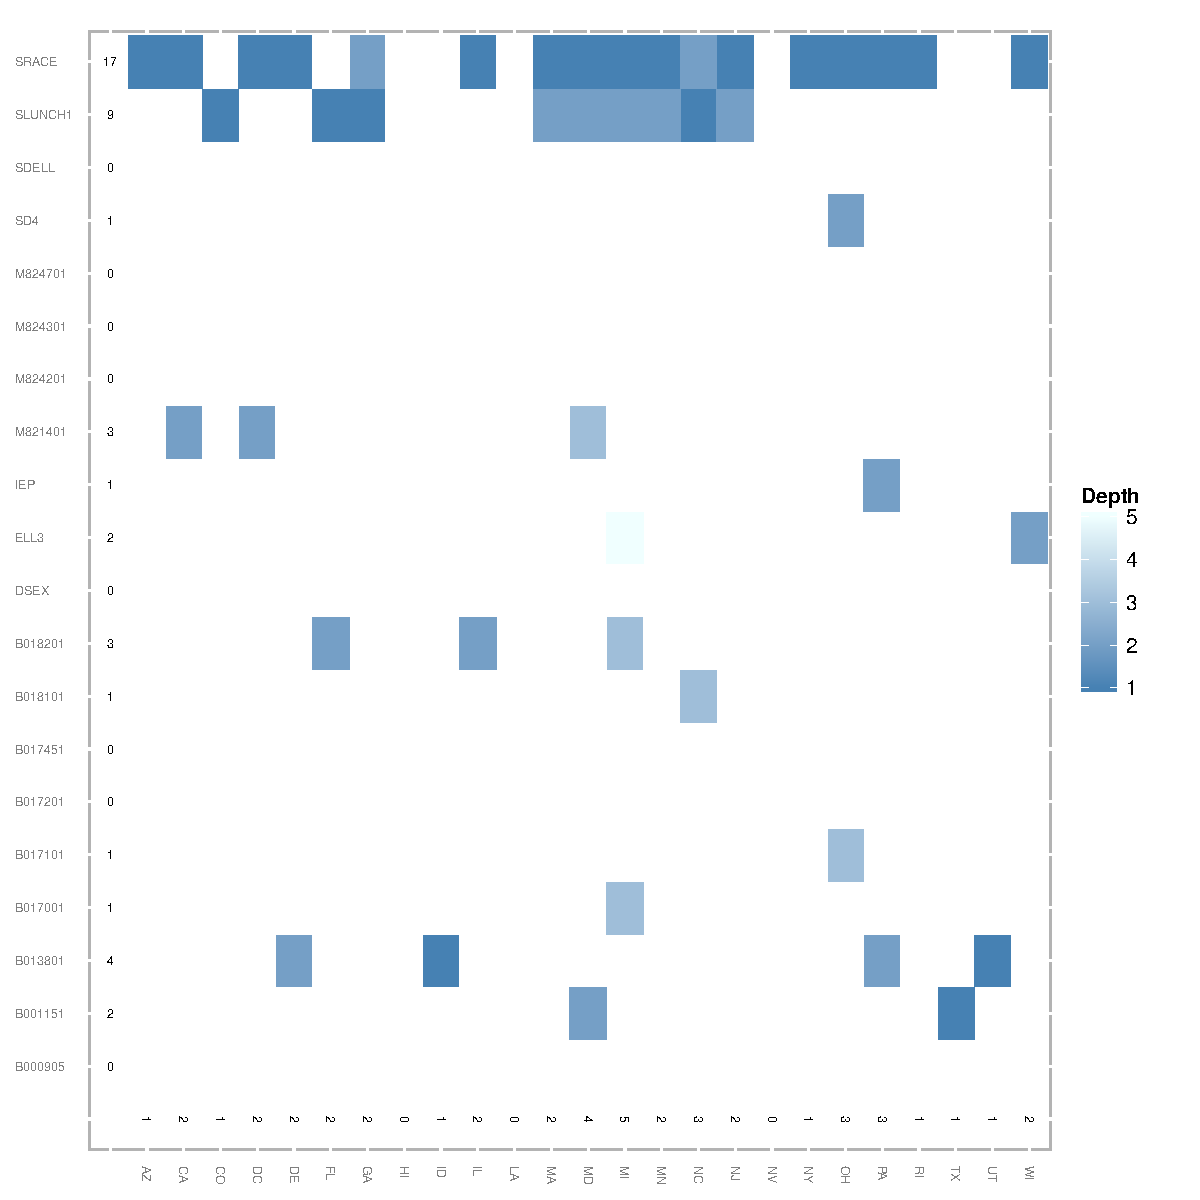
\includegraphics[width=\textwidth]{../Figures2009/g4math-mlpsa-ctree-heat.pdf}
\caption{Heat Map of Relative Importance of Covariates for Phase I: Grade 4 Math}
\label{fig:g4math-mlpsa-ctree-heat}
\end{center}
\end{figure}

\begin{figure}[h]
\begin{center}
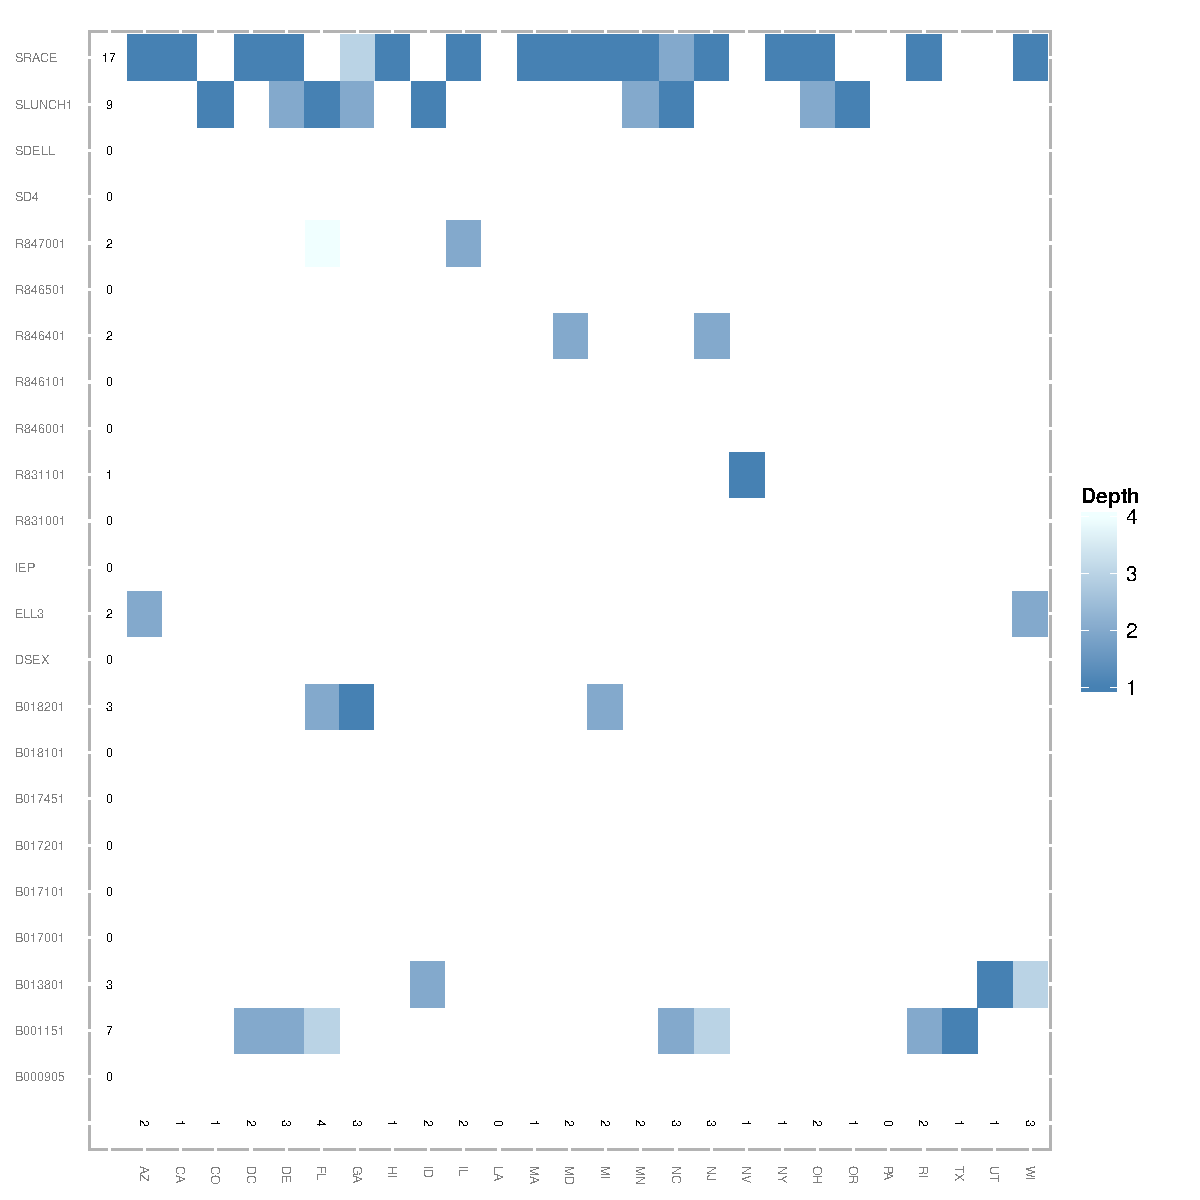
\includegraphics[width=\textwidth]{../Figures2009/g4read-mlpsa-ctree-heat.pdf}
\caption{Heat Map of Relative Importance of Covariates for Phase I: Grade 4 Reading}
\label{fig:g4read-mlpsa-ctree-heat}
\end{center}
\end{figure}

\begin{figure}[h]
\begin{center}
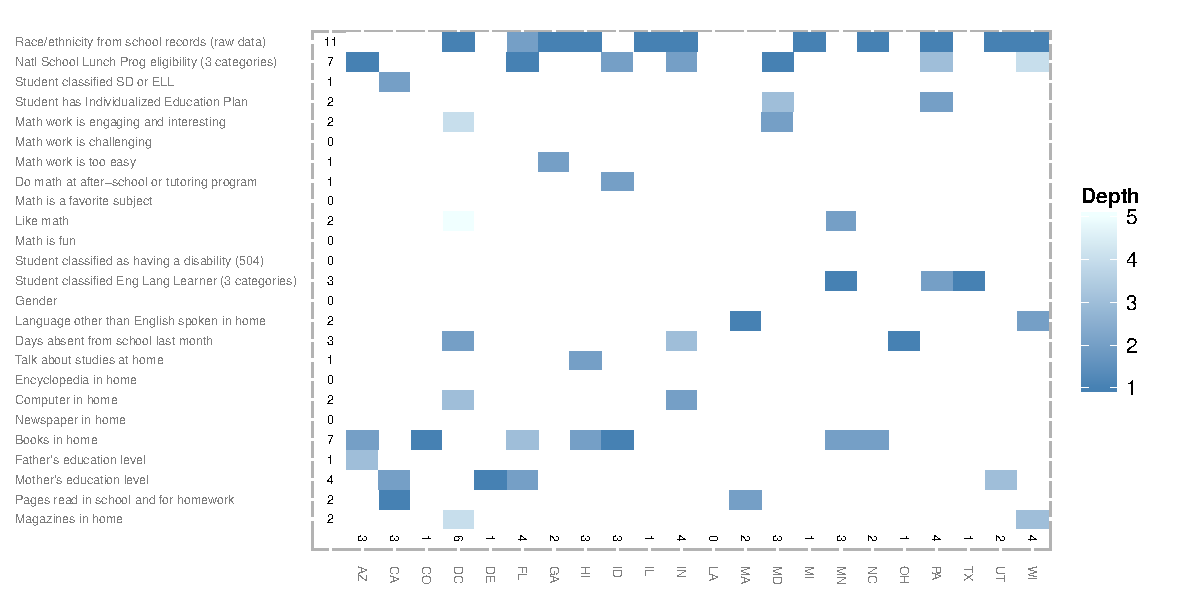
\includegraphics[width=\textwidth]{../Figures2009/g8math-mlpsa-ctree-heat.pdf}
\caption{Heat Map of Relative Importance of Covariates for Phase I: Grade 8 Math}
\label{fig:g8math-mlpsa-ctree-heat}
\end{center}
\end{figure}

\begin{figure}[h]
\begin{center}
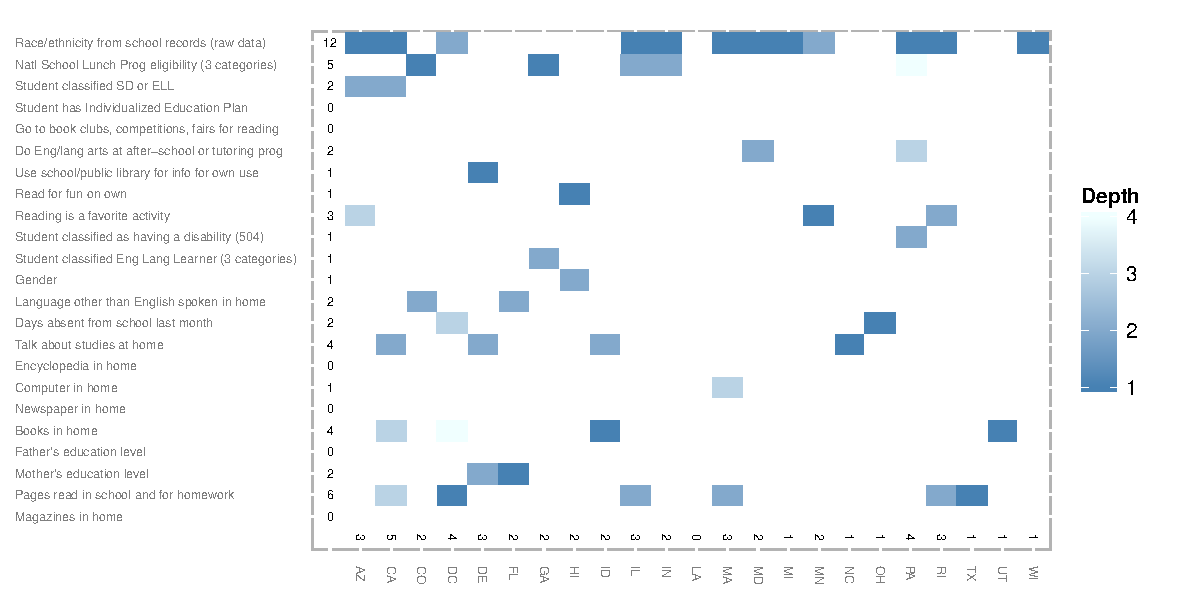
\includegraphics[width=\textwidth]{../Figures2009/g8read-mlpsa-ctree-heat.pdf}
\caption{Heat Map of Relative Importance of Covariates for Phase I: Grade 8 Reading}
\label{fig:g8read-mlpsa-ctree-heat}
\end{center}
\end{figure}


%==================== Appendix J ====================================================================
\clearpage
\addcontentsline{toc}{subsection}{Appendix J: Distribution of NAEP Scores for Matched vs. Unmatched Public School Students}
\subsection*{Appendix J\\Distribution of NAEP Scores for Matched vs. Unmatched Public School Students}
\label{appendixPublicDensity}

The figures in this appendix represent the distributions of matched and unmatched public school students as identified by the full logistic regression model. These models were chosen since they resulted in the largest number of unmatched public school students vis-\`a-vis stratification. It should be noted that for some states there may be only one density line. This indicates that all public school students within that state were either all matched or all not matched.

%\begin{figure}[h]
%\begin{center}
%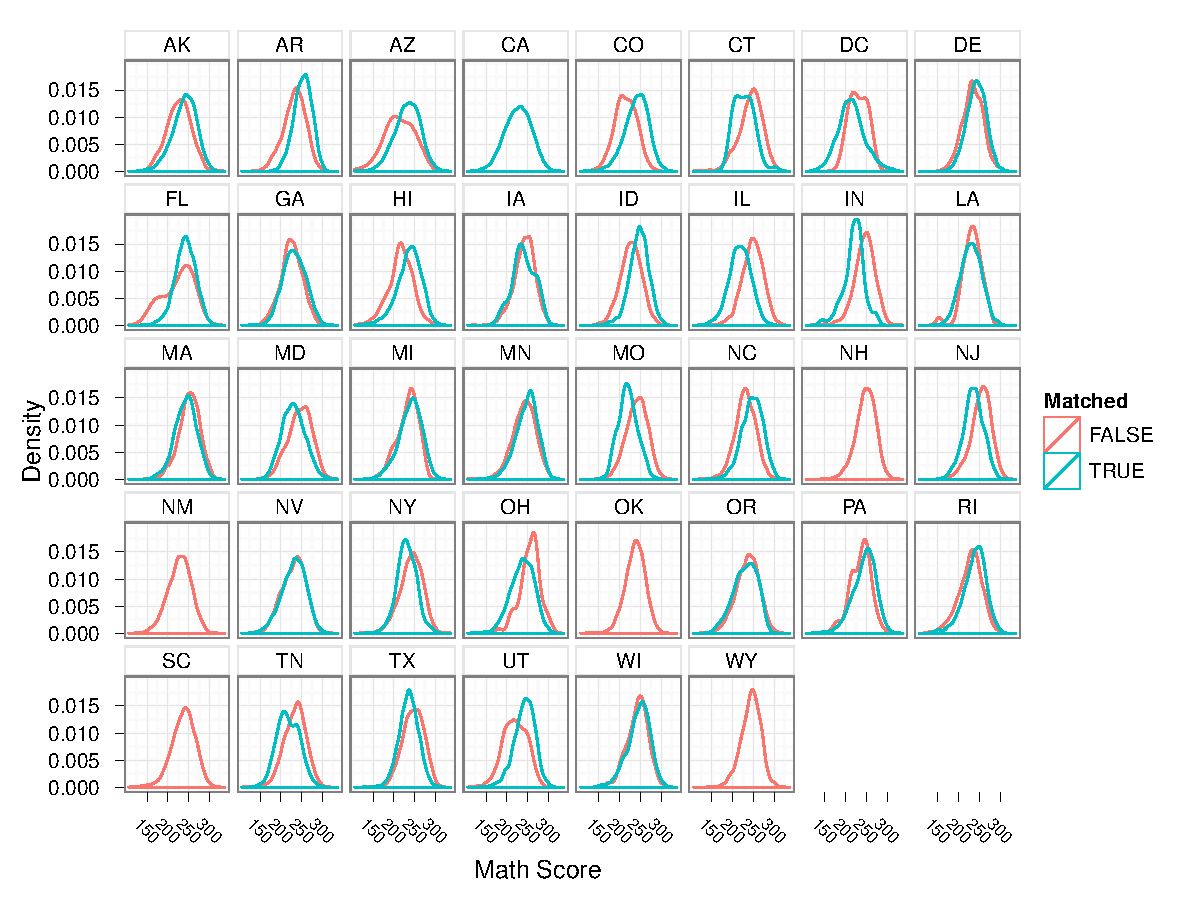
\includegraphics[height=\textwidth,angle=90]{../Figures/g4mathlrPublicDensity.pdf}
%\caption{Density Distribution of Grade 4 Math: Matched vs. Unmatched Public School Students}
%\label{fig:g4reading:publicdensity}
%\end{center}
%\end{figure}
%\clearpage
%
%\begin{figure}[h]
%\begin{center}
%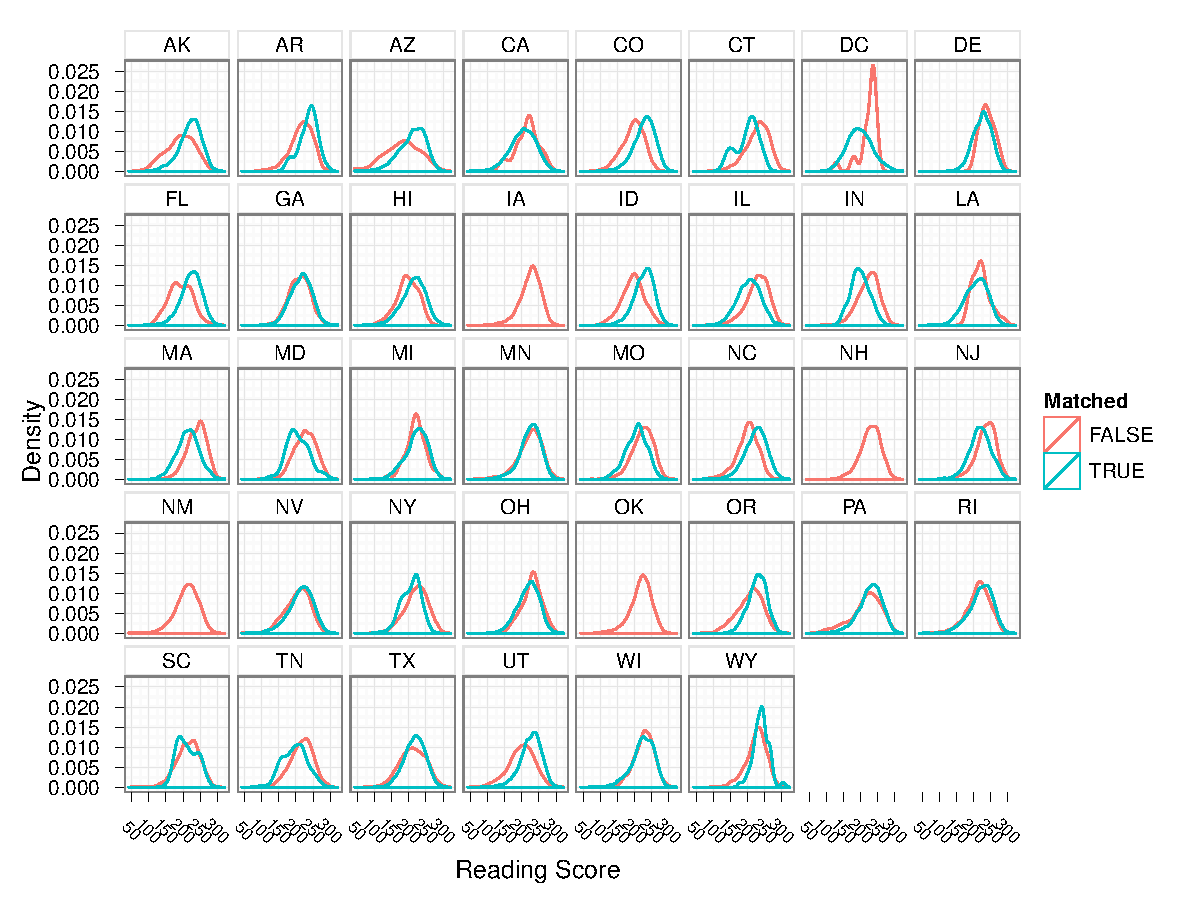
\includegraphics[height=\textwidth,angle=90]{../Figures/g4readinglrPublicDensity.pdf}
%\caption{Density Distribution of Grade 4 Reading: Matched vs. Unmatched Public School Students}
%\label{fig:g4reading:publicdensity}
%\end{center}
%\end{figure}
%\clearpage
%
%\begin{figure}[h]
%\begin{center}
%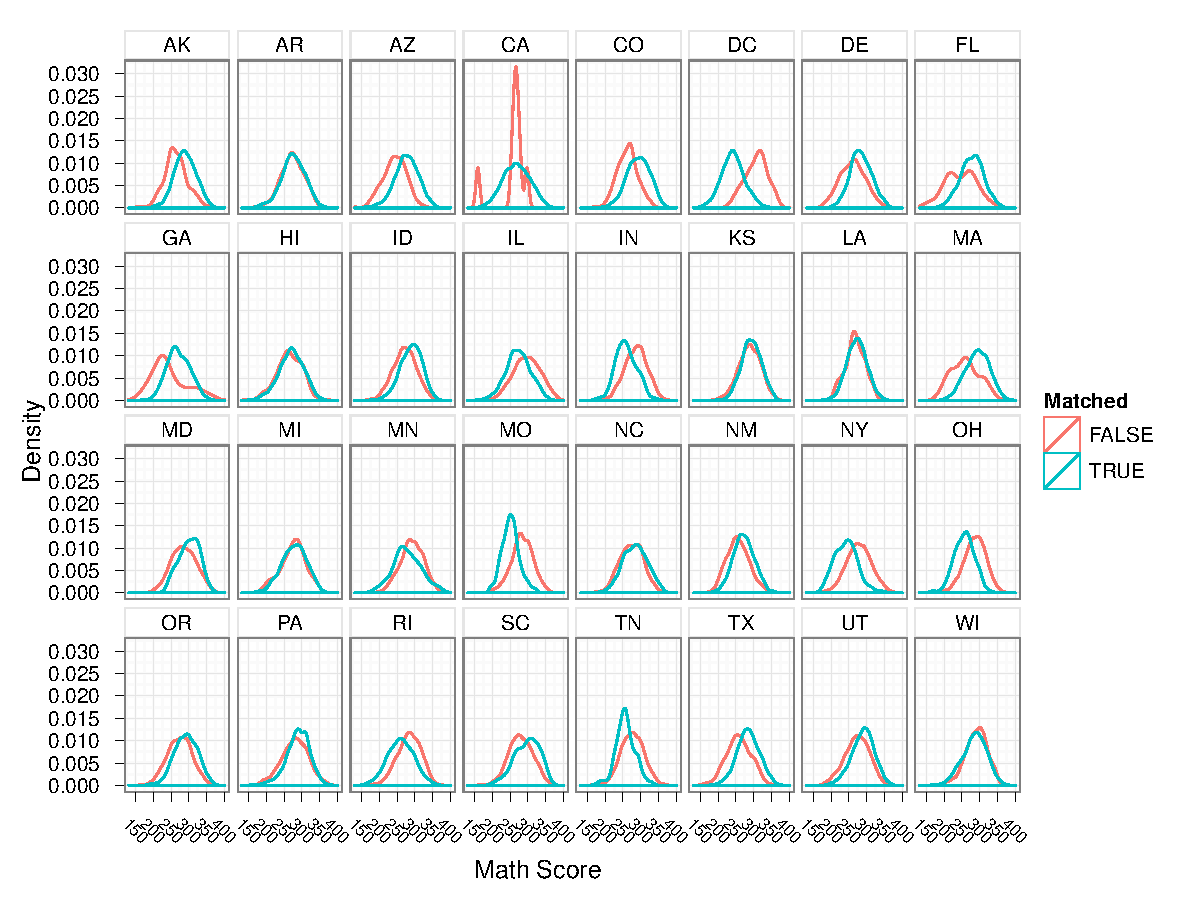
\includegraphics[height=\textwidth,angle=90]{../Figures/g8mathlrPublicDensity.pdf}
%\caption{Density Distribution of Grade 8 Math: Matched vs. Unmatched Public School Students}
%\label{fig:g8reading:publicdensity}
%\end{center}
%\end{figure}
%\clearpage
%
%\begin{figure}[h]
%\begin{center}
%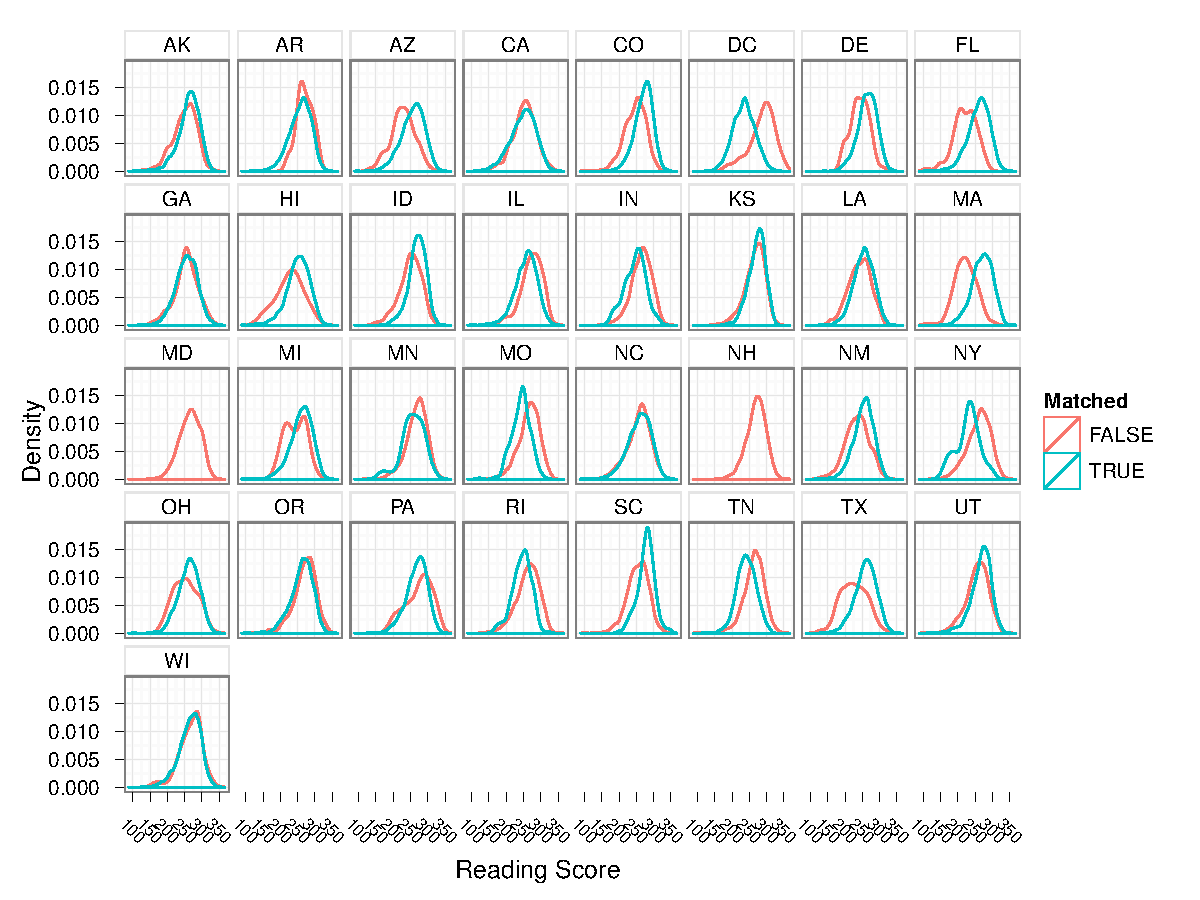
\includegraphics[height=\textwidth,angle=90]{../Figures/g8readinglrPublicDensity.pdf}
%\caption{Density Distribution of Grade 8 Reading: Matched vs. Unmatched Public School Students}
%\label{fig:g8reading:publicdensity}
%\end{center}
%\end{figure}
%\clearpage

%==================== Appendix J ====================================================================
\clearpage
\addcontentsline{toc}{subsection}{Appendix K: multilevelPSA R Package}
\subsection*{Appendix K\\multilevelPSA R Package}
\label{multilevelPSAPackage}

The \texttt{multilevelPSA} R package was developed, in part, to conduct the analysis for this dissertation. It is available from the Comprehensive R Archive Network (CRAN) at \url{http://cran.r-project.org/web/packages/multilevelPSA}. The latest version can be installed using the \texttt{install.packages} function in R:

\begin{verbatim}
> install.packages('multilevelPSA', repos='http://cran.r-project.org')
\end{verbatim}

The following list provides brief descriptions of the key functions in the \texttt{multilevelPSA} package. More information is available vis-\`a-vis the R help system.

\renewcommand{\descriptionlabel}[1]{\hspace{\labelsep}\textbf{\texttt{#1}}}
\begin{description}
\item[getPropensityScores] Returns a data frame with two columns corresponding to the level 2 variable and the fitted value from the logistic regression.
\item[getStrata] Returns a data frame with two columns corresponding to the level 2 variable and the leaves from the conditional inference trees.
\item[loess.plot] Loess plot with density distributions for propensity scores and outcomes on top and right, respectively.
\item[missing.plot] Returns a heat map graphic representing missingness of variables grouped by the given grouping vector.
\item[mlpsa] This function will perform phase II of the multilevel propensity score analysis.
\item[plot.mlpsa] Creates the multilevel assessment plot.
\item[mlpsa.circ.plot] Plots the results of a multilevel propensity score model.
\item[mlpsa.ctree] Estimates propensity scores using the recursive partitioning in a conditional inference framework.
\item[mlpsa.difference.plot] Creates a graphic summarizing the differences between treatment and comparison groups within and across level two clusters.
\item[mlpsa.distribution.plot] Plots distribution for either the treatment or comparison group.
\item[mlpsa.logistic] Estimates propensity scores using logistic regression.
\item[psrange] Estimates models with increasing number of comparison subjects starting from 1:1 to using all available comparison group subjects.
\item[plot.psrange] Plots the results of \texttt{psrange}.
\item[tree.plot] Heat map representing variables used in a conditional inference tree across level 2 variables.
\end{description}




\end{document}
